\documentclass[12pt]{article}
\usepackage[a4paper, margin=20mm, marginparwidth = 1.8cm]{geometry}
\usepackage{graphicx}
\usepackage{float}
\usepackage{fontspec}
\usepackage{booktabs}
\usepackage{url}
\usepackage{appendix}
\usepackage{subfigure}
\usepackage{bm}
\usepackage{amsfonts}
\usepackage{amsmath}
\usepackage{multirow}

\usepackage[hidelinks]{hyperref}
\usepackage{ocgx2}

\newcounter{step}[subsubsection]
\renewcommand{\thestep}{\arabic{step}}
\newcommand{\step}{\refstepcounter{step}\textbf{Step \thestep:} }


\linespread{1.15}

\setmainfont{Times New Roman}
\pagenumbering{roman}

\begin{document}
\input{title}

\input{contents}
\pagebreak

\section{Week 1 - Introduction}
\pagenumbering{arabic}
\subsection{Assessments}

\noindent\textbf{Early Semester Feedback Task}

\begin{itemize}
    \item Multiple choice, True/False
    \item On Canvas – Open book
    \item Syllabus – Week 1 to 3
    \item Held in Week 4
\end{itemize}

\bigskip

\noindent\textbf{Viva}

\begin{itemize}
    \item Oral quiz held in tutorials
    \item Secured assessment – No notes allowed
    \item Syllabus – Week 1 to Week 7
    \item Held in Week 8
\end{itemize}

\bigskip

\noindent\textbf{Group Assignment}

\begin{itemize}
    \item Groups of 4-5 people
    \item "Topic of assessment"
    \item Submission in Week 12
\end{itemize}

\bigskip

\noindent\textbf{Final Exam}

\begin{itemize}
    \item Restrictive open book – 1 page both side
    \item Case Study based Questions
    \item Held in Exam week
\end{itemize}

\subsection{Basic Concept}

\subsubsection{Knowledge, Skills and Expertise}

\noindent\textbf{Knowledge}: Knowing about something, how to do it.

\noindent\textbf{Skills}: Being able to do it – competence, capability

\noindent\textbf{Expertise = Knowledge + Skills}

\subsubsection{Profession}

\noindent\textbf{Profession}: An occupation requiring specialized education, expertise, and practical skills. It is guided by ethical standards, often regulated by professional bodies, and serves the public by addressing complex societal needs.

\subsubsection{Practice}

\noindent\textbf{Practice}: refers to the repeated application of knowledge, skills, or activities to improve performance or maintain proficiency. It can also mean the actual work done within a profession or discipline.

\subsubsection{Professionalism}

\noindent\textbf{Professionalism}: is the conduct, behavior, and attitude expected of someone in a professional role. It reflects a commitment to competence, ethics, integrity, and respect in the workplace.

\bigskip

\noindent\textbf{Key aspects}:

\begin{itemize}
    \item Competence - having the necessary knowledge and skills.
    \item Accountability - taking responsibility for your actions.
    \item Ethical Behavior - acting with honesty, fairness, and integrity.
    \item Reliability - being dependable and consistent.
    \item Respect and courtesy - treating others with dignity and professionalism
\end{itemize}

\subsubsection{Being an IT professional}

\noindent \textbf{Being an IT professional} goes beyond just working with technology. It is about expertise, responsibility, and ethics in using technology to solve problems and create value.

\noindent\textbf{Core skills in today's world}: Tech Skills = Capability. Soft Skills = Adaptability. Tech Can Be Taught, Soft Skills Take Time.

\subsection{IT Careers}

\indent 

In the fast-evolving world of Information Technology, career paths can vary greatly depending on your experience, skills, and specialization. Whether you're a student just entering the field or a seasoned professional, job roles and responsibilities grow with you.

The next few slides will showcase real-world examples of IT job descriptions across different stages of an IT career, from entry-level roles for recent graduates to mid-level positions, and then senior or specialized roles.

This will help you understand how expectations change over time and what you can work toward as you grow in the industry

\subsubsection{Progression of IT careers}

\noindent\textbf{Year 0-2}: Entry level / Graduate roles

\begin{itemize}
    \item \textbf{Job Titles}: IT Support, Junior Developer, Data Analyst, QA Tester, Business Analyst
    \item \textbf{Focus}: Building foundational technical skills, learning industry tools, working under supervision
    \item \textbf{Skills Gained}: Coding, troubleshooting, system usage, documentation, teamwork
\end{itemize}

\bigskip

\noindent\textbf{Year 3-5}: Intermediate / Associate roles

\begin{itemize}
    \item \textbf{Job Titles}: Software Engineer, Systems Analyst, DevOps Engineer, Data Engineer, Cybersecurity Analyst
    \item \textbf{Focus}: Managing projects/components independently, starting to mentor juniors, deeper domain knowledge
    \item \textbf{Skills Gained}: Full-stack development, cloud computing, process automation, security practices
\end{itemize}

\bigskip

\noindent\textbf{Year 6-8}:

\begin{itemize}
    \item \textbf{Job Titles}: Senior Developer, Solutions Architect, Tech Lead, Product Manager, Senior Analyst
    \item \textbf{Focus}: Leading projects or teams, shaping systems or product direction, engaging stakeholders
    \item \textbf{Skills Gained}: Leadership, system design, cross-functional collaboration, technical decision-making
\end{itemize}

\bigskip

\noindent\textbf{Year 9-12+}:

\begin{itemize}
    \item \textbf{Job Titles}: IT Manager, Engineering Manager, Enterprise Architect, CTO, CIO
    \item \textbf{Focus}: Organizational strategy, team management, innovation, aligning IT with business goals
    \item \textbf{Skills Gained}: Strategic planning, budgeting, stakeholder management, organizational leadership
\end{itemize}

\bigskip

\noindent\textbf{Alternate Paths}:

\begin{itemize}
    \item Consulting - Moving into IT consulting or advisory roles
    \item Research - Pursuing a PhD or research-intensive career in AI, HCI, etc.
    \item Entrepreneurship - Founding or joining a startup
    \item Specialization - Becoming an expert in niche areas (e.g., cybersecurity, ML/AI, blockchain)
\end{itemize}

\subsubsection{Typical activities in IT careers}

\begin{table}[h]
\centering
\begin{tabular}{|c|c|c|c|cl|}
\hline
\textbf{Technical}     & \textbf{\begin{tabular}[c]{@{}c@{}}Analytical\&\\ Problem solving\end{tabular}} & \textbf{\begin{tabular}[c]{@{}c@{}}Project\&Process\\ Management\end{tabular}} & \textbf{\begin{tabular}[c]{@{}c@{}}Collaboration \&\\ Communication\end{tabular}} & \multicolumn{2}{c|}{\textbf{\begin{tabular}[c]{@{}c@{}}Learning \&\\ Innovation\end{tabular}}} \\ \hline
\textbf{Coding}        & Troubleshooting                                                                 & Project planning                                                               & Stakeholder comm                                                                  & \multicolumn{2}{c|}{Continuous learn}                                                          \\ \hline
\textbf{Testing}       & System design                                                                   & Agile/Scrum                                                                    & Team collaboration                                                                & \multicolumn{2}{c|}{Evaluating tools}                                                          \\ \hline
\textbf{Debugging}     & Data collection                                                                 & Time management                                                                & User training                                                                     & \multicolumn{2}{c|}{Adopting innovation}                                                       \\ \hline
\textbf{Prototyping}   & Data analysis                                                                   & Cost management                                                                & Managing vendors                                                                  & \multicolumn{2}{c|}{Knowledge share}                                                           \\ \hline
\textbf{Cybersecurity} & Reporting                                                                       & Quality assurance                                                              & Client interactions                                                               & \multicolumn{2}{c|}{Innovating}                                                                \\ \hline
\end{tabular}
\end{table}

\subsection{IT in Organizations}

\subsubsection{Role of IT}

\indent

The \textbf{role of IT} (Information Technology) is to enable, support, and transform the way individuals, businesses, and governments \textbf{store, process, communicate, and access information}.

It serves as the backbone of modern operations and innovation.

\bigskip

\noindent\textbf{Core roles of IT}:

\begin{itemize}
    \item Enabling Communication and collaboration
    \item Data management and storage
    \item Process automation
    \item System development and maintenance
    \item Cybersecurity and risk management
    \item Supporting innovation and digital transformation
    \item Technical support and troubleshooting
\end{itemize}

\subsubsection{Role of IT in organizations}

\indent

IT provides value to an organization through changing the way in which business functions and processes are carried out.

IT provides value by providing new functions and enabling new business models.

\subsection{Changing Business Landscape}

\noindent The 4 key forces that reshape how organizations operate and compete:

\begin{itemize}
    \item Business drivers
    \item Technology drivers
    \item Customer expectations
    \item Market trends
\end{itemize}

\subsection{Question}

\subsubsection{End of lecture questions}

\begin{itemize}
    \item Define the following terms and explain how they differ: Profession, Practice, Professionalism
    \item What is the purpose of INFO5990, and how does it prepare students for IT careers?
    \item List three ways technological advancement has changed the nature of IT careers.
    \item Briefly explain the role of IT in modern organizations. Give two examples.
    \item Describe three soft skills that are essential in IT careers and explain why they are important.
\end{itemize}

\subsubsection{Case-study based Questions}

\indent

Alex is a recent IT graduate who just started a job as a junior systems analyst at a large consulting firm. In their first few weeks, they realized that although they had strong technical skills, they struggled with stakeholder communication and time management. Their team lead recommended that they revisit the concepts taught in INFO5990 to improve their workplace professionalism and soft skills.

\bigskip

\noindent\textbf{Question}:

\begin{itemize}
    \item Identify two aspects of professionalism that Alex is currently struggling with. Justify your answer.
    \item How could Alex’s understanding of “professional practice” help him improve his performance and confidence at work?
    \item Suggest three strategies Alex can implement to enhance his soft skills, drawing from INFO5990 learning.
    \item Explain how changing business landscapes demand new skillsets in IT roles, and how Alex can prepare for that.
\end{itemize}
\pagebreak

\section{Week 2 - Creating organisational value from IT investments}
\subsection{Organisation}

\textbf{Organisation}: A structured group of people working together to achieve specific goals or purposes.

\begin{itemize}
    \item \textbf{Formal}: A company, school, government agency, or non-profit.
    \item \textbf{Informal}: A community group or club.
\end{itemize}

\subsubsection{Characteristics}

\begin{itemize}
    \item \textbf{Purpose}: A mission or objective that guides its activities.
    \item \textbf{People}: Individuals with different roles, responsibilities, and skills.
    \item \textbf{Structure}: A defined hierarchy that outlines how tasks are divided and coordinated.
    \item \textbf{System} Methods for communication, decision making, and operations.
    \item \textbf{Resources} They utilize human, financial, technological, and physical resources.
\end{itemize}

\subsubsection{Organisation VS Business}

\indent

\textbf{Organisation}: a \textbf{broad term} that refers to any group of people working together in a structured way to achieve a common goal. \textbf{Not always profit-driven.}

\textbf{Business}: \textbf{a type of Organisation} whose \textbf{primary goal is to make a profit} by providing goods or services.

\begin{table}[h]
    \centering
    \begin{tabular}{c|c}
        \hline
        Organisation & Business \\\hline
        Non-profits – Red Cross & Startups – Canva\\
        Governments – NSW Health & Corporations – Apple\\
        Universities – University of Sydney & Small Businesses – Local cafes\\
        Clubs – Local sports club & \\\hline
    \end{tabular}
    \caption{Some examples}
\end{table}

\subsection{Organisational Structure}

\textbf{Organisational Structure}: 

It defines \textbf{how tasks, responsibilities, and authority are distributed} within an Organisation. 

It shows the \textbf{hierarchy, reporting lines}, and how different roles and departments \textbf{interact and coordinate} with each other.

\subsubsection{Why Organisational Structure Important?}

\begin{itemize}
    \item Clarifies who reports to whom
    \item Defines decision-making authority
    \item Improves efficiency and communication
    \item Helps manage growth and change
\end{itemize}

\subsubsection{Type of Organisational Structure}

\begin{itemize}
    \item \textbf{Functional}: Groups employees based on specialized roles or functions.
    \item \textbf{Matrix}: Employees report to two managers - one for function, one for project.
    \item \textbf{Flat}: Few or no levels of middle management. Common in startups or small Organisations.
    \item \textbf{Hierarchical}: Traditional structure with clear top-down command and multiple layers of authority.
\end{itemize}

\subsubsection{Organisational Structures - Functional}

\begin{figure}[h]
    \centering
    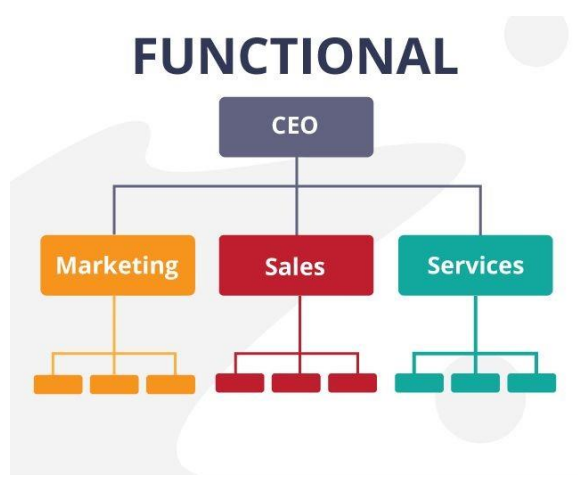
\includegraphics[width=0.5\linewidth]{figures/Week 2/Functional.png}
\end{figure}

\noindent\textbf{Functional}: Organisation is divided into departments 
based on specific functions (e.g., IT, HR, Finance, Marketing).

\noindent\textbf{Best For:} Large or growing organisations with clearly defined departments (e.g., tech companies, banks, \textbf{Microsoft}).

\bigskip

\noindent\textbf{Pros:}

\begin{itemize}
    \item Specialisation leads to efficiency
    \item Clear roles and responsibilities
    \item Easier to manage and scale by department
\end{itemize}

\bigskip

\noindent\textbf{Cons:}

\begin{itemize}
    \item Limited communication across departments
    \item Can create silos and reduce flexibility
\end{itemize}

\subsubsection{Organisational Structures - Matrix}

\begin{figure}[h]
    \centering
    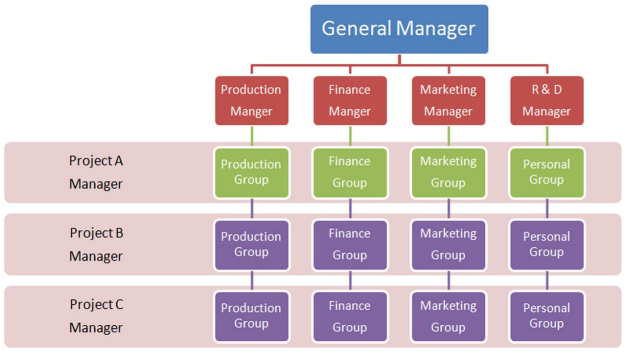
\includegraphics[width=0.8\linewidth]{figures/Week 2/Matrix.png}
\end{figure}

\noindent\textbf{Matrix}: Employees report to more than one manager, typically by function and project/team.

\noindent\textbf{Best For:} Project-based or global companies (e.g., consulting firms, R\&D, IT services companies, \textbf{Google}).

\bigskip

\noindent\textbf{Pros:}

\begin{itemize}
    \item Efficient use of resources across projects
    \item Encourages teamwork and cross functional skills
    \item Increases flexibility and adaptability
\end{itemize}

\bigskip

\noindent\textbf{Cons:}

\begin{itemize}
    \item Dual authority can cause confusion
    \item Requires strong communication and coordination
\end{itemize}

\subsubsection{Organisational Structures - Flat}

\begin{figure}[h]
    \centering
    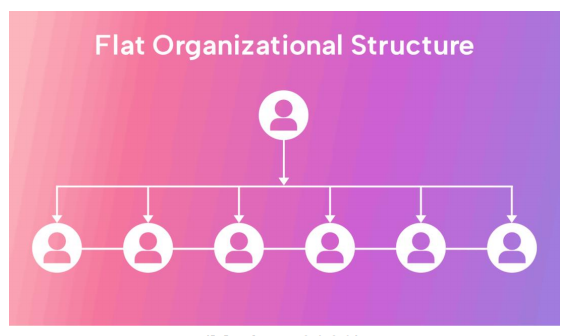
\includegraphics[width=0.5\linewidth]{figures/Week 2/Flat.png}
\end{figure}

\noindent\textbf{Flat}: Few or no levels of middle management between staff and leadership. Everyone is closer to decision-making.

\noindent\textbf{Best For:} Startups or small teams where agility and speed matter more than hierarchy. (e.g., \textbf{Valve})

\bigskip

\noindent\textbf{Pros:}

\begin{itemize}
    \item Fast communication and decision making
    \item Encourages innovation and collaboration
    \item Flexible and adaptive
\end{itemize}

\bigskip

\noindent\textbf{Cons:}

\begin{itemize}
    \item Can lead to confusion in roles/responsibilities
    \item Not scalable for large teams
\end{itemize}

\subsubsection{Organisational Structures - Hierarchical}

\begin{figure}[h]
    \centering
    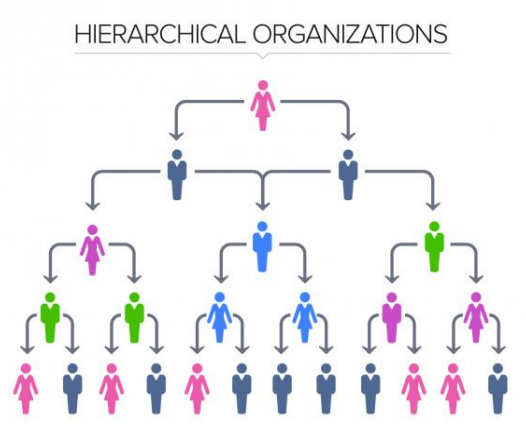
\includegraphics[width=0.5\linewidth]{figures/Week 2/Hierarchical.png}
\end{figure}

\noindent\textbf{Hierarchical}: Traditional top-down approach with multiple levels of authority and a clear chain of command.

\noindent\textbf{Best For:} Government bodies, large enterprises, 
and traditional corporations. (e.g., \textbf{IBM})

\bigskip

\noindent\textbf{Pros:}

\begin{itemize}
    \item Clear reporting lines and accountability
    \item Stable and easy to manage large teams
    \item Supports growth and delegation
\end{itemize}

\bigskip

\noindent\textbf{Cons:}

\begin{itemize}
    \item Slower decision-making
    \item Can stifle creativity and employee autonomy
\end{itemize}

\subsection{Value and Organisational Value}

\subsubsection{Value}

\textbf{Value}: refers to the \textbf{worth}, \textbf{usefulness}, or \textbf{benefit} of something.

\begin{itemize}
    \item Tangible (e.g., Money, Products)
    \item Intangible (e.g., Trust, Satisfaction)
\end{itemize}

\subsubsection{Organisational Value}

\textbf{Organisational Value}: refers to the \textbf{value created}, \textbf{delivered}, and \textbf{sustained} by an Organisation for its stakeholders, including customers, employees, shareholders, and society.

\subsubsection{Value VS Organisational Value}

% Please add the following required packages to your document preamble:
% \usepackage{multirow}
\begin{table}[h]
\begin{tabular}{|c|c|l|}
\hline
\multirow{2}{*}{Scope}        & Value                & \begin{tabular}[c]{@{}l@{}}Broad and general – can apply to anything, anyone, or any idea,\\ not limited to a business context.\end{tabular}                                    \\ \cline{2-3} 
                              & Organisational Value & \begin{tabular}[c]{@{}l@{}}Narrower and specific - relates only to what an organisation \\ creates, delivers, and sustains through its operations and mission.\end{tabular}     \\ \hline
\multirow{2}{*}{Focus}        & Value                & \begin{tabular}[c]{@{}l@{}}Centers on the worth of an individual item, idea, or experience \\ (e.g., the usefulness of a product).\end{tabular}                                 \\ \cline{2-3} 
                              & Organisational Value & \begin{tabular}[c]{@{}l@{}}Centers on the overall value an organisation, provides through \\ its products, services, operations, and impact.\end{tabular}                       \\ \hline
\multirow{2}{*}{Stakeholders} & Value                & \begin{tabular}[c]{@{}l@{}}Typically individual or small-scale - the person using or \\ valuing the object (e.g., a buyer).\end{tabular}                                        \\ \cline{2-3} 
                              & Organisational Value & \begin{tabular}[c]{@{}l@{}}Includes multiple stakeholders - such as customers, employees, \\ shareholders, suppliers, and the community.\end{tabular}                           \\ \hline
\multirow{2}{*}{Measurement}  & Value                & \begin{tabular}[c]{@{}l@{}}Often subjective - based on personal perception, \\ emotional attachment, or market resale value.\end{tabular}                                       \\ \cline{2-3} 
                              & Organisational Value & \begin{tabular}[c]{@{}l@{}}Quantified through metrics like KPIs, profit margins, customer \\ satisfaction, brand reputation, innovation, and social impact.\end{tabular}        \\ \hline
\multirow{2}{*}{Example}      & Value                & A car has value because it provides transport, could be sold, etc.                                                                                                              \\ \cline{2-3} 
                              & Organisational Value & \begin{tabular}[c]{@{}l@{}}Toyota creates Organisational value by offering reliable cars to \\ the customers, jobs to its employees, returns to shareholders, etc.\end{tabular} \\ \hline
\end{tabular}
\end{table}



\subsection{IT investment}

\noindent\textbf{IT investment}: refers to the allocation of financial, human, and technological resources into information technology systems, tools, or services to support or improve an Organisation’s operations, performance, or strategic goals.

These resources and capabilities can be internally owned by the Organisation (insourced) or externally sourced (outsourced)

\subsubsection{Resources VS Capabilities}

\noindent

\textbf{Resources}: refer to what an Organisation owns.

\begin{itemize}
    \item Tangible (e.g., property, machinery, hardware)
    \item Intangible (e.g., knowledge, skills of employees, policies)
\end{itemize}

\textbf{Capabilities}: refer to what an Organisation can do by using those resources.

\noindent A capability is the ability to execute a specified course of action to achieve certain outcomes based on the resources available such as skills and technology.

\subsubsection{How do these concepts link together?}

\begin{table}[h]
\centering
\begin{tabular}{|c|l|}
\hline
\multirow{2}{*}{Organisation}  & Structure, people, and processes that drive operations.             \\ \cline{2-2} 
                               & Provides the foundation for strategy and delivery.                  \\ \hline
\multirow{2}{*}{IT Investment} & Technology enables efficiency, innovation, and scale.               \\ \cline{2-2} 
                               & Examples: Automation, data analytics, cloud, AI.                    \\ \hline
\multirow{3}{*}{Value}         & The result of organisational effort and tech enablement.            \\ \cline{2-2} 
                               & Benefits for stakeholders: customers, employees, investors, society \\ \cline{2-2} 
                               & Examples: Profits, Dividends, Operational efficiency, etc.          \\ \hline
\end{tabular}
\end{table}

When business and IT are properly aligned and orchestrated, the result is 
Organisational value.

The benefits are measurable such as: Increased customer satisfaction, Operational efficiency, Revenue growth, Innovation, Competitive advantage.

\subsubsection{The critical role of IT in creating Organisational Value}

\indent

Information Technology (IT) plays a central role in helping Organisations create, deliver, and sustain value. 

In today’s digital world, IT is not just a support function - it’s a strategic enabler of innovation, efficiency, and competitiveness.

\bigskip

\noindent How?

\begin{itemize}
    \item \textbf{Improving operational efficiency}: Automation, cloud systems, databases
    \item \textbf{Enhances decision making}: Data analytics, BI tools, Artificial Intelligence
    \item \textbf{Drives innovation}: IoT, Blockchain, Agentic AI
    \item \textbf{Enables customer-centric strategies}: CRM systems, Self-service platforms
    \item \textbf{Supports scalability and flexibility}: AWS, GCP, Azure
\end{itemize}

\subsection{Aligning IT and Business}

\begin{figure}[h]
    \centering
    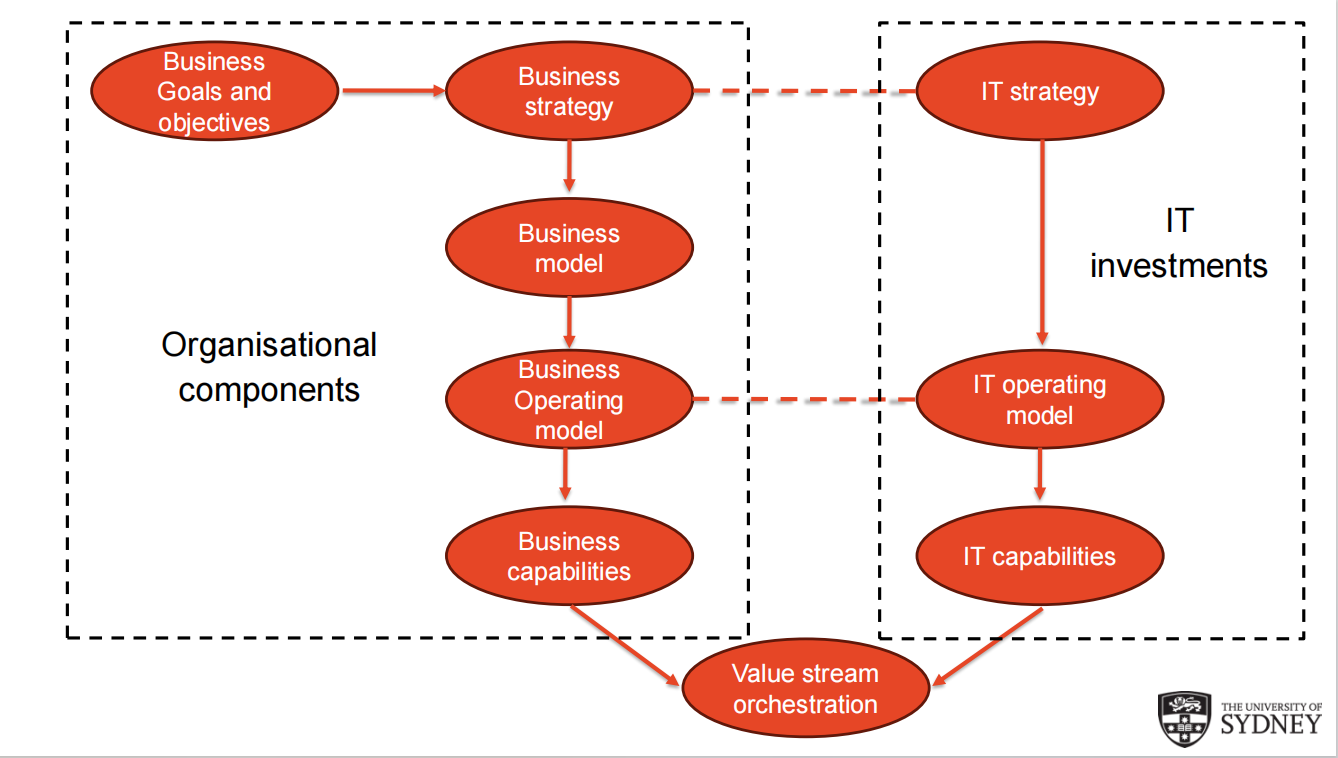
\includegraphics[width=0.8\linewidth]{figures/Week 2/two sides.png}
\end{figure}

\noindent Explanation:

\textbf{Organisation side}: This side outlines how an Organisation builds value through \textbf{business planning and operational structure}: Business goals and objectives, business strategy, business models, business operating models, and business capabilities.

\bigskip

\textbf{IT investment side}: This side shows how IT must align with business to support and enable value creation: IT strategy, IT operating model, and IT capabilities.

\subsubsection{Business goals and objectives}

\indent

Business goals and objectives are the foundation of all Organisational activity. They define the \textbf{vision}, \textbf{mission}, and \textbf{desired outcomes}. These guide both business and IT strategies. They \textbf{define value at the core}, because value begins with a clear understanding of what the Organisation
wants to achieve..

Objectives specify the methods, paths and metrics that can help an Organisation achieve a goal.

\subsubsection{Business goals VS Business objectives}

\indent

Business goals and business objectives are closely related, and the terms are sometimes used interchangeably. However, they are two different things.

\textbf{Business goals} represent the direction in which a company intends to go and 
define what the Organisation wants to achieve. 

\textbf{Business objective} specifies the methods and paths that can help a 
business achieve that goal.

\subsubsection{Business Strategy}

\indent

Business strategy outlines \textbf{how the Organisation will achieve its goals}. This includes choices around target markets, competitive positioning, resource allocations, etc. IT must be aligned with this strategy to be effective.

\textbf{Strategy drives both structure and technology direction.}

\subsubsection{IT strategy}

\indent

IT strategy is the roadmap for \textbf{how technology will support business strategy}. It focuses on digital transformation, infrastructure decisions, innovation plans, etc.

\textbf{IT strategy must be developed in lockstep with business strategy}.

\subsubsection{Business models}

\indent

The business model defines \textbf{how value is created, delivered, and captured}. It can be best show as a Business Model Canvas (BMC). Business models guide IT system requirements (e.g., eCommerce platforms, CRMs).

\textbf{A solid model ensures the strategy is executable.}

\subsubsection{Operating models}

\indent

An operating model is the blueprint for how value will be created and delivered to stakeholders.

It details how an Organisation configures and re-configures (orchestrates) its capabilities to create and deliver value to the Organisation to achieve its goals and strategic objectives.

An operating model also defines how the Organisation manages itself and its resources through its management processes, governance and culture.

Any change to the Organisation’s business models will require changes to the operating model.

\subsubsection{Business operating model}

\indent

The business operating model defines \textbf{how the organisation is structured and operates}. It describes centralization vs decentralization, business units and 
interdependencies, decision making authority, etc. Determines the IT support and governance model required.

\textbf{Operating model alignment enables efficient IT integration}.

\subsubsection{IT operating model}

\indent

Defines \textbf{how IT functions are structured and governed}. This includes IT service delivery, vendor management, project management, agile practices, etc. Must align with the business operating model.

\textbf{Efficient IT operations are critical for smooth execution}.

\subsubsection{Business capabilities}

\indent

Capabilities are the \textbf{skills, processes, and resources} the business uses to deliver value. Examples: logistics, R\&D, customer service, data analytics. Must be supported and often enhanced by IT (e.g., automation, AI, CRM systems).

\textbf{IT enables, enhances, or transforms these core capabilities.}

\subsubsection{IT capabilities}

\indent

IT capabilities refer to the technical strengths of the IT function. For example, system integration, cloud management, data analytics and reporting, cybersecurity, etc. These directly support and scale business capabilities.

\textbf{Strong IT capabilities are essential for digital competitiveness}.

\subsubsection{Value stream orchestration}

\indent

Value stream orchestration is about c\textbf{oordinating business and IT to deliver continuous value}. It involves synchronizing people, processes, and technology to \textbf{maximize the value delivered to stakeholders}. Enables smooth flow of value from idea to delivery.

\textbf{Orchestration ensures technology investments produce real 
business outcomes.}

\subsection{Best practices for IT investments}

\begin{itemize}
    \item Ensure every IT investment supports overall business goals.
    \item Engage business leaders in IT planning.
    \item Set measurable outcomes for each IT investment (e.g., cost savings, process efficiency, customer experience).
    \item Use KPIs to track ROI over time.
    \item Use a cost-benefit or value-risk matrix to rank IT initiatives.
    \item Focus on projects that provide both short-term wins and long-term value.
    \item Invest in technologies that can grow with the business (e.g., cloud, APIs, modular platforms).
    \item Avoid systems that lock the business into rigid structures.
    \item Encourage experimentation with emerging tech (AI, blockchain, IoT) in low risk areas.
    \item Balance innovation with practical business value
\end{itemize}

\subsection{Question}

\subsubsection{End of lecture questions}

\begin{itemize}
    \item Define the term “Organisation” and explain how it differs from a “business”.
    \item What is the difference between value and organisational value? Provide an example to illustrate.
    \item Explain the distinction between resources and capabilities with examples.
    \item List and briefly describe any three types of organisational structures.
    \item What is ‘value stream orchestration’ in the context of IT and business alignment?
\end{itemize}

\subsubsection{Case-study based questions}

\indent 

BrightCare is a mid-sized private healthcare organisation that specializes in telehealth services and digital patient records. The management has identified a need to increase organisational value by improving service delivery, enhancing patient satisfaction, and reducing operational costs. Currently, their systems are outdated, departments are siloed, and reporting is mostly manual.

The company has decided to:

\begin{itemize}
    \item Invest in a new cloud-based health information system (HIS)
    \item Hire a Chief Information Officer (CIO) to align IT strategy with the company’s vision
    \item Restructure from a functional model to a matrix structure to enable cross-departmental collaboration
\end{itemize}

The CIO proposes the following plan:

\begin{itemize}
    \item Define clear business goals (e.g., 30\% reduction in wait times, 95\% digital record accuracy)
    \item Align IT and business strategies by upgrading technology and retraining staff
    \item Build capabilities in data analytics and real-time reporting
    \item Implement value stream orchestration to connect IT workflows with patient care delivery
\end{itemize}

\noindent \textbf{Question}:

\begin{itemize}
    \item Identify two business goals BrightCare is trying to achieve through IT investment. How do these relate to Organisational value?
    \item What kind of Organisational structure was initially in place at BrightCare, and why is the move to a matrix structure beneficial in this context?
    \item Explain the role of the CIO in ensuring alignment between IT and business at BrightCare. What challenges might the CIO face?
    \item Evaluate whether the planned IT investment is likely to create organisational value. Justify your answer using concepts from the lecture.
\end{itemize}
\pagebreak

\section{Week 3 - IT Lifecycle and Project Management Essentials}
\subsection{Project Management Essentials}

\subsubsection{Project}

\noindent\textbf{Project}: A temporary endeavor undertaken to create a unique product, service, or result.

\noindent\textbf{Key characteristics}:

\begin{itemize}
    \item \textbf{Temporary}: Has a defined start and end date.
    \item \textbf{Unique}: Outcome is not routine, even if processes are repeatable.
    \item \textbf{Progressive elaboration}: Develops in steps and continues by increments.
\end{itemize}

\subsubsection{Success criteria}

\begin{itemize}
    \item \textbf{On-Time Delivery}: Meets the agreed schedule.
    \item \textbf{On-Budget}: Stays within allocated costs.
    \item \textbf{Meets Scope \& Quality}: Delivers all required features with acceptable quality standards.
    \item \textbf{Stakeholder Satisfaction}: End users, clients, and management are satisfied with the result.
    \item \textbf{Business Value}: Delivers measurable benefits such as cost savings, efficiency gains, or competitive advantage.
\end{itemize}

\subsubsection{Fail Reasons}

\begin{itemize}
    \item \textbf{Poor Scope Definition}: Unclear requirements, frequent changes.
    \item \textbf{Unrealistic Timelines or Budgets}: Overly optimistic estimates.
    \item \textbf{Weak Stakeholder Engagement}: Lack of buy-in from sponsors or end users.
    \item \textbf{Inadequate Risk Management}: Failing to anticipate and mitigate issues.
    \item \textbf{Poor Communication}: Misalignment between teams and stakeholders.
    \item \textbf{Resource Issues}: Lack of skilled staff or technology limitations.
\end{itemize}

\subsection{Project Management Methodologies}

\noindent\textbf{Project management methodology}: A structured approach that guides how a project is planned, executed, and delivered.

\noindent\textbf{Main purpose} of following a methodology:

\begin{itemize}
    \item Provides a framework to organise work
    \item Improves efficiency and communication
    \item Helps manage risks and deliver consistent results
\end{itemize}

\subsubsection{Waterfall Methodology}

\begin{figure}[h]
    \centering
    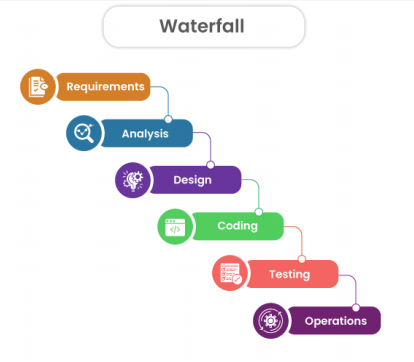
\includegraphics[width=0.5\linewidth]{figures/Week 3/Waterfall.png}
\end{figure}

Sequential, linear approach where each phase must be completed before the next begins.

\bigskip

\textbf{Benefits:}

\begin{itemize}
    \item Clear structure and documentation.
    \item Easy to manage with well-defined deliverables.
    \item Works well when requirements are stable.
\end{itemize}

When to use: Projects with fixed scope and minimal expected changes (e.g., compliance software, construction projects).

\bigskip

\textbf{Disadvantages:}

\begin{itemize}
    \item \textbf{Inflexibility to Changes}: Once a phase is completed, it’s difficult and costly to go back and make changes without affecting the entire project.
    \item \textbf{High Risk for Long Projects}: In lengthy projects, technology, user expectations, or market conditions might change before delivery, making the end product outdated.
    \item \textbf{Over-reliance on Initial Documentation}: The success of the project heavily depends on the accuracy and completeness of initial requirements and documentation.
    \item \textbf{Limited Stakeholder Engagement During Development} Once requirements are set, stakeholders are less involved until final delivery, which can lead to misalignment with expectations.
\end{itemize}

\subsubsection{Agile Methodology}

\begin{figure}[h]
    \centering
    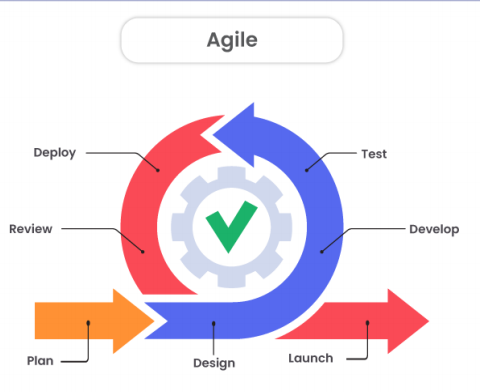
\includegraphics[width=0.5\linewidth]{figures/Week 3/Agile.png}
\end{figure}

Iterative, flexible approach focusing on delivering small, incremental improvements. Uses short work cycles called \textbf{sprints}.

\bigskip

\textbf{Benefits:}

\begin{itemize}
    \item Adapts to changing requirements.
    \item Encourages stakeholder feedback early and often.
    \item Delivers working software faster.
\end{itemize}

When to use: Projects where requirements are evolving (e.g., mobile apps, SaaS products)

\subsubsection{DevOps Approach}

\begin{figure}[h]
    \centering
    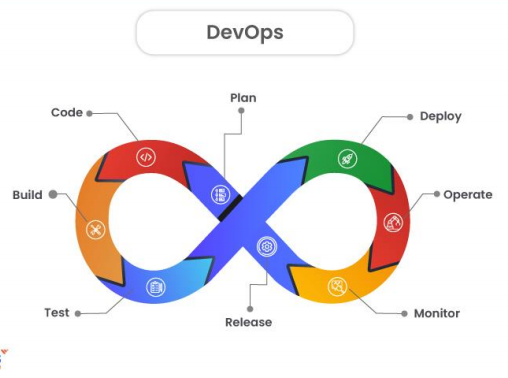
\includegraphics[width=0.5\linewidth]{figures/Week 3/DevOps.png}
\end{figure}

Combines software development (Dev) and IT operations (Ops) for continuous integration, delivery, and monitoring. Focuses on automation, collaboration, and rapid releases.

\bigskip

\textbf{Benefits:}

\begin{itemize}
    \item Faster release cycles.
    \item Improved software quality through continuous testing and integration.
    \item Enhanced collaboration between dev and ops teams.
\end{itemize}

When to use: Cloud-based applications, high frequency release environments, or products requiring rapid deployment and scaling.

\subsubsection{Waterfall VS Agile VS DevOps}

\begin{table}[h]
\centering
\begin{tabular}{|c|c|c|cl|}
\hline
\textbf{Feature}                                                           & \textbf{Waterfall}   & \textbf{Agile}        & \multicolumn{2}{c|}{\textbf{DevOps}}               \\ \hline
\textbf{Approach}                                                          & Sequential           & Iterative             & \multicolumn{2}{c|}{Continuous}                    \\ \hline
\textbf{Flexibility}                                                       & Low                  & High                  & \multicolumn{2}{c|}{High}                          \\ \hline
\textbf{Delivery}                                                          & End of project       & Incremental           & \multicolumn{2}{c|}{Continuous}                    \\ \hline
\textbf{\begin{tabular}[c]{@{}c@{}}Stakeholder\\ Involvement\end{tabular}} & Low                  & High                  & \multicolumn{2}{c|}{High}                          \\ \hline
\textbf{Best for}                                                          & Fixed scope projects & Evolving requirements & \multicolumn{2}{c|}{Rapid deployment environments} \\ \hline
\textbf{Speed}                                                             & Slower               & Faster                & \multicolumn{2}{c|}{Fastest}                       \\ \hline
\end{tabular}
\end{table}

\subsection{Rise of the continuous IT Lifecycle}

\subsubsection{Business and IT Silos}

\indent

In traditional development, the development team and operations team worked in silos.

Development teams focused on functionality, features, and non-functional requirements.

Operations teams focused on cost, reliability, security, risk, and manageability.

\subsubsection{Traditional Linear Approach}

\begin{figure}
    \centering
    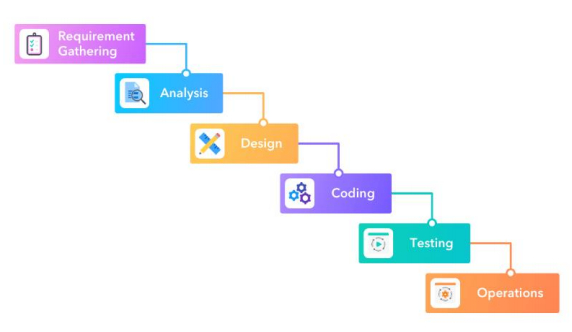
\includegraphics[width=0.5\linewidth]{figures/Week 3/Linear Approach.png}
\end{figure}

Traditionally, the approach to managing the lifecycle of a software application was a set of linear, sequential, stages that managed the development of the application as a project.

The waterfall method was typically used for this project management and was an earlier foundation of the PMBOK (Project Management body of Knowledge), and SDLC (Software Development Life Cycle) methodologies.

\subsubsection{Shift from Linear to Continuous}

\begin{table}[h]
\centering
\begin{tabular}{|c|c|}
\hline
\textbf{The Old model (Linear)}                                                                                     & \textbf{The New model (Continuous)}                                        \\ \hline
\begin{tabular}[c]{@{}c@{}}One way flow\\ Plan \textgreater Build \textgreater Deploy \textgreater End\end{tabular} & \begin{tabular}[c]{@{}c@{}}Ongoing\\ incremental improvements\end{tabular} \\ \hline
Large, infrequent releases.                                                                                         & Frequent, small releases                                                   \\ \hline
\end{tabular}
\end{table}

\noindent\textbf{Why the change?}

\begin{itemize}
    \item Need for agility in a fast-moving digital environment.
    \item Rising customer expectations for quick fixes and new features.
\end{itemize}

\bigskip

\noindent\textbf{Factors driving this shift}:

\begin{itemize}
    \item \textbf{Digital Transformation}: Need to keep pace with competitors.
    \item \textbf{Customer Expectations}: Users expect quick updates and fixes.
    \item \textbf{Cloud \& Automation}: Enables faster, safer deployments.
    \item \textbf{Agile \& DevOps Practices}: Promote collaboration and speed.
    \item \textbf{Data-Driven Decisions}: Continuous monitoring informs priorities.
\end{itemize}

\subsubsection{Continuous IT Lifecycle}

\begin{figure}[h]
    \centering
    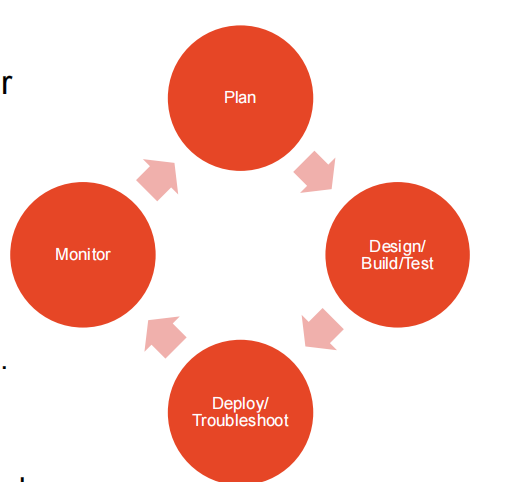
\includegraphics[width=0.5\linewidth]{figures/Week 3/Continuous IT Lifecycle.png}
\end{figure}

\noindent\textbf{Continuous IT Lifecycle}: A recurring, iterative approach to managing IT systems where improvement and delivery never stop. Instead of ending after deployment, IT work continues with \textbf{monitoring, feedback, and updates}. Enables faster innovation and responsiveness.

\bigskip

\noindent\textbf{Elements of the Continuous IT Lifecycle}:

\begin{itemize}
    \item Planning the development aligned with business strategy.
    \item Establishing the requirements, designing, building (or acquiring), testing.
    \item Deploying to the live environment (integrating with other e.g. other applications, middleware, operating systems), maintaining service levels (e.g. troubleshooting) and measuring performance
    \item Monitoring the value to the organisation. Depending on the results of the monitoring a new planning process would begin for refinements and improvements, making the cycle continuous (that cycle time can vary from very short to long)
\end{itemize}

\subsubsection{Linear Approach VS Continuous Approach}

\begin{table}[h]
\centering
\begin{tabular}{|c|c|l|}
\hline
\textbf{Aspect}                           & \textbf{Approach}                                                       &                                                                                                                                        \\ \hline
\multirow{2}{*}{\textbf{Definition}}      & \textbf{Linear}                                                         & \begin{tabular}[c]{@{}l@{}}A step-by-step,sequential method where each phase is\\ completed before moving to the next.\end{tabular}    \\ \cline{2-3} 
                                          & \textbf{\begin{tabular}[c]{@{}c@{}}Continuous\\ Lifecycle\end{tabular}} & \begin{tabular}[c]{@{}l@{}}A flexible,iterative approach where development,\\ testing,and deployment happen continuously.\end{tabular} \\ \hline
\multirow{2}{*}{\textbf{Process Flow}}    & \textbf{Linear}                                                         & \begin{tabular}[c]{@{}l@{}}One-way,structured progression\\ (e.g., Waterfall model).\end{tabular}                                      \\ \cline{2-3} 
                                          & \textbf{\begin{tabular}[c]{@{}c@{}}Continuous\\ Lifecycle\end{tabular}} & \begin{tabular}[c]{@{}l@{}}Cyclical and iterative,allowing feedback and\\ improvements(e.g., Agile, DevOps).\end{tabular}              \\ \hline
\multirow{2}{*}{\textbf{Flexibility}}     & \textbf{Linear}                                                         & \begin{tabular}[c]{@{}l@{}}Rigid-Changes are difficult to implement \\ once a phase is completed.\end{tabular}                         \\ \cline{2-3} 
                                          & \textbf{\begin{tabular}[c]{@{}c@{}}Continuous\\ Lifecycle\end{tabular}} & \begin{tabular}[c]{@{}l@{}}Highly adaptable-Continuous improvements \\ and iterations are possible.\end{tabular}                       \\ \hline
\multirow{2}{*}{\textbf{Risk Management}} & \textbf{Linear}                                                         & \begin{tabular}[c]{@{}l@{}}High risk-Issues are often detected\\ late in the process(e.g.,during testing).\end{tabular}                \\ \cline{2-3} 
                                          & \textbf{\begin{tabular}[c]{@{}c@{}}Continuous\\ Lifecycle\end{tabular}} & \begin{tabular}[c]{@{}l@{}}Lower risk-Continuous testing helps \\ identify and fix issues early.\end{tabular}                          \\ \hline
\multirow{2}{*}{\textbf{Examples}}        & \textbf{Linear}                                                         & \begin{tabular}[c]{@{}l@{}}Traditional software development,\\ large-scale enterprise systems, regulatory projects.\end{tabular}       \\ \cline{2-3} 
                                          & \textbf{\begin{tabular}[c]{@{}c@{}}Continuous\\ Lifecycle\end{tabular}} & \begin{tabular}[c]{@{}l@{}}Agile software development, DevOps,\\ cloud-based applications.\end{tabular}                                \\ \hline
\end{tabular}
\end{table}

\subsubsection{Metrics for Continuous IT Lifecycle Success}

\begin{table}[h]
\centering
\begin{tabular}{|c|l|}
\hline
\textbf{}                                 & \multicolumn{1}{c|}{\textbf{What it measures}}                                                                                                                                                         \\ \hline
\textbf{Release Frequency}                & \begin{tabular}[c]{@{}l@{}}How often new features, fixes, or updates are deployed.\\ (Example: Deploying updates every 2 weeks to add \\ new features in a university student portal.)\end{tabular}    \\ \hline
\textbf{Customer Satisfaction (CSAT/NPS)} & \begin{tabular}[c]{@{}l@{}}End-user satisfaction through surveys or Net Promoter Score.\\ (Example: Collecting feedback after each major \\ release of a mobile banking app.)\end{tabular}             \\ \hline
\textbf{Mean Time to Repair (MTTR)}       & \begin{tabular}[c]{@{}l@{}}Average time to resolve incidents or system outages.\\ (Example: Bringing a crashed e-learning platform back \\ online within 1 hour.)\end{tabular}                         \\ \hline
\textbf{Deployment Success Rate}          & \begin{tabular}[c]{@{}l@{}}Percentage of deployments that go live without rollback or issues.\\ (Example: Achieving 98\% success rate for cloud service \\ deployments without downtime.)\end{tabular} \\ \hline
\end{tabular}
\end{table}

\subsubsection{Common Pitfalls in Continuous Delivery}

\begin{itemize}
    \item \textbf{Over-automation without adequate testing}: Relying too heavily on automated pipelines without comprehensive automated and manual tests can lead to defects reaching production.
    \item \textbf{Insufficient stakeholder communication despite agile ceremonies}: Daily stand-ups, sprint reviews, and retrospectives can still fail if updates are superficial or key stakeholders are absent.
    \item \textbf{Security overlooked in rapid deployments}: Frequent releases can bypass thorough security checks, increasing vulnerabilities.
\end{itemize}

\subsection{Continuous IT lifecycle and Enterprise Architecture}

\subsubsection{Enterprise Architecture}

\noindent\textbf{Enterprise Architecture}: A structured framework for aligning an organisation’s business strategy, processes, information, and technology.

\bigskip

\noindent\textbf{Main Purpose}:

\begin{itemize}
    \item Ensure IT investments support business goals.
    \item Provide a blueprint for current and future systems.
\end{itemize}

\bigskip

\noindent\textbf{Core idea of an Enterprise}: Architecture is to bridge the gap between vision and execution.

\subsubsection{Why Enterprise Architecture matters?}

\begin{itemize}
    \item Strategic Alignment - Ensures IT and business priorities match.
    \item Efficiency - Reduces duplication and complexity.
    \item Agility - Enables quick adaptation to market changes.
    \item Risk Management - Identifies gaps and vulnerabilities in systems.
    \item Cost Optimisation - Avoids waste from overlapping tools or redundant processes.
\end{itemize}

\subsubsection{How does EA support Continuous delivery?}

\begin{itemize}
    \item Planning Phase - EA defines a roadmap for technology adoption and integration.
    \item Design \& Build Phase - EA standards ensure solutions fit into the broader organisational ecosystem.
    \item Deployment \& Monitoring - EA principles maintain interoperability and scalability.
    \item Feedback Loop - EA evolves as new business needs and technologies emerge.
\end{itemize}

\subsubsection{Key EA Components in Practice}

\begin{itemize}
    \item \textbf{Business Architecture}: Defines streamlined student enrolment workflows. Aligns services like course registration, fee payment, and academic records into a single process flow.
    \item \textbf{Application Architecture}: Integration of LMS (Canvas), CRM (Salesforce), and payment gateway through APIs
    \item \textbf{Data Architecture}: Centralised student database ensuring real-time updates across all systems.
    \item \textbf{Technology Architecture}: Cloud-based infrastructure for scalability. SSO (Single Sign-On) for all student-facing services
\end{itemize}

\subsubsection{Benefits of Enterprise Architecture}

\begin{itemize}
    \item Strategic Alignment - Ensures IT investments directly support business goals. Reduces the risk of "technology for technology’s sake".
    \item Improved Decision Making - Provides a holistic view of systems, processes, and data. Helps prioritise projects based on organisational value.
    \item Cost Optimisation - Reduces duplication of systems and services. Identifies under utilised resources and consolidates them.
    \item Risk Management - Identifies potential security, compliance, and operational risks early. Enables proactive planning for system upgrades or decommissioning.
    \item Better Collaboration - Breaks down silos between business and IT teams. Creates a common language for technical and non-technical stakeholders.
    \item Continuous Improvement Support - Works hand-in-hand with the Continuous IT Lifecycle to drive ongoing innovation and refinement.
\end{itemize}

\subsection{Question}

\subsubsection{End of lecture questions}

\begin{itemize}
    \item In your own words, how does the continuous IT lifecycle differ from the traditional linear approach?
    \item Why might an organisation choose Agile over Waterfall, or DevOps over both?
    \item How can enterprise architecture help avoid project failures?
    \item How could EA frameworks like TOGAF or Zachman be applied to support continuous improvement?
    \item Think of an IT project you have studied. Which lifecycle stages were the most challenging, and why?
\end{itemize}

\subsubsection{Case-study based Questions}

\noindent\textbf{Company}: HealthLink Systems (Fictional Healthcare Software Provider)

\noindent\textbf{Background}:
\begin{itemize}
    \item HealthLink provides hospital management software used by over 200 hospitals.
    \item Faced frequent delays in software updates due to siloed business and IT teams.
    \item Customer feedback indicated dissatisfaction with long wait times for bug fixes and feature updates.
\end{itemize}

HealthLink Systems shifted from a Waterfall delivery model to a Continuous IT Lifecycle supported by TOGAF-based Enterprise Architecture. They achieved faster releases, reduced costs, and improved customer satisfaction.

\bigskip

\noindent\textbf{Question}:

\begin{itemize}
    \item Which three major issues did HealthLink face before the shift?
    \item Why was moving to a continuous IT lifecycle more suitable than keeping the linear approach?
    \item Would Agile alone have solved their problems, or was DevOps also necessary? Explain.
    \item How did EA contribute to the long-term success of the transformation?
    \item If HealthLink wanted to add AI-based predictive analytics for hospitals, how would EA ensure its smooth integration?
\end{itemize}
\pagebreak

\section{Week 4 - Professional communication, Collaboration and Stakeholder Management}
\subsection{Communication}

\indent 

\noindent\textbf{Communication ensure alignment between}:

\begin{itemize}
    \item Developers, testers, project managers
    \item Clients, users, external, stakeholders
\end{itemize}

\bigskip

\noindent\textbf{Types of Communication in IT projects}:

\begin{itemize}
    \item Written
    \item Verbal
    \item Presentation/Visual
    \item Non-verbal
\end{itemize}

\subsubsection{Communication in IT}

\indent 

IT Projects are collaborative and multidisciplinary.

\noindent\textbf{Communication in IT is critical for}:

\begin{itemize}
    \item Requirement Gathering
    \item Team Coordination
    \item Stakeholder Engagement
    \item Reporting Progress
\end{itemize}

\subsubsection{Written Communication}

\indent 

\noindent\textbf{Formal}:Emails, Reports, Contracts, Documentations, etc.

\noindent\textbf{Informal}: Slack chats, Shared Notes, etc.

\noindent\textbf{Best practices}: Be clear and concise; Avoid jargon unless necessary; Proofread before sending.

\subsubsection{Verbal Communication}

\indent 

Face-to-face, virtual meetings, stand-ups.

\noindent\textbf{Benefits}: Quick clarification, Builds trust.

\noindent\textbf{Skills needed}: Active listening, Speaking with clarity, Managing tone and pace.

\noindent\textbf{Pitfalls}: Dominance of few voices, missed follow-ups.

\subsubsection{Presentations}

\indent 

\noindent\textbf{Used for}: Project proposals, Stakeholder updates, Demos, etc.

\bigskip

\noindent\textbf{Key elements}:

\begin{itemize}
    \item Story telling (Problem $\Longrightarrow$ Solution $\Longrightarrow$ Impact)
    \item Visual Aids (Charts, Diagrams, Dashboards)
    \item Audience Awareness (Technical vs Non-technical)
\end{itemize}

\subsubsection{Effective Communication Frameworks}

\indent 

\noindent\textbf{7Cs of Communication}

\begin{itemize}
    \item \textbf{Clear}: Message should be easy to understand and avoid vague language
    \item \textbf{Concise}: Keep it short and to the point, avoid unnecessary details.
    \item \textbf{Concrete}: Use specific facts, data, or example rather than abstract statements.
    \item \textbf{Correct}: Ensure information is accurate and error free (grammar, spelling, etc.)
    \item \textbf{Coherent}: Message should be logical, well structured, and flow naturally.
    \item \textbf{Complete}: Provide all necessary information so there are no follow-up questions.
    \item \textbf{Courteous}: Be respectful, positive, and polite. Encourage collaboration.
\end{itemize}

\bigskip

\noindent\textbf{SBAR Framework}

\begin{itemize}
    \item \textbf{Situation}: State the immediate issue/problem clearly and briefly. What is happening right now?
    \item \textbf{Background}: Provide context or relevant history. What led to this issue? Why is it important?
    \item \textbf{Assessment}: Share your analysis or findings. What do you think is the cause? What is the impact?
    \item \textbf{Recommendation}: Propose next steps or actions to be taken. Clearly state what you need from the other person.
\end{itemize}

\subsubsection{Barriers to communication in IT Teams}

\begin{itemize}
    \item Technical jargon/acronyms
    \item Cultural and Language differences
    \item Remote collaboration challenges (time zones, etc.)
    \item Assumptions and lack of active listening
    \item Poor documentation >>> Knowledge gaps
\end{itemize}

\subsection{Teamwork}

\subsubsection{Importance of teamwork}

\indent 

IT projects are collaborative in nature.

Combines diverse expertise (developers, testers, designers, managers, 
business analysts)

\noindent\textbf{Teamwork leads to}:

\begin{itemize}
    \item Faster problem-solving
    \item Higher creativity \& innovation
    \item Shared responsibility \& accountability
    \item Stronger project outcomes
\end{itemize}

\bigskip 

\noindent\textbf{An effective IT Team}:

\begin{itemize}
    \item Clear roles \& responsibilities
    \item Trust \& psychological safety
    \item Open and respectful communication
    \item Shared goals and accountability
    \item Ability to adapt to change
    \item Balance of technical and soft skills
\end{itemize}

\subsubsection{Mistaken beliefs about teamwork}

\begin{itemize}
    \item “Teamwork means everyone has to agree” $\Longrightarrow$ \textbf{No, healthy disagreements drive better outcomes}
    \item “Teamwork slows things down” $\Longrightarrow$ \textbf{Actually, collaboration reduces rework and errors}
    \item “Good teams don’t have conflicts” $\Longrightarrow$ \textbf{Conflicts are normal; it’s how they’re resolved that matters}
    \item “Teamwork means equal contribution from all” $\Longrightarrow$ \textbf{Different roles contribute in different ways}
\end{itemize}

\subsubsection{Teamwork and Diversity}

\indent 

\noindent\textbf{Types of Diversity}:

\begin{itemize}
    \item Cultural and linguistic
    \item Educational and technical background
    \item Gender, age, and experiences
\end{itemize}

\bigskip

\noindent\textbf{Pros}: better problem-solving, user-centered products, broader perspectives, more innovation.

\noindent\textbf{Challenges}: communication barriers, unconscious bias.

\bigskip

\noindent\textbf{Team dynamics and Challenges}:

\begin{itemize}
    \item Unequal participation
    \item Dominant personalities vs quiet contributors
    \item Misaligned goals or unclear expectations
    \item Cross-cultural misunderstandings
    \item Remote/virtual team challenges (time zones, engagement)
\end{itemize}

\subsubsection{Belbin's Team Roles}

\indent 

\noindent\textbf{What are Belbin's Team roles?}

A framework developed by Dr. Meredith Belbin to identify nine behavioral roles 
people adopt in teams. Helps create balanced teams by ensuring all critical roles are covered. Roles are grouped into three categories: Social, Thinking, and Action/Task.

\bigskip

\noindent\textbf{Nine roles}:

\begin{itemize}
    \item \textbf{Social}: Resource Investigator, Team-worker, Coordinator
    \item \textbf{Thinking}: Plant, Monitor Evaluator, Specialist
    \item \textbf{Action/Task}: Shaper, Implementer, Completer Finisher
\end{itemize}

\bigskip

\noindent\textbf{Why does it matter?}

\begin{itemize}
    \item Encourages awareness of strengths and weaknesses.
    \item Prevents role overlap or gaps.
    \item Supports better teamwork and project outcomes.
\end{itemize}

\subsubsection{Psychological Safety – Google’s Project Aristotle}

\indent 

\noindent\textbf{What is Psychological safety?}

Shared belief that team members can take risks without fear of embarrassment 
or punishment. Encourages open communication, idea sharing, and learning from mistakes. Key driver of trust and collaboration in high-performing teams.

\bigskip

\noindent\textbf{Why it matters in IT projects?}

\begin{itemize}
    \item Promotes innovation and creativity.
    \item Reduces fear of speaking up about errors, leading to fewer failures.
    \item Improves engagement, morale, and resilience under pressure.
\end{itemize}

\bigskip

\noindent\textbf{How to create it?}

\begin{itemize}
    \item \textbf{Encourage curiosity}: Value questions and new ideas.
    \item \textbf{Normalize mistakes}: Treat errors as opportunities to learn.
    \item \textbf{Active listening}: Leaders and peers listen without judgment.
    \item \textbf{Inclusive environment}: Ensure all voices are heard, not just dominant ones.
    \item \textbf{Clear expectations}: Define roles, but allow flexibility for contributions.
\end{itemize}

\bigskip

\noindent\textbf{Impact on Teams}

\begin{itemize}
    \item Higher innovation and creativity.
    \item Faster problem-solving and adaptability.
    \item Stronger sense of belonging and collaboration
\end{itemize}

\subsubsection{Agile Teamwork Practices}

\begin{itemize}
    \item \textbf{Daily Standup}: Usually a daily meeting, lasting no more than 15 minutes. Team members describe what they worked in the previous day, and what are they intend to work on today. It should not be detailed.
    \item \textbf{Sprint Planning}: The team uses this meeting to decide what to do during the sprint.
    \item \textbf{Sprint Review}: At the end of a sprint or milestone, the team reviews their accomplishments against the planned sprint work. The team will often use this meeting to demonstrate the results of their work and get feedback from stakeholders.
    \item \textbf{Sprint Retrospective}: At the end of an iteration, the team discusses what worked well, and what could be improved.
\end{itemize}

\subsubsection{Conflicts in the Workplace}

\indent 

\noindent\textbf{Common Sources}

\begin{itemize}
    \item Competing priorities
    \item Miscommunication
    \item Personality clashes
    \item Ambiguous responsibilities
    \item Resource constraints
\end{itemize}

\bigskip

\noindent\textbf{Impact if unmanaged}

\begin{itemize}
    \item Reduced productivity
    \item Low morale
    \item Stakeholder dissatisfaction
\end{itemize}

\subsubsection{Task Conflict VS Relationship Conflict}

\indent 

\noindent\textbf{Task conflict (Cognitive conflict)}

\begin{itemize}
    \item Disagreements about \textbf{work-related issues} (goals, ideas, processes, tasks).
    \item Can be constructive, stimulates critical thinking, innovation, and better decisions.
\end{itemize}

\bigskip

\noindent\textbf{Relationship conflict (Affective conflict)}

\begin{itemize}
    \item Based on \textbf{personal incompatibilities} (personality clashes, tension, mistrust).
    \item Usually \textbf{destructive}, reduces team cohesion, satisfaction, and performance.
\end{itemize}

\subsection{Stakeholder Management}

\indent

\noindent\textbf{Who are stakeholders?}

Individuals, groups, or organizations affected by or having an interest in the project.

\bigskip

\noindent\textbf{Why does stakeholder management matter?}

\begin{itemize}
    \item Aligns expectations with deliverables
    \item Minimizes conflict and scope creep
    \item Builds trust and project credibility
\end{itemize}

\subsubsection{Stakeholder analysis and mapping}

\indent 

The main purpose of this step is to understand stakeholder needs, interests, and influence.

\noindent\textbf{The major steps for stakeholder analysis and mapping are}:

\begin{itemize}
    \item Identify stakeholders (internal \& external)
    \item Assess their interests, expectations, and influence
    \item Prioritize based on their importance
    \item Develop tailored engagement strategies
\end{itemize}

\bigskip

\noindent\textbf{Power Interest Matrix}: This is a tool to categorize the 
stakeholders by Power (ability to influence the project) \& Interest (level of concern or involvement). Helps decide how much time and effort to invest in managing each stakeholder.

\begin{figure}[h]
    \centering
    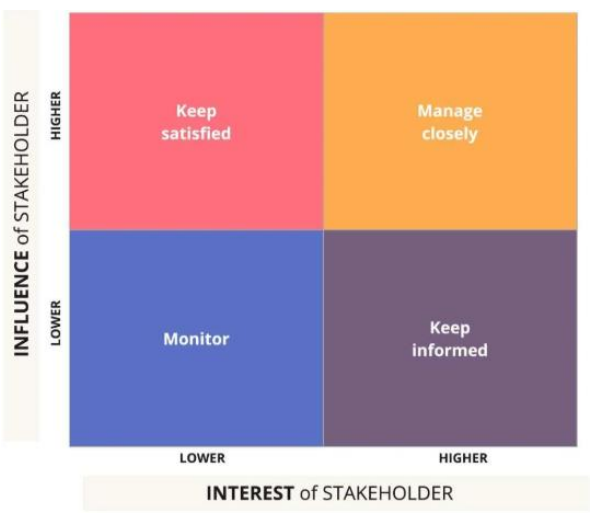
\includegraphics[width=0.5\linewidth]{figures/Week 4/Power Interest Matrix.png}
\end{figure}

\bigskip

\noindent\textbf{Salience Model}: An advanced stakeholder analysis tool. Categorises stakeholders based on 3 attributes: Power (ability to influence), Legitimacy: (appropriateness of their involvement), Urgency (how quickly they require attention)

\begin{figure}[h]
    \centering
    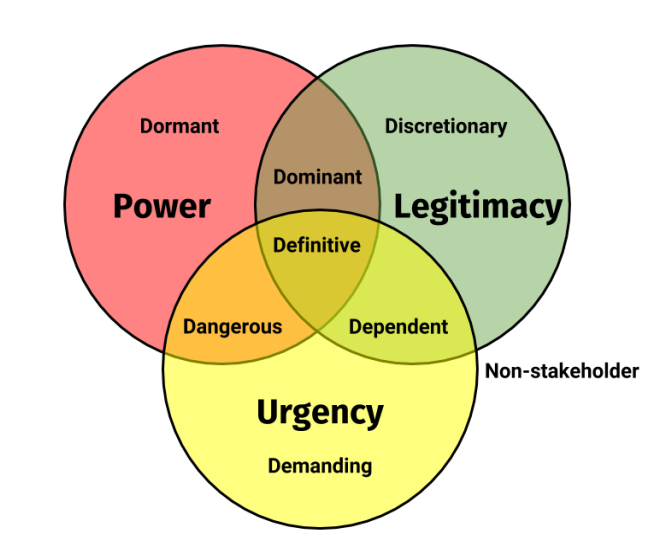
\includegraphics[width=0.5\linewidth]{figures/Week 4/Salience Model.png}
\end{figure}

\begin{itemize}
    \item \textbf{Definitive (Power + Legitimacy + Urgency)}: Highest priority
    \item \textbf{Dominant (Power + Legitimacy)}: Strong influence, need active management
    \item \textbf{Dependent (Legitimacy + Urgency)}: Need support to gain power (e.g., end-users)
    \item \textbf{Dangerous (Power + Urgency)}: Can disrupt if ignored
    \item \textbf{Dormant (Power only)}: Potential influence if mobilized
    \item \textbf{Discretionary (Legitimacy only)}: Low involvement, can support reputation
    \item \textbf{Demanding (Urgency only)}: Attention-seeking, but low impact
\end{itemize}

\subsubsection{Engagement strategies}

\indent 

One must match the strategy to the stakeholder category. There are several levels of engagement:

\begin{itemize}
    \item \textbf{Inform}: Low power, low interest → newsletters, emails
    \item \textbf{Consult}: Seek input from those affected
    \item \textbf{Involve}: Engage in workshops, feedback sessions
    \item \textbf{Collaborate}: Co-create solutions, joint decision-making
    \item \textbf{Empower}: Give decision-making authority (e.g., product owners in Agile)
\end{itemize}

Use multiple channels: reports, demos, townhalls, dashboards.

\subsubsection{Challenges in Stakeholder Management}

\begin{itemize}
    \item Changing requirements during project lifecycle
    \item Conflicting interests between stakeholder groups
    \item Cultural/language barriers (global IT teams)
    \item Stakeholders with unrealistic expectations
    \item Hidden stakeholders not identified early
    \item Over- or under-communicating with certain groups
\end{itemize}

\subsubsection{Best practices}

\begin{itemize}
    \item Start stakeholder analysis \textbf{early} and update regularly
    \item Use \textbf{clear communication frameworks} (7Cs, SBAR)
    \item Manage expectations $\Longrightarrow$ under-promise, over-deliver
    \item Foster \textbf{trust and transparency}
    \item Document decisions \& agreements
    \item Balance time spent across stakeholder groups (don’t neglect “low power, high interest” users)
    \item Regular engagement $\Longrightarrow$ reviews, feedback loops, demos
\end{itemize}

\subsection{How does it all come together?}

\indent 

\noindent\textbf{Interconnected nature}:

\begin{itemize}
    \item Communication is the \textbf{glue}: ensures clarity between team members and stakeholders.
    \item Teamwork is the \textbf{engine}: drives collaboration, innovation, and delivery.
    \item Stakeholder Management is the \textbf{direction}: ensures the team is building the right thing, aligned with expectations.
\end{itemize}

\bigskip

\noindent\textbf{Why can't each of these 3 work in isolation?}

\begin{itemize}
    \item Poor communication $\Longrightarrow$ teamwork suffers, stakeholders lose trust.
    \item Poor teamwork $\Longrightarrow$ communication breaks down, deliverables slip.
    \item Poor stakeholder management $\Longrightarrow$ even a strong team delivering great work risks rejection if it doesn’t meet stakeholder needs.
\end{itemize}

\subsection{Question}

\subsubsection{End of Lecture Questions}

\begin{itemize}
    \item What are the 7 Cs of Communication, and why are they important in IT projects?
    \item According to Tuckman’s model, what typically happens during the “Storming” stage of team development?
    \item What are some conflict resolution strategies, and when might you use them?
    \item What are two common challenges in stakeholder management, and how can they be addressed?
    \item Compare the Power–Interest Matrix and the Salience Model. How do they differ in analyzing stakeholders?
    \item How do communication, teamwork, and stakeholder management work together to ensure IT project success?
\end{itemize}

\subsubsection{Case Study}

\indent

A software company is developing a mobile banking app for a major bank.

\noindent\textbf{Stakeholders}: The bank’s executives (sponsors), compliance officers (regulators), customer support staff, IT developers, and end-users (customers).

\noindent\textbf{Situation}:

\begin{itemize}
    \item During development, developers find conflicting requirements from executives (wanting faster release) and compliance officers (demanding more security checks).
    \item The team also faces internal conflict: testers complain that developers don’t provide enough documentation, while developers argue that deadlines are too tight.
    \item The client complains about unclear updates, saying they’re “not sure what’s really happening with the project.”
\end{itemize}

\bigskip

\noindent\textbf{Question}:

\begin{itemize}
    \item Identify at least two communication failures in this scenario.
    \item Which stage of Tuckman’s model does this team appear to be in? Why?
    \item What conflict resolution strategy would you apply between developers and testers?
    \item Place the executives, compliance officers, and end-users into the Power–Interest Matrix.
    \item How can better communication, teamwork, and stakeholder management together prevent project delays in this scenario?
\end{itemize}
\pagebreak

\section{Week 5 - Evidence based practice and Estimation for IT projects}
\subsection{Information}

\indent 

\noindent \textbf{Information}: Collection of data that can be processed, organised, and structured in a meaningful way to convey knowledge, ideas, or instructions.

\bigskip

\noindent Why is \textbf{information important} in IT Professional Practice?

\begin{itemize}
    \item Decision making
    \item Communication with stakeholders
    \item Problem solving and troubleshooting
    \item Project management
    \item Knowledge sharing and continuous learning
    \item Compliance and Ethics
\end{itemize}

\subsubsection{DIKW Hierarchy}

\begin{figure}[h]
    \centering
    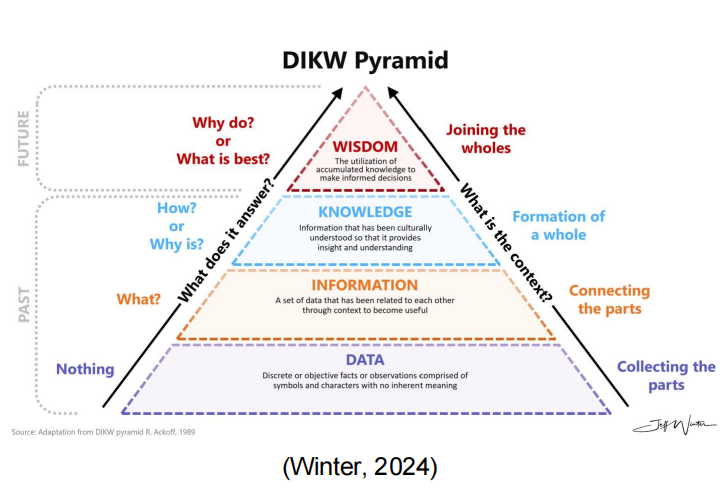
\includegraphics[width=0.7\linewidth]{figures/Week 5/DIKW.png}
\end{figure}

\noindent\textbf{Data}: Raw facts, figures, or symbols without context.

\noindent\textbf{Information}: Processed or organized data that has meaning.

\noindent\textbf{Knowledge}: Applying experience, context, and interpretation to information.

\noindent\textbf{Wisdom}: The ability to make sound judgments and decisions using knowledge.

\subsubsection{What level of information/knowledge is needed?}

\indent 

\noindent\textbf{Data Level}: Needed by technical specialists (e.g., programmers, system admins, analysts) to work with raw logs, records, metrics.

\noindent\textbf{Information Level}: Needed by IT professionals across all roles for decision-making, communication, and reporting. This is the minimum level expected in professional IT practice.

\noindent\textbf{Knowledge Level}: Needed by project managers, consultants, business analysts, senior engineers to interpret and apply information.

\noindent\textbf{Wisdom Level}: Needed by leaders, strategists, architects, and executives for long-term, ethical, and strategic decision-making.

\subsubsection{Why credible information is important?}

\indent 

Credible information is necessary because it ensures \textbf{trustworthy decisions, ethical practice, compliance with laws, and professional accountability}. Without credibility, information loses its value and can even cause harm.

\begin{itemize}
    \item \textbf{Accuracy in Decision}: making Decisions are only as good as the information behind them. Inaccurate or misleading information can lead to costly mistakes, failed projects, or security risks.
    \item \textbf{Trust and professional reputation}: IT professionals work with clients, managers, and users who depend on them. Sharing credible, evidence-based information builds trust and strengthens professional reputation.
    \item \textbf{Risk reduction}: Credible information helps identify risks correctly and avoid poor choices
    \item \textbf{Compliance and Ethics}: Many industries (healthcare, finance, government) require IT professionals to handle verified, accurate information for legal and ethical reasons. Using non-credible information can result in legal breaches, data leaks, or loss of privacy.
    \item \textbf{Efficient Communication}: Teams and stakeholders need a common, reliable source of truth. Credible information ensures everyone is aligned, reducing conflict and confusion.
\end{itemize}

\subsubsection{Sources of Information}

\begin{itemize}
    \item Primary Sources.
    \begin{itemize}
        \item Direct, original, or firsthand evidence.
        \item Example: Research reports, surveys, interviews, company records \& logs, etc
    \end{itemize}
    \item Secondary Sources
    \begin{itemize}
        \item Interpretations, summaries, or analyses of primary data.
        \item Example: Textbooks, documentations, industry reports, news articles, etc.
    \end{itemize}
    \item Tertiary Sources
    \begin{itemize}
        \item Consolidated collections of primary and secondary sources.
        \item Example: Encyclopedias, dictionaries, databases, etc.
    \end{itemize}
\end{itemize}

\subsubsection{Information usefulness vs uselessness}

\indent

\noindent\textbf{Useful Information}: Accurate, Relevant, Timely, Complete, Credible, Understandable, Actionable.

\noindent\textbf{Useless Information}: Inaccurate, Irrelevant, Outdated, Incomplete, Redundant, Unverifiable, Ambiguous.

\subsubsection{What level of information validity is needed?}

\indent

\noindent\textbf{Validity}: The extent to which information is accurate, reliable, and 
represents reality correctly.

\begin{itemize}
    \item \textbf{High} Validity (Critical contexts): Needed when mistakes have serious consequences (legal, financial, ethical, or safety). Example: Medical records, Cybersecurity threat alerts.
    \item \textbf{Moderate} Validity (Operational contexts): Needed for day-to-day IT operations where minor errors can be tolerated but should still be minimized. Example: Project progress reports.
    \item \textbf{Low} Validity (Exploratory/Informal Contexts): Acceptable when using information for brainstorming, trend analysis, or innovation where approximate accuracy is fine. Example: feedback surveys.
\end{itemize}

\subsubsection{How to find information effectively?}

\indent 

\step Define the need: Be clear about what you are looking for.

\step Choose the right sources.

\step Use effective search strategies: Use keywords + Boolean operators (AND, OR, NOT).

\step Evaluate credibility: Use the CRAAP test.

\step Organise and store information: Use reference managers (Zotero, Mendeley, EndNote) and keep structured notes (Evernote, Notion, OneNote)

\step Apply and communicate: Turn raw information into insightful reports, dashboards, or recommendations. Ensure clarity so others can trust and use the information

\subsubsection{CRAAP Test}

\begin{figure}
    \centering
    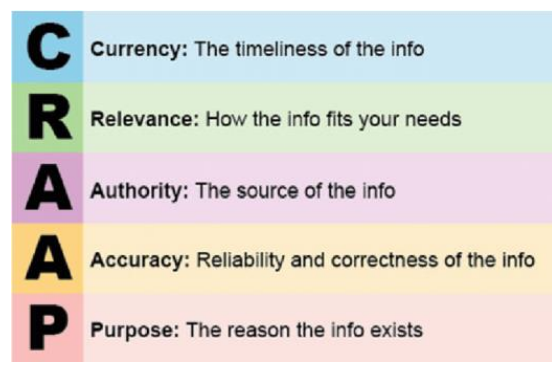
\includegraphics[width=0.7\linewidth]{figures/Week 5/CRAAP.png}
\end{figure}

\begin{itemize}
    \item \textbf{Currency}: Is the information up to date? When was it published or updated?
    \item \textbf{Relevance}: Does the information directly relate to your question or problem? Is it at the right level (too simple / too advanced)?
    \item \textbf{Authority}: Who is the author, publisher, or organization? Are they recognized experts?
    \item \textbf{Accuracy}: Is the information supported by evidence, references, or data? Has it been peer-reviewed or tested?
    \item \textbf{Purpose}: Why was this information created? To inform, teach, sell, persuade, entertain? Is there bias or hidden agenda?
\end{itemize}

\subsubsection{Referencing sources of Information}

\indent

Referencing is how you give credit to the sources of information you’ve used. In IT professional practice and academia, referencing is essential to: 

\begin{itemize}
    \item \textbf{Acknowledge authorship}: avoiding plagiarism.
    \item \textbf{Support credibility}: showing your info is backed by evidence.
    \item \textbf{Allow verification}: so others can find the original source.
\end{itemize}

Common Referencing styles:

\begin{itemize}
    \item \textbf{APA}: Common in IT \& Social Sciences. We use the APA7 format for the assignment.
    \item \textbf{Harvard}: Widely used across disciplines.
    \item \textbf{IEEE}: Standard in engineering, computer science, IT.
\end{itemize}

\subsection{Research}

\indent 

\noindent\textbf{Research}: a systematic process of collecting, analyzing, and interpreting information (data) to answer questions, solve problems, or generate new knowledge.

\bigskip

\noindent Key characteristics:

\begin{itemize}
    \item \textbf{Systematic}: Follows a clear method or process (not random searching).
    \item \textbf{Objective}: Seeks truth or valid results, avoiding personal bias.
    \item \textbf{Evidence based}: Relies on data, experiments, or credible sources.
    \item \textbf{Replicable}: Others should be able to follow the process and reach similar results.
    \item \textbf{Innovative}: Often aimed at discovering new insights or improving existing ones.
\end{itemize}

\subsubsection{Types of Research}

\begin{itemize}
    \item Pure Research: Expands theoretical knowledge (e.g., algorithms, AI models).
    \item Applied Research: Solves practical problems (e.g., developing an HRMS system).
    \item Qualitative Research: Focuses on non-numerical insights (e.g., user experience studies).
    \item Quantitative Research: Uses measurable, numerical data (e.g., system performance benchmarks).
\end{itemize}

\subsubsection{Why research is important in IT?}

\begin{itemize}
    \item \textbf{Innovation and Advancement}: IT evolves rapidly (AI, cloud, cybersecurity, IoT, blockchain). Research drives new technologies, methods, and tools, ensuring professionals stay ahead.
    \item \textbf{Problem Solving}: Research provides systematic approaches to analyze and solve technical or business challenges.
    \item \textbf{Evidence based Decision Making}: Research ensures IT strategies are based on facts, data, and evidence, not assumptions.
    \item \textbf{Improving Professional Practice}: Research identifies best practices, standards, and methodologies (e.g., Agile, ITIL, DevOps).
\end{itemize}

\subsubsection{Primary Research vs Secondary Research}

% Please add the following required packages to your document preamble:
% \usepackage[normalem]{ulem}
% \useunder{\uline}{\ul}{}
\begin{table}[h]
\centering
\begin{tabular}{|c|l|lll|}
\hline
\textbf{Feature}       & \multicolumn{1}{c|}{\textbf{Primary Research}}                                                                                                    & \multicolumn{3}{c|}{\textbf{Secondary Research}}                                                                                                                                  \\ \hline
\textbf{Definition}    & \begin{tabular}[c]{@{}l@{}}Collection of original, first-hand \\ data directly from sources.\end{tabular}                                         & \multicolumn{3}{l|}{\begin{tabular}[c]{@{}l@{}}Use of existing data or information \\ collected by others.\end{tabular}}                                                          \\ \hline
\textbf{Purpose}       & \begin{tabular}[c]{@{}l@{}}To answer specific research \\ questions or problems.\end{tabular}                                                     & \multicolumn{3}{l|}{\begin{tabular}[c]{@{}l@{}}To gather background information,\\ support analysis, or compare findings.\end{tabular}}                                           \\ \hline
\textbf{Sources}       & \begin{tabular}[c]{@{}l@{}}Surveys, interviews, observations,\\ experiments, system logs.\end{tabular}                                            & \multicolumn{3}{l|}{\begin{tabular}[c]{@{}l@{}}Books, journal articles, industry reports,\\ websites, databases.\end{tabular}}                                                    \\ \hline
\textbf{Advantages}    & \begin{tabular}[c]{@{}l@{}}Tailored to your specific research \\ question.\\ Up-to-date and specific.\\ Direct control over quality.\end{tabular} & \multicolumn{3}{l|}{\begin{tabular}[c]{@{}l@{}}Saves time and resources.\\ Provides a broader perspective.\\ Useful for trend analysis and background \\ knowledge.\end{tabular}} \\ \hline
\textbf{Disadvantages} & \begin{tabular}[c]{@{}l@{}}Time-consuming and costly.\\ Requires careful planning and \\ execution.\end{tabular}                                  & \multicolumn{3}{l|}{\begin{tabular}[c]{@{}l@{}}May not be fully relevant or up-to-date.\\ Dependent on the credibility of the \\ original source.\end{tabular}}                   \\ \hline
\textbf{Examples}      & \begin{tabular}[c]{@{}l@{}}Conducting a user survey to test \\ a new HRMS interface.\end{tabular}                                                 & \multicolumn{3}{l|}{\begin{tabular}[c]{@{}l@{}}Reviewing IEEE papers or Gartner reports\\ to learn about cloud security trends.\end{tabular}}                                     \\ \hline
\end{tabular}
\end{table}

\subsubsection{Why statistics matter for research in IT?}

\begin{itemize}
    \item \textbf{Making sense of the Data}: IT research often involves large volumes of data (system logs, user surveys, performance metrics). Statistics provide the tools to analyze, summarize, and interpret this data meaningfully.
    \item \textbf{Turning data into information}: Raw data (primary research) becomes information only when analyzed. Statistics help transform raw counts and numbers into patterns, correlations, and insights.
    \item \textbf{Evidence based decisions}: In IT, decisions about system design, project feasibility, or security risks must be evidence-based. Statistical tests confirm whether findings are valid, reliable, and significant
\end{itemize}

\subsubsection{Important concepts in statistics}

\indent 

\noindent\textbf{Population}: The complete set of items/people/data you are studying.

\noindent\textbf{Sample}: A subset of the population used to make inferences.

\noindent\textbf{Quantitative (Numerical)}: Can be measured and expressed as numbers (e.g., response time, CPU usage).

\noindent\textbf{Qualitative (Categorical)}: Non-numeric, describes qualities (e.g., OS type: Windows, macOS, Linux).

\noindent\textbf{Descriptive}: Summarises data (e.g., mean, median, charts).

\noindent\textbf{Inferential}: Makes predictions or conclusions from data (e.g., hypothesis testing, confidence intervals).

\noindent\textbf{Mean}: Average value.

\noindent\textbf{Median}: Middle value.

\noindent\textbf{Mode}: Most frequent value.

\noindent\textbf{Range}: Difference between max and min.

\noindent\textbf{Variance/Standard Deviation}: How much data points deviate from the mean.

\noindent\textbf{Probability}: The likelihood of an event occurring. Useful in IT for risk assessment, machine learning, and predictive analytics.

\noindent\textbf{Correlation}: : Two variables move together (e.g., internet speed $\uparrow$, user satisfaction $\uparrow$).

\noindent\textbf{Causation}: One variable directly influences another (requires deeper research).

\subsection{Estimation}

\indent 

\noindent\textbf{Estimation}: the process of predicting the effort, time, cost, and resources needed to complete a project or task before the actual work begins.

\bigskip

In IT, estimation is often applied to software development, system implementation, testing, and infrastructure setup.

\subsubsection{Importance of Estimation for IT projects}

\indent

\noindent\textbf{Project Planning \& Scheduling}: 

Accurate estimates allow project managers to plan timelines, set milestones, and allocate resources effectively. Without estimation, projects risk delays and bottlenecks.

\bigskip

\noindent\textbf{Budgeting \& Cost Control}:

Organizations need to forecast project costs for approval and funding. Estimation ensures that financial resources are not over- or under-allocated.

\bigskip

\noindent\textbf{Stakeholder Expectations}:

Helps set realistic deadlines and deliverables for clients, sponsors, and team 
members. Builds trust with stakeholders through transparency.

\bigskip

\noindent\textbf{Resource Management}:

Ensures that human resources (developers, testers, analysts) and technical resources (servers, licenses, tools) are allocated efficiently.

\bigskip

\noindent\textbf{Risk Management}:

Identifies possible overruns early thereby allowing teams to prepare contingency plans.

\bigskip\textbf{Performance Measurement}:

Actual project performance can be compared with estimates to improve future forecasting accuracy.

\subsubsection{5 Steps in Project Estimation}

\indent

\step Determine the \textbf{SIZE} of the project.

This means defining the project scope, functionality, and complexity. In IT, size can be measured using methods like function points, story points, lines of code (LOC), or number of features.

\step Determine the \textbf{EFFORT} required

Effort refers to the total work needed to complete the project. This is typically measured in person-hours, person-days, or person-months. Tools like COCOMO (Constructive Cost Model) or agile estimation techniques can be applied.

\step Decide on the \textbf{RESOURCES} needed

Resources include human (developers, testers, designers), technical (software, hardware, tools), and financial resources. Allocation depends on skill sets required and availability.

\step Calculate the \textbf{DURATION}

Duration is the calendar time required to finish the project given the available resources and effort. Effort and duration are not the same: 100 hours of effort could take 2 weeks with one developer or 1 week with two developers.

\step Calculate the \textbf{COST}

\begin{align*}
    \text{Cost} = (\text{Effort}\times \text{Resource rate}) + \text{Overheads (infrastructure, tools, licenses, etc.)}
\end{align*}

Helps in budgeting and client negotiations.

\subsubsection{5 Approaches to Project Estimation}

\indent 

\noindent\textbf{Function Point Analysis (FPA)}:

Estimates project size by counting the number of “functions” the system must perform (inputs, outputs, user interactions, files, interfaces). Each is given a weight (simple, average, complex).

Good for estimating software development effort where requirements are well-defined.

\bigskip

\noindent\textbf{Algorithmic Cost Models}:

Uses mathematical models based on historical data to estimate effort, cost, and duration. The most famous is COCOMO (Constructive Cost Model).

Usually used in large projects with measurable code size (KLOC = thousands of lines of code).

\bigskip

\noindent\textbf{Expert Judgement}: 

Relies on experienced IT professionals to give estimates based on past-experience.

Used in early-stage projects with uncertain requirements.

\bigskip

\noindent\textbf{Estimation by Analogy}

Compares the project with a similar past project and adjusts based on differences.

Best used when historical projects are available as benchmarks.

\bigskip

\noindent\textbf{Sum of parts}

Breaks the project into tasks or subtasks (like a WBS – Work Breakdown Structure). Each task is estimated separately, then summed up.

Best for detailed project planning when tasks are well-defined.

\subsubsection{Limitations and Biases in Estimation Methods}

\indent 

\noindent\textbf{Function Point Analysis (FPA)}:

\textbf{Limitations}: Can be time-consuming; requires detailed functional specifications early on (which may not always be available).

\textbf{Biases}: Depends on the estimator’s interpretation of system complexity. Different evaluators may assign different function point values.

\bigskip

\noindent\textbf{Algorithmic Cost Models}:

\textbf{Limitations}: Based on assumptions and calibration with historical data; less accurate for novel or emerging technologies.

\textbf{Biases}: “Garbage in, garbage out” - biased or poor-quality input data leads to inaccurate results.

\bigskip

\noindent\textbf{Expert Judgement}: 

\textbf{Limitations}: Relies heavily on personal experience; may not scale well for large, complex projects.

\textbf{Biases}: Subjective optimism (underestimating effort) or pessimism (overestimating effort). Experts may also anchor on past projects that don’t exactly match the current one.

\bigskip

\noindent\textbf{Estimation by Analogy}

\textbf{Limitations}: Requires good historical project data that is truly comparable; differences in scope/technology may be overlooked.

\textbf{Biases}: Over-reliance on similarities, ignoring unique aspects of the new project. May cause “false equivalence bias.”

\bigskip

\noindent\textbf{Sum of parts}

\textbf{Limitations}: Risk of double-counting effort or overlooking hidden dependencies between components

\textbf{Biases}: Anchoring bias if estimators fixate on certain parts while ignoring integration overheads.

\subsubsection{Agile vs Traditional Estimation}

\begin{table}[h]
\centering
\begin{tabular}{|c|l|ll|}
\hline
\textbf{Aspect}      & \multicolumn{1}{c|}{\textbf{Agile Estimation}}                                                                                                                                                                     & \multicolumn{2}{c|}{\textbf{Traditional Estimation}}                                                                                                                                                                                                          \\ \hline
\textbf{Approach}    & \begin{tabular}[c]{@{}l@{}}lterative, adaptive, and based on \\ relative effort.\end{tabular}                                                                                                                      & \multicolumn{2}{l|}{\begin{tabular}[c]{@{}l@{}}Predictive, \\ detailed upfront planning of size,\\ effort, cost, and schedule.\end{tabular}}                                                                                                                  \\ \hline
\textbf{Method}      & \begin{tabular}[c]{@{}l@{}}Uses techniques like \\ Planning Poker, Wideband Delphi,\\ velocity tracking.\end{tabular}                                                                                              & \multicolumn{2}{l|}{\begin{tabular}[c]{@{}l@{}}Uses structured models like COCOMO,\\ Function Point Analysis, \\ Work Breakdown Structures (WBS).\end{tabular}}                                                                                               \\ \hline
\textbf{Focus}       & \begin{tabular}[c]{@{}l@{}}Estimates effort/complexity per feature\\ or user story,\\ not the entire project upfront.\end{tabular}                                                                                 & \multicolumn{2}{l|}{\begin{tabular}[c]{@{}l@{}}Estimates the whole project before\\ execution.\end{tabular}}                                                                                                                                                  \\ \hline
\textbf{Strengths}   & \begin{tabular}[c]{@{}l@{}}Flexible, \\ encourages team collaboration, \\ and provides ongoing re-estimation \\ as the project evolves\end{tabular}                                                                & \multicolumn{2}{l|}{\begin{tabular}[c]{@{}l@{}}Clear budget and timelines commitments\\ at the start. \\ Works well for projects with stable\\ and well-defined requirements.\end{tabular}}                                                                   \\ \hline
\textbf{Limitations} & \begin{tabular}[c]{@{}l@{}}Harder to provide long term \\ cost/duration forecasts. \\ Relies heavily on consistent team\\ velocity and less useful when\\ contracts demand fixed\\ budgets/timelines.\end{tabular} & \multicolumn{2}{l|}{\begin{tabular}[c]{@{}l@{}}Inflexible to changes in requirements \\ and the upfront estimates may become\\ obsolete as the project progresses. \\ There is always a risk of large variances\\ if the assumptions are wrong.\end{tabular}} \\ \hline
\end{tabular}
\end{table}

\subsection{Question}

\subsubsection{End of Lecture Questions}

\begin{itemize}
    \item Why is credible information important for IT professionals?
    \item How does the DIKW hierarchy (Data $\xrightarrow{}$ Information $\xrightarrow{}$ Knowledge $\xrightarrow{}$ Wisdom) help in IT decision-making?
    \item What are the key sources of information, and how can the CRAAP test help evaluate them?
    \item Differentiate between primary and secondary research in IT. Which one would you prefer for a project feasibility study, and why?
    \item Outline the 5 steps of project estimation and explain how they interrelate.
    \item Compare the six approaches to project estimation. Which one is most reliable and why?
\end{itemize}

\subsubsection{Case Study}

\indent 

A mid-sized healthcare company, MediCare Solutions, wants to develop an Electronic Health Record (EHR) system. The system must include:

\begin{itemize}
    \item Patient records storage (structured + unstructured data)
    \item Appointment scheduling
    \item Integration with hospital billing systems
    \item A secure mobile app for patients
\end{itemize}

The CIO assigns a project manager to estimate the project’s size, effort, resources, duration, and cost. The manager must also ensure the information used in the process is valid, credible, and well-researched. They must evaluate estimation methods before deciding.

\bigskip

\noindent\textbf{Question}:

\begin{itemize}
    \item Using the DIKW hierarchy, explain how raw patient data becomes “wisdom” for decision-making in MediCare Solutions.
    \item Identify at least two primary and two secondary research sources the project manager might use in this case.
    \item Apply the five steps of project estimation to the MediCare Solutions EHR system (size, effort, resources, duration, cost).
    \item Which estimation approach (function point analysis, expert judgment, analogy, etc.) would you recommend for this project? Why?
\end{itemize}
\pagebreak

\section{Week 6 - IT Governance}
\subsection{IT Governance}

\indent 

\noindent \textbf{IT Governance}: the framework of \textbf{leadership, structures, and processes} that ensures an organisation’s \textbf{IT systems and strategies support its overall business goals}, deliver value, and manage risks.

\subsubsection{Why IT Governance matters in Professional Practice}

\indent 

\noindent\textbf{Accountability and Responsibility}: 

IT professionals don’t just “build systems” → they must ensure systems are secure, reliable, and aligned with business needs. Governance frameworks clarify who is accountable (e.g., CIO, project leads, developers).

\noindent\textbf{Ethical and Professional standards}:

Poor governance can lead to privacy breaches, unethical data use, or financial loss. As professionals, you’re bound by codes of conduct (ACS, IEEE, ISACA) to act responsibly and escalate risks.

\noindent\textbf{Risk awareness}

IT projects often fail due to poor governance (scope creep, lack of oversight). Professionals must recognise governance as part of risk management and compliance (e.g., GDPR, APRA CPS 234).

\noindent\textbf{Alignment with Business Strategy}

In practice, IT is not about “cool tech” alone → it’s about delivering measurable business value. Governance ensures your work supports organisational goals, not just technical outputs.

\noindent\textbf{Career relevance}

Many IT roles (data analyst, project manager, architect, engineer) require understanding of governance frameworks like COBIT, ITIL, ISO 38500. Demonstrating governance awareness makes you more valuable as a professional.

\subsubsection{Understanding IT Governance Success}

\indent 

IT Governance is considered \textbf{successful} when an organisation’s IT \textbf{delivers value, manages risk, and aligns with business strategy}.

\noindent\textbf{Key elements of IT Governance success}:

\begin{itemize}
    \item \textbf{Strategic alignment}: IT projects and initiatives directly support the organisation’s goals
    \item \textbf{Value delivery}: IT investments generate measurable business benefits (cost savings, revenue, improved services).
    \item \textbf{Risk management}: Cybersecurity, data privacy, operational risks are identified, monitored, and reduced.
    \item \textbf{Resource optimisation}: IT resources (people, infrastructure, applications) are used effectively and not wasted.
    \item \textbf{Performance measurement}: KPIs, Balanced Scorecards, and regular audits ensure IT performance is tracked and improved
\end{itemize}

\noindent\textbf{Indicators of Success}

\begin{itemize}
    \item IT projects delivered on time, on budget, and with expected business outcomes.
    \item High levels of executive support and stakeholder satisfaction.
    \item Compliance with laws and regulations.
    \item Evidence that IT decisions are transparent, ethical, and accountable
\end{itemize}

\subsubsection{Why Governance Fails?}

\noindent\textbf{Lack of executive support}

Governance requires buy-in from top management (CIO, CEO, Board). Without leadership backing, policies are ignored, and accountability is weak.

\noindent\textbf{Misalignment with business goals}

IT initiatives operate in isolation from business strategy. Result: Projects may be technically sound but deliver little value.

\noindent\textbf{Poor communication and awareness}

Employees and managers don’t understand governance rules or processes. Leads to inconsistent implementation and confusion.

\noindent\textbf{Resistance to change}
Governance often requires process changes, documentation, or oversight. Teams may resist if seen as bureaucratic or slowing delivery.

\subsubsection{Governance Frameworks}

\noindent\textbf{IT Governance Framework}: a \textbf{structured set of practices}, \textbf{principles}, and \textbf{processes} that guide how IT is managed to support business strategy, deliver value, and control risks.

\noindent\textbf{Why do we need Frameworks?}

\begin{itemize}
    \item Provide a common language between IT and business.
    \item Define roles, responsibilities, and accountability.
    \item Ensure compliance with laws and regulations.
    \item Improve efficiency and performance measurement.
\end{itemize}

\subsection{COBIT}

\indent 

\noindent \textbf{C}ontrol \textbf{O}bjectives for Information and related \textbf{T}echnologies.

\noindent\textbf{COBIT}: A \textbf{globally recognised IT governance and management framework} developed by \textbf{ISACA}. Provides \textbf{principles, practices, models, and tools} for IT governance.

\bigskip

It is structured into 2 parts:

\begin{itemize}
    \item \textbf{Governance Objectives}: Evaluate, Direct, Monitor (EDM).
    \item \textbf{Management Objectives}: Plan, Build, Run, Monitor (PBRM).
\end{itemize}

\subsubsection{Objectives of COBIT}

\noindent\textbf{Governance Objectives}

Governance objectives are about \textbf{directing and overseeing IT}. It asks "Are we doing the right things? These objectives are usually owned by \textbf{boards and executives} (CIO, steering committees, board of directors).

They follow the EDM model:

\begin{itemize}
    \item \textbf{Evaluate}: Assess stakeholder needs, business goals, risks, and compliance requirements.
    \item \textbf{Direct}: Set priorities, make governance decisions, allocate resources.
    \item \textbf{Monitor}: Continuously check performance, compliance, and stakeholder satisfaction
\end{itemize}

\bigskip

\noindent\textbf{Management Objectives}

Management objectives are about the \textbf{day-to-day running of IT}. It asks "Are we doing thing the right way?" These objectives are usually owned by \textbf{IT managers, project managers, and operational teams}.

They follow the PBRM model:

\begin{itemize}
    \item \textbf{Plan}: Strategy, budget, enterprise architecture, project planning.
    \item \textbf{Build}: Develop solutions, acquire infrastructure, configure systems.
    \item \textbf{Run}: Operate services, service desk, incident management, change management.
    \item \textbf{Run}: Monitor: Evaluate performance, security, service availability, risk monitoring.
\end{itemize}

\subsubsection{Evolution of COBIT}

\indent 

\step COBIT 1 - Focused on control objectives for IT auditing.

\step COBIT 2 - Broader IT management and governance elements added.

\step COBIT 3 - Alignment with business goals, risk management focus.

\step COBIT 4 - Comprehensive governance + management, integrated other frameworks (e.g., ITIL, ISO).

\step COBIT 5 – (Five Key Governance Principles)

\step COBIT 2019 (6th Principle)

\subsubsection{COBIT 5: Five Key Governance Principles}

\begin{itemize}
    \item \textbf{Meeting Stakeholder Needs}: Ensures IT goals align with business objectives and stakeholder expectations.
    \item \textbf{Covering the Enterprise End-to-End}: Governance is applied across the entire organization, not just the IT department.
    \item \textbf{Applying a Single Integrated Framework}: COBIT 5 integrates with other standards (e.g., ITIL, ISO/IEC 27001, TOGAF).
    \item \textbf{Enabling a Holistic Approach}: Governance is driven by interconnected enablers: processes, principles, culture, information, infrastructure, and people.
    \item \textbf{Separating Governance from Management}: Governance sets direction and evaluates, while management plans, builds, and executes.
\end{itemize}

\subsubsection{COBIT 2019: The Sixth Principle}

\begin{itemize}
    \item \textbf{Tailoring Governance to Enterprise Needs}: COBIT 2019 introduced \textbf{design factors} that allow governance to be customized based on the enterprise’s unique strategy, risk profile, size, regulatory environment, and priorities.
\end{itemize}

\subsubsection{What changed from COBIT 5 to COBIT 2019?}

\begin{itemize}
    \item \textbf{Expanded governance principles}: COBIT 5 featured 5 key governance principles; COBIT 2019 adds a sixth, updating the framework's foundation.
    \item \textbf{Increased process count}: The framework expanded from 37 processes in COBIT 5 to 40 in COBIT 2019, introducing updates such as “Managed Assurance,” “Managed Projects,” and “Managed Data.” 
    \item \textbf{Shift from “Enablers” to “Components”}: COBIT 5’s “enablers” were renamed “components” in COBIT 2019, giving a broader and more flexible structural backdrop for designing governance systems. 
    \item \textbf{Open-source-style model}: COBIT 2019 incorporates feedback from practitioners and is periodically updated under the oversight of a steering committee, ensuring continuous improvement and relevance.
\end{itemize}

\subsubsection{Purpose of COBIT}

\begin{itemize}
    \item \textbf{Strategic Alignment}: Ensure IT supports and drives business objectives.
    \item \textbf{Value Delivery}: Ensure IT delivers benefits against the strategy, concentrating on optimising costs and resources.
    \item \textbf{Risk Management}: Identify, manage, and mitigate IT risks.
    \item \textbf{Resource Optimisation}: Maximise efficient use of people, processes, and technology.
    \item \textbf{Performance Measurement}: Provide metrics and maturity models to measure IT effectiveness.
\end{itemize}

\subsection{ITSM - ITIL v4.0}

\indent

\noindent\textbf{IT Service Management (ITSM)} is the \textbf{discipline and practice of managing IT as a set of services} that deliver value to customers (internal or external).

\bigskip

ITSM focuses on:

\begin{itemize}
    \item Processes (how IT is delivered)
    \item People (who uses and supports IT)
    \item Services (the outcomes IT provides to the business)
\end{itemize}

\subsubsection{COBIT vs ITIL (ITSM)}

\indent 

\noindent\textbf{COBIT}: A \textbf{governance and management framework} for enterprise IT. Focuses on \textbf{what should be done} to align IT with business goals. Owned by \textbf{ISACA}.

\noindent\textbf{ITIL}: A \textbf{best practice framework for IT service management (ITSM)}. Focuses on \textbf{how IT services should be delivered and managed}. Owned by \textbf{AXELOS} (a joint venture of UK Cabinet Office \& Capita).

\subsubsection{History of ITSM}

\noindent 1960s

IT was mainly hardware-focused (mainframes, punch cards, batch processing). IT departments were technology-centric, not service-oriented. Support was ad-hoc, with no formal processes. Users often had to “know someone in IT” to get help.

\bigskip

\noindent 1980s
Organisations realised IT needed to be reliable and standardised. Government agencies (especially in the UK) wanted consistent IT services across departments. The UK government’s CCTA (Central Computer and Telecommunications Agency) created ITIL v1 (late 1980s) $\xrightarrow{}$ a collection of best practices for managing IT.

\bigskip

\noindent 1990s

ITIL v2 (1990s) simplified processes into Service Support and Service Delivery. It became the global standard for ITSM best practices. Widely adopted by industries like banking, telecom, and government. ISO/IEC 20000 (2005) emerged as the first international standard for ITSM, based heavily on ITIL.

\bigskip 

\noindent 2000s

ITIL v3 (2007) introduced the Service Lifecycle model. ITSM grew beyond IT support into business-aligned IT delivery. Frameworks like COBIT, MOF (Microsoft Operations Framework), and ISO standards reinforced ITSM practices.

\bigskip

\noindent 2010s

ITIL 2011 refined ITIL v3, making processes clearer. ITIL 4 (2019) integrated Agile principles → making ITSM more flexible and adaptive to digital transformation. ITSM shifted from rigid processes to value co-creation with customers.

\bigskip

\noindent Today

ITSM now focuses on Cloud services (AWS, Azure, SaaS), Automation \& AI(chatbots, self-service portals, predictive analytics), and User experience (UX)as a core outcome. ITSM is no longer just “IT operations”, it is about enabling digital business strategy.

\subsubsection{ITIL v3 Process}

\noindent\textbf{Service Strategy}

The main purpose of this step is to define\textbf{ IT as a strategic service provider} that delivers value. The main focus is on Business outcomes, value creation, service portfolio, financial management, risk management.

\noindent\textbf{Service Design}

The main purpose of this step is to design IT services and processes to meet business needs. The main focus is on Service catalog, availability, capacity, security, continuity, and compliance.

\noindent\textbf{Service Transition}

The main purpose of this step is to \textbf{Build, test, and deploy IT services} safely. The main focus is on Change management, release management, knowledge management, service validation.

\noindent\textbf{Service Operation}

The main purpose of this step is to Run and support IT services efficiently. The main focus is on Incident management, problem management, request fulfillment, monitoring, service desk.

\noindent\textbf{Continual Service Improvement}

The main purpose of this step is to continuously measure and improve services based on feedback and performance metrics. The main focus is on KPI monitoring, service reviews, lessons learned, process improvements.

\subsubsection{How ITIL Processes work together}

\begin{itemize}
    \item Incident occurs $\xrightarrow{}$ Incident Management
    \item Root cause identified $\xrightarrow{}$ Problem Management
    \item Change required $\xrightarrow{}$ Change Enablement
    \item Update deployed $\xrightarrow{}$ Deployment Management
    \item Service measured $\xrightarrow{}$ Continual Improvement
\end{itemize}

ITIL processes are \textbf{end-to-end service lifecycle activities}, ensuring IT services are delivered efficiently, reliably, and aligned with business needs.

\subsubsection{ITSM, COBIT and ITIL}

\begin{table}[h]
\centering
\begin{tabular}{|c|l|l|l|}
\hline
\textbf{Feature} & \multicolumn{1}{c|}{\textbf{ITSM}} & \multicolumn{1}{c|}{\textbf{COBIT}} & \multicolumn{1}{c|}{\textbf{ITIL}} \\ \hline
\textbf{Type}    & Discipline / Practice              & Governance Framework                & Best Practice Framework            \\ \hline
\textbf{Focus}   & Delivering IT as a service         & Alignment, control, value, risk     & Implementing ITSM processes        \\ \hline
\textbf{Scope}   & Service management                 & Governance + management             & Service lifecycle                  \\ \hline
\textbf{Level}   & Operational \& Tactical            & Strategic \& Tactical               & Operational \& Tactical            \\ \hline
\end{tabular}
\end{table}




\subsection{ITIL v4}

\noindent

\textbf{ITIL v4} is \textbf{the latest version of the IT Service Management (ITSM) framework}, released in 2019 by AXELOS. It is \textbf{value-driven, flexible, and designed for modern digital environments}, including Agile, Lean, and DevOps.

Information Technology Infrastructure Library is the most widely used framework for IT Service Management (ITSM)

It shifts the focus from rigid processes (ITIL v3), to a \textbf{flexible, value-driven, and digital-first approach}.

ITIL is a set of practices. It's primary purpose is to provide a systematic approach to IT Service Management.

\subsubsection{Service Value System}

\indent 

The SVS ensures all components and activities work together to \textbf{co-create value}. It consists of 5 major components:

\begin{itemize}
    \item \textbf{Guiding Principles}: Universal recommendations for decision-making.
    \item \textbf{Governance}: Oversight and compliance.
    \item \textbf{Service Value Chain (SVC)}: Operating model for creating value.
    \item \textbf{Practices}: 34 ITIL practices replacing the older “processes.”
    \item \textbf{Continual Improvement}: Ongoing improvement of services and practices
\end{itemize}

\subsubsection{Guiding Principles}

\indent 

There are mainly 7 guiding principles:

\begin{itemize}
    \item \textbf{Focus on value}: All activities must deliver value to stakeholders.
    \item \textbf{Start where you are}: Use existing resources and processes effectively.
    \item \textbf{Progress iteratively with feedback}: Small, incremental improvements are better than large, risky changes.
    \item \textbf{Collaborate and promote visibility}: Ensure transparency and teamwork.
    \item \textbf{Think and work holistically}: Consider all aspects of the organization and service.
    \item \textbf{Keep it simple and practical}: Avoid unnecessary complexity.
    \item \textbf{Optimize and automate}: Streamline processes and leverage technology.
\end{itemize}

\subsubsection{Service Value Chain}

\indent 

This is the main operating model. The \textbf{operating model} shows how value is created through \textbf{end-to-end activities}.

There are mainly 6 key activities:

\begin{itemize}
    \item \textbf{Plan}: Ensure understanding of vision, current state, and direction.
    \item \textbf{Improve}: Continual improvement of services, practices, and processes.
    \item \textbf{Engage}: Interact with stakeholders to understand needs.
    \item \textbf{Design \& Transition}: Build and deploy new or changed services.
    \item \textbf{Obtain/Build}: Acquire or build service components.
    \item \textbf{Deliver \& Support}: Run services and support users.
\end{itemize}

\subsubsection{Practices}

\indent 

This replaces the ITIL v3 processes. There are a total of 34 practices noted in ITIL v4. These are broadly categorised into 3 major practices:

\begin{itemize}
    \item \textbf{General Management Practices (14)}: These include Strategy, Risk Management, Continual Improvement, Knowledge Management, Portfolio Management, etc.
    \item \textbf{Service Management Practices (17)}: These include Incident Management, Problem Management, Change Enablement, Service Desk, Service Level Management, Availability Management, etc.
    \item \textbf{Technical Management Practices (3)}: These include Deployment Management, Software Development \& Management, Infrastructure \& Platform Management
\end{itemize}

\subsection{Question}

\subsubsection{End of Lecture Questions}

\begin{itemize}
    \item Explain why IT Governance is critical for IT professionals.
    \item List three benefits of ITSM.
    \item Describe the difference between COBIT and ITIL.
    \item Name the seven guiding principles of ITIL v4.
    \item Briefly explain the Service Value Chain activities in ITIL v4.
\end{itemize}

\subsubsection{Case Study}

\indent 

The University of Sydney wants to implement a new Learning Management System (LMS) to improve student engagement and faculty collaboration. The university’s IT team is responsible for delivering the LMS, ensuring it aligns with strategic goals, is reliable, and meets compliance standards.

Additional Context:

Past IT projects at the university experienced delays and budget overruns.

Some staff resist adopting new digital tools due to unfamiliarity.

The IT team plans to use COBIT 2019 for governance, ITIL v4 for ITSM, and agile practices for development.

\bigskip

\noindent\textbf{Question}:

\begin{itemize}
    \item Using COBIT, what governance practices should the IT team implement to ensure project alignment with university goals?
    \item Which ITIL v4 Service Value Chain activities would the IT team apply to ensure smooth LMS deployment?
    \item Suggest three ITIL v4 practices that could improve adoption among faculty and students.
    \item How does integrating COBIT governance with ITIL v4 practices help co-create value in this scenario?
\end{itemize}



\pagebreak

\section{Week 7 - Organisational Change Management}
\subsection{Change Management}

\indent 

\noindent \textbf{Change Management (CM)}: the \textbf{structured approach to guiding individuals, teams, and organizations from their current state to a desired future state}. It focuses not just on what is changing (new systems, processes, or structures), but how people adopt and embrace that change.

\bigskip

\noindent Why does it matter in IT?

In IT projects, success isn’t just about delivering the technology on time and on budget (that’s project management). True success comes when the end-users adopt the new system or process, integrate it into their daily work, and deliver business value. Research shows that projects with excellent change management are 6x more likely to meet or exceed objectives than those with poor CM.

\subsubsection{Difference between Project and Change management}

\begin{table}[h]
\centering
\begin{tabular}{|c|l|l|}
\hline
\textbf{Aspect}          & \multicolumn{1}{c|}{\textbf{Project Management}}                                                                              & \multicolumn{1}{c|}{\textbf{Change Management}}                                                                                           \\ \hline
\textbf{Core Focus}      & \begin{tabular}[c]{@{}l@{}}Ensures the technical side \\ of change is delivered - \\ scope, time, cost, quality.\end{tabular} & \begin{tabular}[c]{@{}l@{}}Ensures the people side \\ of change is managed \\ – adoption, engagement, \\ mindset, behaviors.\end{tabular} \\ \hline
\textbf{Goal}            & Deliver the solution.                                                                                                         & Deliver the adoption of the solution.                                                                                                     \\ \hline
\textbf{Scope}           & \begin{tabular}[c]{@{}l@{}}Planning, scheduling, budgeting, \\ risk management, resources, \\ deliverables.\end{tabular}      & \begin{tabular}[c]{@{}l@{}}Communication, training, \\ stakeholder management, \\ overcoming resistance.\end{tabular}                     \\ \hline
\textbf{Success measure} & \begin{tabular}[c]{@{}l@{}}Did we deliver on time, \\ on budget, to scope?\end{tabular}                                       & \begin{tabular}[c]{@{}l@{}}Are people using it? \\ Are they confident, \\ competent, and committed?\end{tabular}                          \\ \hline
\end{tabular}
\end{table}

\subsection{Change}

\subsubsection{The 3 states of change}

\begin{itemize}
    \item Current state: where the organisation is today (comfort zone, existing processes).
    \item Transition state: the “messy middle” where old ways are being abandoned but new ways aren’t yet stable.
    \item Future state: the desired new reality where the change is fully adopted and embedded.
\end{itemize}

\subsubsection{The Kubler-Ross Change Curve}

\indent 

People go through predictable stages when faced with change. Productivity and morale usually \textbf{drop before they improve}. Change managers anticipate this dip and support people through it.

\begin{figure}[h]
    \centering
    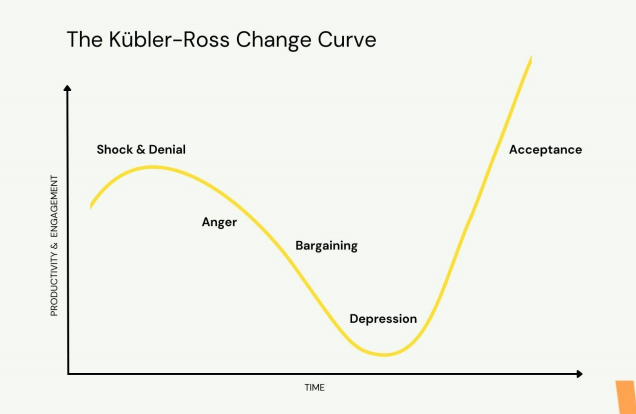
\includegraphics[width=0.5\linewidth]{figures/Week 7/KR Curve.png}
\end{figure}

\bigskip

\noindent\textbf{Stages of the Change curve}:

\begin{itemize}
    \item Shock and Denial
    \begin{itemize}
        \item In IT: “The old system works fine. This project will never happen.”
        \item CM Focus: Provide clear information about why the change is happening
    \end{itemize}
    \item Anger
    \begin{itemize}
        \item - In IT: “Why are we forced to use this? Management doesn’t understand our work!”
        \item CM Focus: Encourage listening and empathy; give people a safe channel to voice concerns
    \end{itemize}
    \item Bargaining
    \begin{itemize}
        \item In IT: “Can’t we keep using the old CRM for some tasks? Maybe run both in parallel?”
        \item CM Focus: Provide clarity on non-negotiables and offer small flexibilities where possible.
    \end{itemize}
    \item Depression
    \begin{itemize}
        \item In IT: “This is too hard. Productivity is dropping. I can’t keep up.”
        \item CM Focus: Offer training, coaching, and peer support. Share quick wins to rebuild confidence.
    \end{itemize}
    \item Acceptance
    \begin{itemize}
        \item In IT: “Okay, I can see the benefits now. This system actually makes my job easier.”
        \item CM Focus: Reinforce positive behaviours, celebrate successes, embed the change into culture.
    \end{itemize}
\end{itemize}

\subsubsection{Key implications for IT Projects}

\indent 

Transition state is the riskiest $\xrightarrow{}$ confusion, mistakes, drop in productivity.

Change managers need to provide communication, training, and support to help people move through the curve.

Success depends on moving the majority from resistance to commitment efficiently.

\subsubsection{Psychology of Change}

\noindent Why does psychology matter in IT Change?

Even the best-designed IT systems fail \textbf{if people resist} or refuse to adopt them.

Change creates \textbf{uncertainty} $\xrightarrow{}$ humans are wired to seek stability, routine, and control.

Psychology helps us understand \textbf{why people resist} and \textbf{how to support them}.

\bigskip

\noindent \textbf{Common Psychological Responses}

\begin{itemize}
    \item \textbf{Fear of the Unknown}: “What will this mean for my job?”
    \item \textbf{Loss Aversion}: People value what they already have more than what they might gain.
    \item \textbf{Cognitive Dissonance}: Conflict between old habits and new expectations.
    \item \textbf{Status Quo Bias}: Preference to “keep things as they are.”
    \item \textbf{Social Proof}: People adopt changes faster when they see peers/colleagues doing so.
\end{itemize}

\bigskip

\noindent\textbf{Theories and perspectives}

\begin{itemize}
    \item Change agents must be conscious of both a sender's mentality and the receiver's orientation.
    \item Employee resistance is the norm, not the exception. Expect some to never support the change.
    \item Visible and active sponsorship is not only desirable but necessary for success.
    \item Value systems have a direct impact on how employees react to change.
    \item The size of change determines how much and what kind of change management is needed.
    \item The "right" answer is not enough to successfully implement change.
    \item Employees go through the change process in stages and go through these stages as individuals.
\end{itemize}

\noindent\textbf{Supporting Psychology of Change}:

\begin{itemize}
    \item \textbf{Empathy}: listen and acknowledge concerns.
    \item \textbf{Communication}: explain the “why,” not just the “what.”
    \item \textbf{Involvement}: give people a voice in shaping the change.
    \item \textbf{Training \& Coaching}: reduce anxiety by building competence.
    \item \textbf{Reinforcement \& Recognition}: reward early adopters, celebrate progress
\end{itemize}

\subsubsection{Managing Change Effectively}

\indent

Everyone has a different pace of adapting to change. This can be seen through the Diffusion of Innovation Theory:

\begin{itemize}
    \item \textbf{Early adopters}: curious, motivated by innovation.
    \item \textbf{Majority}: wait until they see proof of benefits.
    \item \textbf{Laggards}: fear loss, need strong support to shift.
\end{itemize}

\bigskip

\noindent\textbf{Core principles of Effective Change Management}

\begin{itemize}
    \item \textbf{Clarity of Purpose}: Communicate the why (business case, benefits).
    \item \textbf{Leadership Commitment}: Senior leaders must actively champion the change.
    \item \textbf{Stakeholder Engagement}: Involve the right people early, listen to concerns.
    \item \textbf{Structured Process}: Follow a proven framework (ADKAR, Kotter, etc.).
    \item \textbf{Continuous Support}: Training, coaching, feedback channels throughout the transition.
\end{itemize}

\bigskip

\noindent  Key activities in IT Projects:

\begin{itemize}
    \item Build awareness and desire: Explain why change is necessary
    \item Develop capability: Provide training, job aids, and coaching
    \item Reinforce adoption: Recognise early adopters, collect feedback, and adjust quickly
\end{itemize}

\subsubsection{Practical Strategies for IT Change}

\begin{itemize}
    \item \textbf{Communication Plan}:
    \begin{itemize}
        \item Tailored messaging for executives, managers, end-users.
        \item Multi-channel: town halls, FAQs, videos, Slack/Teams updates.
    \end{itemize}
    \item \textbf{Stakeholder Mapping \& Resistance Management}:
    \begin{itemize}
        \item Identify “high influence, low support” individuals early.
        \item Convert them into champions or neutralize risks.
    \end{itemize}
    \item \textbf{Quick Wins \& Iterative Delivery}:
    \begin{itemize}
        \item Agile-style pilots $\xrightarrow{}$ demonstrate success quickly.
        \item Use feedback loops to refine adoption strategies.
    \end{itemize}
    \item \textbf{Change Agents Network}:
    \begin{itemize}
        \item Identify respected staff in each department.
        \item Train them to support peers → peer influence accelerates adoption.
    \end{itemize}
\end{itemize}

\subsubsection{Change and Business \& IT outcomes}

\indent

\noindent Why is change and outcomes related?

\begin{itemize}
    \item IT projects succeed only when \textbf{people adopt the change}.
    \item Without adoption → business value is never realized (new system unused, shadow IT emerges, money wasted).
    \item Effective OCM ensures the investment in technology translates into results.
\end{itemize}

\bigskip 

\noindent On successful change management, a few business outcomes could be:

\begin{itemize}
    \item Higher Productivity: Faster processes, reduced errors, smoother workflows.
    \item Customer Satisfaction: Improved service delivery, quicker response times.
    \item Employee Engagement: Staff feel supported and involved → reduced turnover.
    \item Innovation Readiness: Organization builds resilience for future changes.
\end{itemize}

\bigskip On successful change management, a few IT outcomes could be:

\begin{itemize}
    \item Adoption Rates: Percentage of users actively engaging with the new system.
    \item System Utilization: Depth of features being used vs. basic functions only.
    \item Process Compliance: Are new workflows followed, or do people revert to old ways?
    \item Governance Alignment: Supports ITIL Change Enablement and compliance standards.
\end{itemize}

\subsection{OCM Models and Frameworks}

\subsubsection{McKinsey's 7s Model}

\indent 

It is a holistic framework to analyze and align an organization during change. It focuses on \textbf{seven interdependent elements}, divided into hard and soft factors.

\begin{itemize}
    \item Hard S’s (easier to identify \& manage):
    \begin{itemize}
        \item \textbf{Strategy}: the plan to build competitive advantage.
        \item \textbf{Structure}: organizational hierarchy, reporting lines.
        \item \textbf{Systems}: processes, workflows, and IT systems.
    \end{itemize}
    \item Soft S’s (harder to define, but critical for success):
    \begin{itemize}
        \item \textbf{Shared Values}: the organization’s core beliefs and culture (the central point).
        \item \textbf{Skills}: capabilities and competencies of staff.
        \item \textbf{Style}: leadership style and management approach.
        \item \textbf{Staff}: people, roles, and talent management.
    \end{itemize}
\end{itemize}

\bigskip

\noindent\textbf{Benefits of this model}

\begin{itemize}
    \item Encourages \textbf{holistic thinking} (not just focusing on systems or strategy).
    \item Identifies \textbf{misalignments} that block change (e.g., great strategy but no skills to execute).
    \item Useful for diagnosing why change is stalling.
    \item Can act as a \textbf{checklist} during IT and business transformation.
\end{itemize}

\bigskip

\noindent \textbf{When to use?}

\begin{itemize}
    \item During \textbf{major IT implementations} (ERP, HRMS, CRM, etc.) to ensure people, processes, and systems align.
    \item For \textbf{organizational restructuring}.
    \item To \textbf{assess readiness} for change.
    \item To \textbf{troubleshoot failing projects} by identifying gaps.
\end{itemize}

\subsubsection{ADKAR Model}

\indent 

Focuses on guiding \textbf{individuals through change}, step by step. The acronym stands for the \textbf{five building blocks} of successful change.

\begin{itemize}
    \item \textbf{A – Awareness}
    \begin{itemize}
        \item People understand why the change is happening.
        \item “Why this change? Why now?”
    \end{itemize}
    \item \textbf{D – Desire}
    \begin{itemize}
        \item Individuals are motivated to support the change.
        \item Overcomes resistance by showing personal and organizational benefits.
    \end{itemize}
    \item \textbf{K – Knowledge}
    \begin{itemize}
        \item Training and communication provide people with how to change.
        \item Skills, tools, and understanding are built.
    \end{itemize}
    \item \textbf{A – Ability}
    \begin{itemize}
        \item People apply knowledge and perform in the new way.
        \item Requires practice, coaching, and support.
    \end{itemize}
    \item \textbf{R – Reinforcement}
    \begin{itemize}
        \item Sustains change through recognition, rewards, and performance tracking.
        \item Prevents “slipping back” into old habits.
    \end{itemize}
\end{itemize}

\bigskip

\noindent\textbf{Benefits of the model}

\begin{itemize}
    \item \textbf{Simple, people-centered framework} (easy to teach and apply).
    \item Breaks down change into \textbf{manageable, actionable steps}.
    \item Highlights that \textbf{change happens at the individual level first}.
    \item Helps managers \textbf{diagnose resistance} (e.g., if adoption is failing, is it Awareness or Ability that’s missing?).
\end{itemize}

\bigskip

\noindent\textbf{When to use?}

\begin{itemize}
    \item IT rollouts where \textbf{end-user adoption} is key (e.g., CRM, ERP, HRMS).
    \item Agile projects requiring \textbf{continuous adoption}.
    \item Situations with \textbf{high resistance} where people need structured support.
    \item \textbf{Training and enablement programs} linked to IT change.
\end{itemize}

\subsubsection{Kotter's 8 step change model}

\indent 

A \textbf{top-down approach} to managing organizational change.

Focuses on creating momentum and embedding change into culture.

\noindent\textbf{The 8 steps}:

\step Create a sense of urgency: Show why change is needed now.

\step Build a Guiding Coalition: Form a strong team of leaders and influencers to drive change.

\step Develop a vision and strategy: Provide a clear direction for the change and how it benefits the organization.

\step Communicate the change vision: Share the message widely and consistently. Use multiple channels (emails, town halls, team meetings).

\step Empower Employees for action: Remove barriers and provide resources.

\step Generate short term wins: Show quick, visible results to keep motivation high.

\step Consolidate gains and produce more change: Use early successes to drive further change. Don’t declare victory too soon.

\step Anchor new approaches in the culture: Embed change into policies, processes, and values.

\bigskip

\noindent\textbf{Benefits of the model}:

\begin{itemize}
    \item Provides a \textbf{structured roadmap} for large-scale change.
    \item Focuses on \textbf{leadership and communication}.
    \item Ensures \textbf{momentum is sustained} beyond early wins.
    \item Particularly strong for \textbf{strategic IT transformations}.
\end{itemize}

\bigskip

\noindent\textbf{When to use?}

\begin{itemize}
    \item Large, organization-wide IT changes (e.g., digital transformation, ERP rollout).
    \item When culture change is essential for adoption.
    \item In hierarchical organizations where \textbf{leadership sponsorship} is critical.
\end{itemize}

\subsection{Questions}

\subsubsection{End of Lecture Questions}

\begin{itemize}
    \item What is the difference between project management and change management? Why do IT projects need both?
    \item How does change management contribute to business and IT outcomes? Give one business outcome and one IT outcome.
    \item Compare the McKinsey 7S, ADKAR, and Kotter’s 8-step models. In which scenarios would each be most effective?
    \item How does OCM support IT governance and frameworks such as ITIL Change Enablement?
\end{itemize}

\subsubsection{Case Study}

\indent 

Alpha Manufacturing is a mid-sized company that decides to implement a new Enterprise Resource Planning (ERP) system to integrate finance, supply chain, and HR.

The Project Management team focuses on budget, schedule, and vendor 
coordination.

The Change Management team is tasked with employee adoption and 
training.

\noindent Challenges emerging:

\begin{itemize}
    \item Many employees are skeptical, saying the old systems “work fine.”
    \item Line managers feel excluded from decision-making.
    \item Training sessions are poorly attended.
    \item A pilot rollout showed low adoption: employees continue using spreadsheets.
    \item The CIO is under pressure to show ROI within 12 months.
\end{itemize}

\bigskip

\noindent\textbf{Questions}:

\begin{itemize}
    \item At which stage(s) of the change curve do Alpha’s employees seem to be?
    \item What psychological factors might be causing resistance to the ERP system?
    \item Which change management model (McKinsey 7S, ADKAR, or Kotter’s 8-step) would you apply to this situation? Why?
    \item What 2–3 practical steps could the Change Management team take to increase adoption and reduce resistance?
\end{itemize}
\pagebreak

\section{Week 8 - Quality Assurance and Software Testing}
\subsection{Foundations of Quality in IT}

\subsubsection{Quality in IT}

\indent

\noindent\textbf{Quality in IT} refers to how well a software product or IT service meets stakeholder needs and expectations, while being reliable, secure, and maintainable.

\bigskip

\noindent Dimensions of Quality in Software:

\begin{itemize}
    \item Functionality: Does the system do what it’s supposed to do?
    \item Reliability: Can it perform consistently under expected conditions?
    \item Usability: Is it user-friendly and accessible?
    \item Efficiency: Does it use resources (CPU, memory, bandwidth) optimally?
    \item Maintainability: How easy is it to update, fix, or improve?
    \item Portability: Can it be deployed in different environments easily?
    \item Security: Can it protect data and resist threats?
\end{itemize}

\bigskip

\noindent Why does Quality matter in IT?

\begin{itemize}
    \item \textbf{Business perspective}: Enhances customer satisfaction, reduces costs of rework, builds trust.
    \item \textbf{Technical perspective}: Prevents bugs, system crashes, and vulnerabilities.
    \item \textbf{Professional/ethical perspective}: IT professionals have a responsibility to deliver safe and reliable systems.
\end{itemize}

\bigskip 

\noindent Cost of Poor Quality in IT

\begin{itemize}
    \item Direct costs: Bug fixes, downtime, data loss.
    \item Indirect costs: Reputational damage, loss of clients, potential legal issues.
\end{itemize}

\subsubsection{Quality Assurance}

\indent 

\textbf{Quality Assurance (QA)}: A \textbf{proactive}, \textbf{process-oriented approach} that ensures software and IT services meet defined standards and stakeholder expectations.

Focuses on \textbf{preventing defects} rather than just detecting them. Ensures that the \textbf{processes used to create deliverables} are effective and reliable.

\bigskip

\noindent Objectives:

\begin{itemize}
    \item Ensure that software meets requirements and complies with standards.
    \item Minimize defects by improving development and testing processes.
    \item Improve efficiency of teams through standardized workflows.
    \item Build customer confidence and trust in IT systems.
\end{itemize}

\subsubsection{Quality Control}

\indent 

\textbf{Quality Control (QC)}: A reactive, product-oriented process that ensures deliverables meet defined quality standards.

Focuses on \textbf{detecting defects} in the product or service after development has begun. Ensures the output matches requirements and specifications.

\bigskip

\noindent Objectives:

\begin{itemize}
    \item Verify that the final product is reliable and fit for purpose.
    \item Detect and document defects or deviations from requirements.
    \item Ensure compliance with customer and regulatory standards.
    \item Provide feedback for process improvement (links back to QA).
\end{itemize}

\subsubsection{Testing}

\indent 

\textbf{Software Testing}: The process of \textbf{executing a system or application} with the intent of finding defects and verifying it meets specified requirements.

A \textbf{subset of Quality Control (QC)}.

Focused on \textbf{validation} (Are we building the right product?) and \textbf{verification} (Are we building the product right?).

\bigskip

Main purpose of testing:

\begin{itemize}
    \item To find defects before the software reaches users.
    \item To ensure the product meets functional and non-functional requirements.
    \item To reduce risks (financial, safety, reputational).
    \item To increase confidence in the product.
\end{itemize}

\subsection{Quality Assurance in IT}

\indent 

\noindent\textbf{Quality Assurance (QA) in IT}: A systematic process to ensure that IT systems, software, and services \textbf{consistently meet requirements}, \textbf{industry standards}, and \textbf{user expectations}.

\bigskip

It goes beyond software, it covers: \textbf{Infrastructure} (servers, networks, cloud), \textbf{Processes} (SDLC, ITIL practices), \textbf{Information Security} (compliance, audits).

\subsubsection{QA standards}

\indent 

\noindent\textbf{Quality Standards}: Agreed-upon criteria, guidelines, or frameworks used to \textbf{ensure IT systems, software, and processes meet quality requirements}.

\bigskip

They provide \textbf{consistency, reliability, and assurance} across projects, teams, and organizations.

Standards are often \textbf{internationally recognized} (ISO, IEEE) or \textbf{industry specific}.

Quality standards are important as:

\begin{itemize}
    \item Ensures processes are repeatable and auditable.
    \item Provides benchmarks for performance, security, and reliability.
    \item Supports compliance with laws and regulations.
    \item Reduces risk of failures and costly defects.
    \item Facilitates continuous improvement and professional accountability.
\end{itemize}

\subsubsection{ISO 9000}

\indent

\textbf{ISO 9000} is a family of international standards developed by the \textbf{International Organization for Standardization (ISO)}.

Goal: Ensure organizations consistently deliver \textbf{products} and \textbf{services} that \textbf{meet customer and regulatory requirements}.

\bigskip

\noindent Main principles:

\begin{itemize}
    \item Customer focus: Meeting or exceeding customer expectations.
    \item Leadership: Establishing unity of purpose and direction.
    \item Engagement of people: Involving staff at all levels.
    \item Process approach: Managing activities as processes for efficiency.
    \item Improvement: Continuous organizational learning and enhancement.
    \item Evidence-based decision making: Using data and facts for decisions.
    \item Relationship management: Managing relationships with stakeholders (suppliers, partners, regulators).
\end{itemize}

\bigskip

\noindent Why is ISO-9000 important in IT?

IT projects often involve complex processes, multiple stakeholders, and high risks.

ISO 9000 ensures:

\begin{itemize}
    \item Clear processes for software development, testing, and delivery.
    \item Consistency across multiple projects and teams.
    \item Customer trust in reliable and repeatable outcomes.
    \item Continuous improvement in IT service delivery
\end{itemize}

\bigskip

\noindent Benefits of ISO-9000

\begin{itemize}
    \item Standardized documentation and reporting.
    \item Better process control and efficiency.
    \item Fewer defects and failures.
\end{itemize}

\subsubsection{ISO 27001}

\indent

\textbf{ISO/IEC 27001} is an international standard for \textbf{Information Security Management Systems (ISMS)}.

Published by the \textbf{International Organization for Standardization (ISO)} and the \textbf{International Electrotechnical Commission (IEC)}.

Provides a \textbf{systematic approach} to managing sensitive company and customer information so it remains \textbf{confidential, accurate, and available}.

\bigskip

\noindent The main objectives of ISO27001 are:

\begin{itemize}
    \item Protect confidentiality, integrity, and availability (CIA triad) of information.
    \item Establish an ISMS: a structured framework of policies, processes, and controls.
    \item Reduce risks such as data breaches, hacking, insider threats, or human errors.
    \item Provide compliance with legal, regulatory, and contractual requirements.
\end{itemize}

\bigskip

\noindent The key components of ISO 27001 are:

\begin{itemize}
    \item \textbf{Risk Assessment}: Identify and evaluate information security risks.
    \item \textbf{Security Controls}: 114 controls grouped into 14 categories
    \item \textbf{Continuous Improvement}: Regularly monitor, review, and improve the ISMS.
    \item \textbf{Management Involvement}: Top management commitment is essential.
\end{itemize}

\bigskip

ISO 27001 is important in IT as:

\begin{itemize}
    \item IT systems handle sensitive data: customer records, financial data, intellectual property and Cyber threats are increasingly sophisticated.
    \item ISO 27001 helps organisations:
    \begin{itemize}
        \item Demonstrate trustworthiness to clients.
        \item Reduce the likelihood and impact of breaches.
        \item Align with other compliance requirements (e.g., GDPR, HIPAA, APRA in Australia).
    \end{itemize}
\end{itemize}

\subsubsection{Quality Assurance and Governance Frameworks}

\indent 

A \textbf{governance framework} defines the structures, processes, and practices that ensure IT activities are aligned with \textbf{business objectives}, \textbf{regulations}, and \textbf{quality standards}.

\bigskip 

In QA, governance ensures that:

\begin{itemize}
    \item Quality processes are not ad-hoc but institutionalized.
    \item Roles and responsibilities are clearly defined.
    \item Compliance with standards (ISO, CMMI, IEEE, ITIL, etc.) is monitored.
\end{itemize}

\bigskip

\textbf{QA} ensures that products and processes meet agreed quality standards.

Governance provides the \textbf{oversight and accountability} to ensure QA is applied consistently across projects.

Together, they create a \textbf{culture of quality and accountability} in IT organizations.

\subsubsection{Key QA and Governance Frameworks}

\indent 

\begin{itemize}
    \item ITIL
    \begin{itemize}
        \item Focus: IT Service Management (ITSM).
        \item QA Role: Provides processes for incident, change, and problem management, ensuring consistent service delivery.
    \end{itemize}
    \item COBIT
    \begin{itemize}
        \item Focus: IT governance and management.
        \item QA Role: Emphasizes control, risk management, and process maturity.
    \end{itemize}
    \item CMMI
    \begin{itemize}
        \item Focus: Process maturity in software and systems engineering.
        \item QA Role: Provides a structured roadmap to process improvement across maturity levels.
    \end{itemize}
\end{itemize}

\subsubsection{The Deming Cycle}

\indent 

Also known as the \textbf{PDCA Cycle}: Plan $\xrightarrow{}$ Do $\xrightarrow{}$ Check $\xrightarrow{}$ Act.

A continuous improvement model used in quality assurance, process management, and governance frameworks.

This 4 stages are:

\begin{itemize}
    \item \textbf{Plan}: Identify problems or opportunities.
    \item \textbf{Do}: Implement the plan on a small scale.
    \item \textbf{Check}: Monitor and evaluate results against expected outcomes.
    \item \textbf{Act}: Standardize successful practices.
\end{itemize}

\subsubsection{Capability Maturity Model Integration (CMMI)}

\begin{figure}[h]
    \centering
    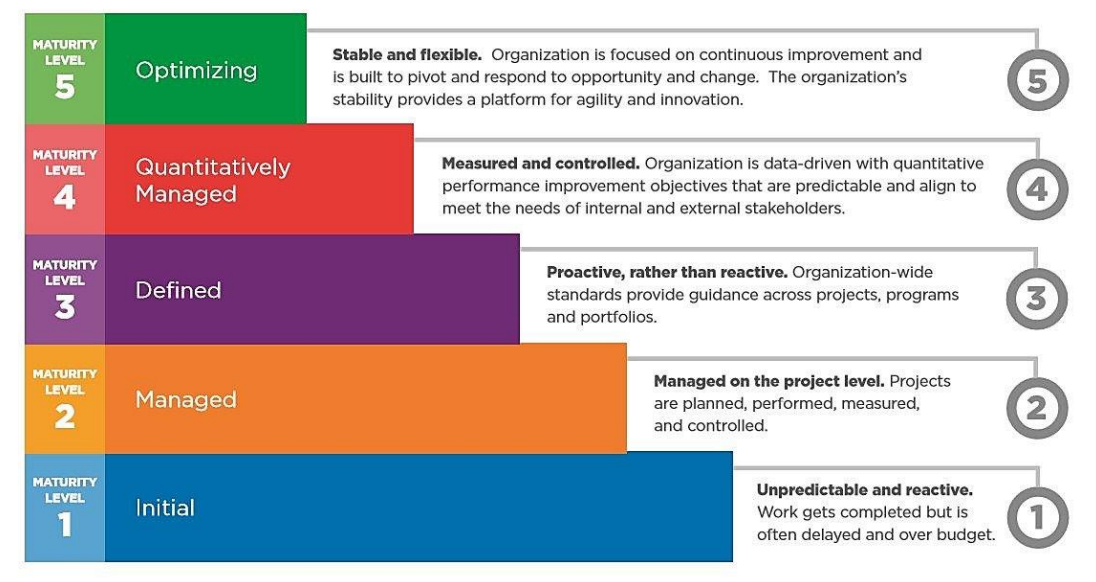
\includegraphics[width=0.9\linewidth]{figures/Week 8/CMMI.png}
\end{figure}

A \textbf{process improvement framework} that helps organizations \textbf{develop}, \textbf{refine}, and \textbf{measure maturity in processes} for software, systems, and service delivery.

Used in IT, engineering, defense, healthcare, and finance industries.

CMMI integrates closely with QA because QA ensures \textbf{processes are followed consistently}, CMMI ensures those processes are \textbf{mature, measurable, and improving}.

Often combined with \textbf{ISO 9001} and the \textbf{Deming Cycle} for continuous process improvement.

\subsubsection{The Deming cycle and CMMI Maturity Levels}

\indent 

\begin{figure}
    \centering
    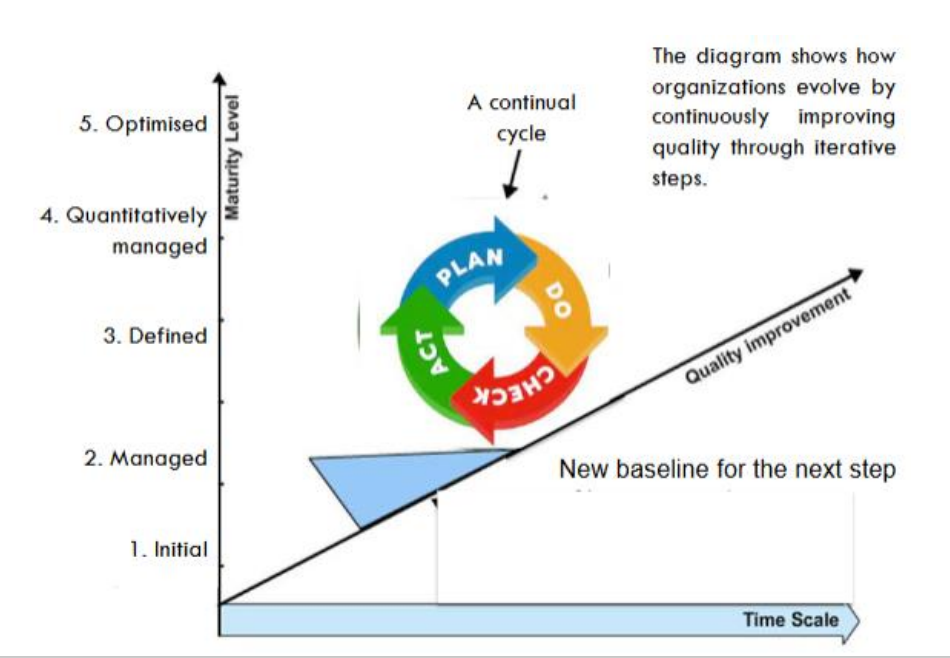
\includegraphics[width=0.8\linewidth]{figures/Week 8/Deming CMMI.png}
\end{figure}

The Deming Cycle (PDCA: Plan–Do–Check–Act) provides a foundation for \textbf{continuous improvement}.

CMMI (Capability Maturity Model Integration) provides a \textbf{structured maturity roadmap} for organizations to evolve their processes.

Together:

\begin{itemize}
    \item Deming $\xrightarrow{}$ How to improve continuously.
    \item CMMI $\xrightarrow{}$ Where the organization stands on process maturity and what the next step is.
\end{itemize}

\bigskip

CMMI Maturity levels:

\begin{itemize}
    \item \textbf{Level 1}: Processes are ad hoc, chaotic. No PDCA cycle in place.
    \item \textbf{Level 2}: Basic planning (Plan) and execution (Do) exist at the project level. However, limited measurement (Check) and corrective actions (Act).
    \item \textbf{Level 3}: Processes are standardized and documented across the organization and consistent Plan–Do; some Check–Act to refine processes.
    \item \textbf{Level 4}: Check phase is emphasized → processes are measured and controlled statistically. Decisions are data-driven.
    \item \textbf{Level 5}: Continuous Act phase → proactive improvements and innovations.
\end{itemize}

\subsubsection{Quality Audits}

\indent 

A Quality Audit is a systematic, independent examination to determine whether activities and related results comply with planned arrangements (such as standards, processes, and requirements) and whether these arrangements are effectively implemented and suitable to achieve objectives.

\bigskip

Main objectives:

\begin{itemize}
    \item Verify compliance with standards, processes, and guidelines.
    \item Identify gaps, inefficiencies, or risks in quality practices.
    \item Recommend improvements for continuous quality enhancement.
    \item Build organizational trust and credibility.
\end{itemize}

\bigskip

Types of Quality Audits:

\begin{itemize}
    \item \textbf{Internal Audits (First-party)}: Conducted by the organization itself. Helps ensure compliance with internal standards and identify early issues.
    \item \textbf{External Audits (Second- and Third-party)}: Conducted by external clients, certification bodies, or regulatory agencies. Ensures independent validation of compliance (e.g., ISO 9000 certification audits).
    \item \textbf{Process Audits}: Focus on whether processes are being followed correctly.
    \item \textbf{Product Audits}: Verify that the end product meets quality specifications and requirements.
    \item \textbf{System Audits}: Evaluate the organization’s overall quality management system (QMS)
\end{itemize}

\subsection{Software Testing Fundamentals}

\subsubsection{Software Testing Lifecycle}

\indent 

\noindent\textbf{Software Testing Lifecycle}: A sequence of specific activities conducted during the testing process to ensure that software meets quality standards.

\bigskip  

Just like the Software Development Lifecycle (SDLC), the STLC is a framework, but it focuses exclusively on \textbf{verification and validation of software}.

\bigskip

\noindent Key features:

\begin{itemize}
    \item Parallel activity to SDLC: Testing starts as soon as requirements are available (shift-left testing).
    \item Iterative process: May repeat for each sprint, release, or version.
    \item Ensures quality at every stage, not just at the end.
\end{itemize}

\subsubsection{Testing Phases}

\begin{table}[h]
\centering
\begin{tabular}{|c|l|l}
\cline{1-2}
\textbf{Phase}                                                                   & \multicolumn{1}{c|}{\textbf{Description}}                                                                                                                                                                  &  \\ \cline{1-2}
\textbf{Requirements}                                                            & \begin{tabular}[c]{@{}l@{}}QA team analyzes requirements (functional and non-functional). \\ They will identify testable requirements and involve stakeholders\\  to clarify any ambiguities.\end{tabular} &  \\ \cline{1-2}
\textbf{Planning}                                                                & \begin{tabular}[c]{@{}l@{}}Define scope, objectives, resources, schedule, and responsibilities. \\ Risks are assessed and mitigation strategies developed.\end{tabular}                                    &  \\ \cline{1-2}
\textbf{Development}                                                             & \begin{tabular}[c]{@{}l@{}}Design test cases with detailed input, expected output, and conditions. \\ Create test data and perform peer review of test cases.\end{tabular}                                 &  \\ \cline{1-2}
\textbf{\begin{tabular}[c]{@{}c@{}}Environment\\ setup\end{tabular}}             & \begin{tabular}[c]{@{}l@{}}Prepare hardware, software, network, and tools for testing. \\ Often involves DevOps pipelines or containerized environments \\ (Docker, Kubernetes, etc.).\end{tabular}        &  \\ \cline{1-2}
\textbf{Execution}                                                               & \begin{tabular}[c]{@{}l@{}}Execute test cases manually or using automation and \\ log test results to raise defect/bug reports for failures.\end{tabular}                                                  &  \\ \cline{1-2}
\textbf{\begin{tabular}[c]{@{}c@{}}Defect reporting\\ and tracking\end{tabular}} & \begin{tabular}[c]{@{}l@{}}Log defects in a bug-tracking system. Prioritise defects \\ and work with developers to ensure timely resolution.\end{tabular}                                                  &  \\ \cline{1-2}
\textbf{Test cycle closure}                                                      & \begin{tabular}[c]{@{}l@{}}Evaluate exit criteria \\ (e.g., all planned test cases executed, critical defects closed). \\ Analyse test coverage and prepare a test summary report (TSR).\end{tabular}      &  \\ \cline{1-2}
\end{tabular}
\end{table}

\subsubsection{Test Artifacts}

\indent 

\textbf{Test artifacts} are the \textbf{documents, deliverables, and by-products} produced during the Software Testing Lifecycle (STLC).

They provide evidence of testing activities, support traceability, and help stakeholders assess software quality.

They can be created before, during, or after testing, and serve as a reference for both current and future projects.

\bigskip

\noindent Benefits of test artifacts:

\begin{itemize}
    \item Traceability: Connects requirements to tests to ensure nothing is missed.
    \item Accountability: Provides evidence of due diligence and compliance (e.g., ISO, CMMI).
    \item Communication: Helps stakeholders (managers, clients, auditors) understand quality status.
\end{itemize}

\subsubsection{Important Test artifacts}

\indent 

\textbf{Test Plan} is a high-level document that defines the scope, approach, objectives, resources, schedule, and responsibilities of testing activities.

Key components:

\begin{itemize}
    \item Objectives and scope of testing
    \item Features to be tested / not tested
    \item Test environment setup
    \item Roles and responsibilities
    \item Schedule and milestones
    \item Risks and mitigation strategies
    \item Tools to be used
\end{itemize}

\bigskip  

A \textbf{Test Case} is a detailed, step-by-step set of instructions to validate a particular functionality of the software. It describes input, execution conditions, and expected output.

Key elements:

\begin{itemize}
    \item Test Case ID
    \item Preconditions (setup required)
    \item Test Steps (actions to perform)
    \item Expected Result
    \item Actual Result (during execution)
    \item Status (Pass/Fail)
\end{itemize}

\bigskip

\textbf{Test Data} refers to the \textbf{input values} (valid, invalid, boundary cases) used in test cases to verify expected system behavior. It ensures tests are realistic and cover a wide range of scenarios.

Types of test data:

\begin{itemize}
    \item Valid Data: Correct input values (e.g., correct username \& password).
    \item Invalid Data: Incorrect inputs (e.g., wrong password, empty fields).
    \item Boundary Data: Edge cases (e.g., password length exactly 8 or 20 chars).
    \item Large Volume Data: For performance/load testing.
\end{itemize}

\newpage

\subsection{Types of Testing}

\subsubsection{Functional vs Non-functional Testing}

\begin{table}[h]
\centering
\begin{tabular}{|c|l|l|}
\hline
\textbf{Aspect}                                                           & \multicolumn{1}{c|}{\textbf{Functional Testing}}                                                                                 & \multicolumn{1}{c|}{\textbf{Non-functional Testing}}                                                                                 \\ \hline
\textbf{Purpose}                                                          & \begin{tabular}[c]{@{}l@{}}Verify that the system\\ behaves according to specified\\ requirements or functionality.\end{tabular} & \begin{tabular}[c]{@{}l@{}}Evaluate how well the system\\ performs under specific conditions\\ (quality attributes).\end{tabular}    \\ \hline
\textbf{Focus}                                                            & \textit{\begin{tabular}[c]{@{}l@{}}What the system does\\ (features, operations,\\ user interactions).\end{tabular}}             & \textit{\begin{tabular}[c]{@{}l@{}}How the system behaves\\ (performance, usability,\\ reliability, security).\end{tabular}}         \\ \hline
\textbf{\begin{tabular}[c]{@{}c@{}}Requirement\\ source\end{tabular}}     & \begin{tabular}[c]{@{}l@{}}Functional requirements\\ (e.g., “User can log in with\\ a username/password”).\end{tabular}          & \begin{tabular}[c]{@{}l@{}}Non-functional requirements\\ (e.g., “System must handle\\ 1000 concurrent users”).\end{tabular}          \\ \hline
\textbf{Test data}                                                        & \begin{tabular}[c]{@{}l@{}}Typically deterministic\\ input/output scenarios.\end{tabular}                                        & \begin{tabular}[c]{@{}l@{}}Often metrics-based:\\ response times, throughput,\\ error rates.\end{tabular}                            \\ \hline
\textbf{\begin{tabular}[c]{@{}c@{}}Automation\\ feasibility\end{tabular}} & \begin{tabular}[c]{@{}l@{}}High\\ (unit and integration tests\\ are commonly automated).\end{tabular}                            & \begin{tabular}[c]{@{}l@{}}Partial\\ (some performance/security\\ tests can be automated;\\ usability is often manual).\end{tabular} \\ \hline
\textbf{\begin{tabular}[c]{@{}c@{}}Examples of\\ tests\end{tabular}}      & \begin{tabular}[c]{@{}l@{}}Unit testing,\\ Integration testing, \\ System testing,\\ User Acceptance Testing, etc.\end{tabular}  & \begin{tabular}[c]{@{}l@{}}Performance testing,\\ Security testing,\\ Usability testing,\\ Compatibility testing, etc.\end{tabular}  \\ \hline
\end{tabular}
\end{table}

\subsubsection{Functional testing - Unit Testing}

\indent 

\begin{figure}[h]
    \centering
    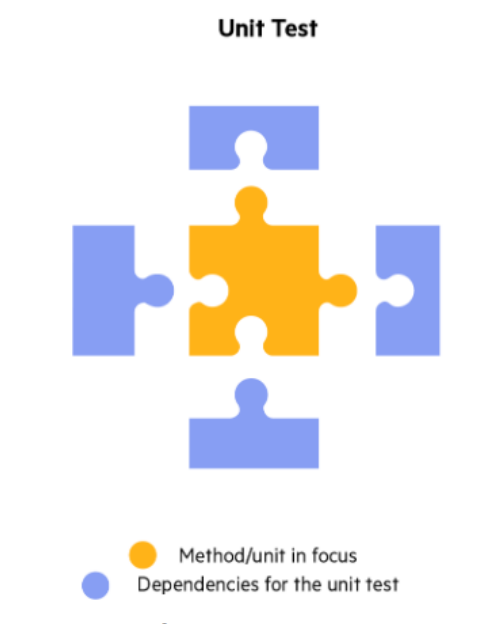
\includegraphics[width=0.3\linewidth]{figures/Week 8/Unit Testing.png}
    \caption{Unit Testing}
\end{figure}

\noindent\textbf{Unit Testing}: Testing the smallest part of an application (a function, method, or class) in isolation.

\noindent\textbf{Goal}: Ensure each unit of code works as expected.

\noindent\textbf{Who does it}: Usually developers.

\subsubsection{Functional testing - Integration Testing}

\indent 

\begin{figure}[h]
    \centering
    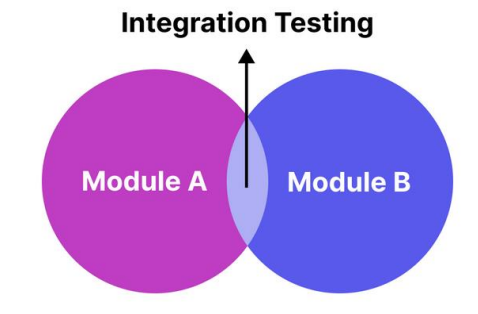
\includegraphics[width=0.5\linewidth]{figures/Week 8/Integration Testing.png}
    \caption{Integration Testing}
\end{figure}

\noindent\textbf{Integration Testing}: Testing interactions between different modules/components.

\noindent\textbf{Goal}: Verify that combined parts work together correctly.

\noindent\textbf{Approaches}:

\begin{itemize}
    \item Big Bang: test everything together at once.
    \item Top-Down: start with higher-level modules, use stubs for lower ones.
    \item Bottom-Up: start with lower modules, use drivers for higher ones.
\end{itemize}

\subsubsection{Functional testing - System Testing}

\indent 

\begin{figure}
    \centering
    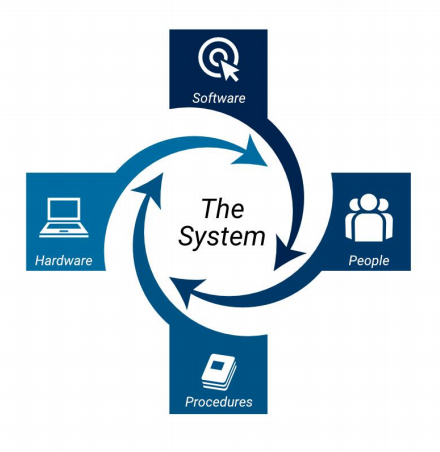
\includegraphics[width=0.3\linewidth]{figures/Week 8/System Testing.png}
    \caption{System Testing}
\end{figure}

\noindent\textbf{System Testing}Testing the complete, integrated system as a whole.
\noindent\textbf{Goal}: Validate that the software meets specified requirements.
\noindent\textbf{Conducted by}: Independent QA/test teams.

\subsubsection{Functional testing - User Acceptance Testing}

\indent 

\noindent\textbf{User Acceptance Testing}: Testing by actual users or clients before release.

\noindent\textbf{Goal}: Ensure the system meets business needs and is ready for production.

\noindent\textbf{Types}:

\begin{itemize}
    \item Alpha Testing: in-house, internal team tests with end-user perspective.
    \item Beta Testing: external users test in real-world environments.
\end{itemize}

\subsubsection{Functional testing - Black Box Testing}

\indent 

\begin{figure}[h]
    \centering
    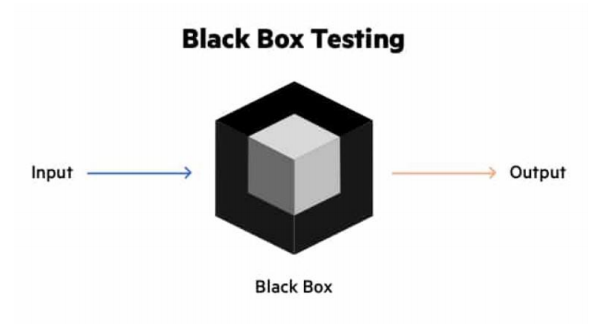
\includegraphics[width=0.3\linewidth]{figures/Week 8/Black Box.png}
    \caption{Black Box Testing}
\end{figure}

\noindent\textbf{Black Box Testing}: Testing without looking at the internal code.

\noindent\textbf{Focus}: Inputs and outputs (functionality).

\noindent\textbf{Techniques}: Boundary value analysis, equivalence partitioning.

\noindent\textbf{Example}: Entering different usernames/passwords to test login functionality

\subsubsection{Functional testing - White Box Testing}

\indent 

\begin{figure}
    \centering
    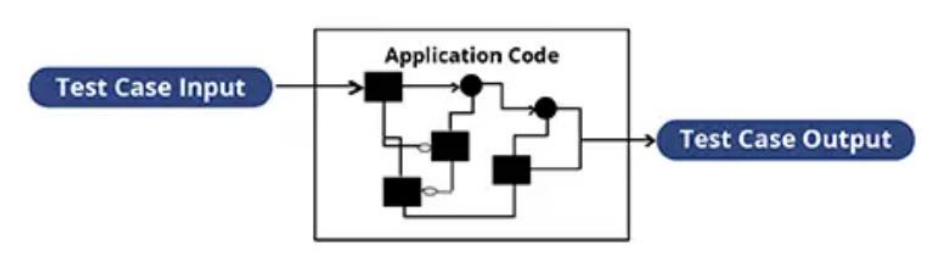
\includegraphics[width=0.3\linewidth]{figures/Week 8/White Box.png}
    \caption{White Box Testing}
\end{figure}

\noindent\textbf{White Box Testing}: Testing the internal logic, paths, and code structure.

\noindent\textbf{Focus}: Code coverage, loops, conditions.

\noindent\textbf{Who does it}: Developers/testers with coding knowledge.

\noindent\textbf{Example}: Writing tests to ensure all branches of an if-else condition execute correctly.

\subsubsection{Non-functional testing - Load Testing}

\indent 

\noindent\textbf{Load Testing}: Checking how the system performs under expected user loads.

\noindent\textbf{Goal}: Measure response time, throughput, and resource usage.

\noindent\textbf{Example}: Simulating 10,000 users logging in to a website simultaneously

\subsubsection{Non-functional testing - Stress Testing}

\indent 

\noindent\textbf{Stress Testing}: Pushing the system beyond normal limits to test breaking points.

\noindent\textbf{Goal}: Identify system stability and recovery after failure.

\noindent\textbf{Example}: Forcing a server to handle 5× expected traffic until it crashes, and observing recovery.

\subsubsection{Non-functional testing - Smoke Testing}

\indent 

\begin{figure}[h]
    \centering
    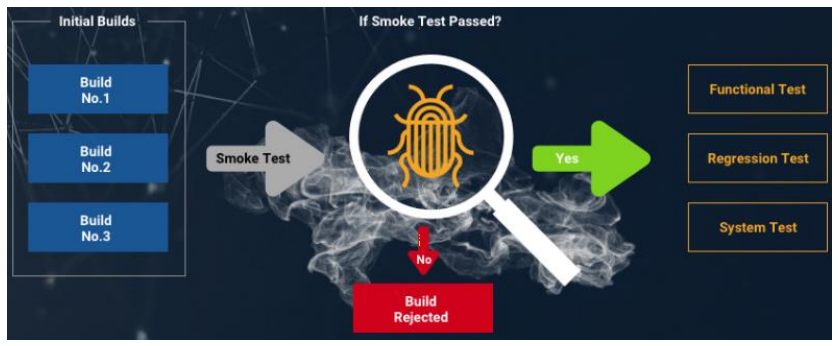
\includegraphics[width=0.8\linewidth]{figures/Week 8/Smoke Testing.png}
    \caption{Smoke Testing}
\end{figure}

\noindent\textbf{Smoke Testing}: A quick check of the basic functionality after a new build or deployment.

\noindent\textbf{Goal}: Ensure the build is stable enough for further testing (“build verification”).

\noindent\textbf{Example}: Verifying that login, navigation, and checkout buttons work after a new release.

\subsubsection{Non-functional testing - A/B Testing}

\indent 

\begin{figure}[h]
    \centering
    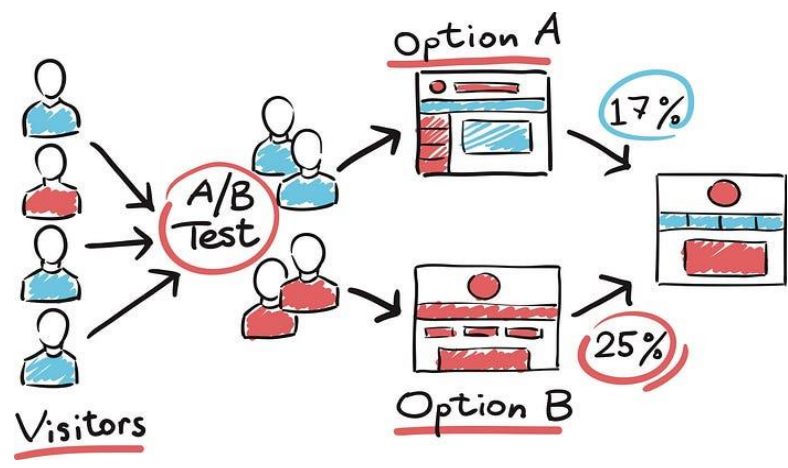
\includegraphics[width=0.8\linewidth]{figures/Week 8/A:B Testing.png}
    \caption{A:B Testing}
\end{figure}

\noindent\textbf{A:B Testing}: Comparing two versions (A and B) to see which performs better with users.

\noindent\textbf{Goal}: Improve usability, conversion, or engagement.

\noindent\textbf{Example}: Version A of a website has a red button, Version B has a blue button $\xrightarrow{}$ measure which drives more clicks.

\subsection{QA in Software Development Methodologies}

\subsubsection{QA in Waterfall}

\indent

QA in Waterfall focuses on \textbf{verification and validation} at \textbf{specific points} in the development lifecycle.

QA activities in each Waterfall Phase

\begin{itemize}
    \item \textbf{Requirements phase}: QA ensures requirements are complete, consistent, and testable.
    \item \textbf{Design phase}: QA verifies system architecture and design documents.
    \item \textbf{Implementation phase}: QA ensures coding standards are followed.
    \item \textbf{Testing phase}: Dedicated QA team executes functional and non-functional testing.
    \item \textbf{Deployment and maintenance phase}: QA ensures release readiness
\end{itemize}

\subsubsection{QA in Agile}

\indent 

QA in Agile is \textbf{integrated throughout the development lifecycle}, not just a separate phase at the end.

QA Activities in Agile:

\begin{itemize}
    \item \textbf{Continuous Requirement Analysis}: QA participates in story refinement and estimation to ensure testable and clear acceptance criteria.
    \item \textbf{Test planning in sprints}: QA plans testing for each sprint (iteration), not for the entire project upfront.
    \item \textbf{Test case design and test data}: QA collaborates closely with developers on test-driven development (TDD) and behavior-driven development (BDD).
    \item \textbf{Continuous testing}: Testing occurs throughout the sprint and defects are identified and fixed immediately, reducing rework costs.
    \item \textbf{Test automation}: Strong emphasis on automation to support fast iteration cycles.
    \item \textbf{Sprint review and retrospective}: QA participates in sprint review to validate delivered features against acceptance criteria.
\end{itemize}

\subsubsection{QA in DevOps}

\indent

QA in DevOps is fully integrated into the software delivery pipeline, emphasizing automation, monitoring, and continuous feedback.

QA activities in DevOps:

\begin{itemize}
    \item QA is \textbf{embedded in CI/CD pipelines}. This allows for early defect detection reduces risks and rework.
    \item DevOps relies heavily on \textbf{test automation} to support rapid releases.
    \item QA begins \textbf{as early as possible} in the development process.
    \item QA monitors \textbf{production environments} for errors, performance issues, and user experience.
    \item QA in DevOps is \textbf{collaborative}, involving developers, testers, operations, and security teams.
\end{itemize}

\subsubsection{Professional Issues in QA}

\indent 

Quality Assurance is not just about processes and testing, it also involves professional and ethical responsibilities. 

Professionals in QA must be aware of \textbf{issues affecting integrity}, \textbf{compliance}, and \textbf{trust} in software systems.

Ethical Responsibilities: QA professionals ensure software is safe, reliable, and meets user requirements.

Compliance and Legal issues: QA professionals must ensure software complies with regulatory and legal standards.

Confidentiality and Data privacy: QA often works with sensitive data (e.g., customer information, financial records).

\subsubsection{Future of QA and Testing}

\indent 

QA is evolving from a \textbf{phase-driven, reactive process to continuous, proactive}, and \textbf{automated quality management}.

Emerging technologies like \textbf{AI, cloud, IoT}, and \textbf{DevOps} are transforming testing practices.

Future QA professionals will need \textbf{technical, analytical}, and \textbf{collaborative skills} to ensure software quality in \textbf{complex, high-speed development environments}.

\subsubsection{How QA Roles Differ Across IT Work Environments}

\begin{table}[h]
\centering
\begin{tabular}{|c|l|l|l|}
\hline
\textbf{Aspect}                                                                 & \multicolumn{1}{c|}{\textbf{Waterfall}}                                                                       & \multicolumn{1}{c|}{\textbf{Agile}}                                                                       & \multicolumn{1}{c|}{\textbf{DevOps}}                                                                                \\ \hline
\textbf{\begin{tabular}[c]{@{}c@{}}When QA\\ happens\end{tabular}}              & At the end of the lifecycle                                                                                   & \begin{tabular}[c]{@{}l@{}}Continuous within\\ sprints\end{tabular}                                       & \begin{tabular}[c]{@{}l@{}}Built into the\\ CI/CD pipeline\end{tabular}                                             \\ \hline
\textbf{\begin{tabular}[c]{@{}c@{}}Your role as \\ a professional\end{tabular}} & \begin{tabular}[c]{@{}l@{}}QA specialist verifies \\ deliverables; strong \\ documentation focus\end{tabular} & \begin{tabular}[c]{@{}l@{}}Developers + QA \\ collaborate closely \\ shared accountability\end{tabular}   & \begin{tabular}[c]{@{}l@{}}Everyone (Dev, QA, \\ Ops, Security) \\ shares responsibility\\ for quality\end{tabular} \\ \hline
\textbf{\begin{tabular}[c]{@{}c@{}}Professional\\ Risk\end{tabular}}            & \begin{tabular}[c]{@{}l@{}}Late defect discovery \\ → high rework cost\end{tabular}                           & \begin{tabular}[c]{@{}l@{}}Missing tests in \\ fast iterations →\\ quality risk\end{tabular}              & \begin{tabular}[c]{@{}l@{}}Over-reliance \\ on automation →\\ oversight risk\end{tabular}                           \\ \hline
\textbf{\begin{tabular}[c]{@{}c@{}}Ethics and\\ Standards\end{tabular}}         & \begin{tabular}[c]{@{}l@{}}Compliance with ISO, \\ CMMI, audit checks\end{tabular}                            & \begin{tabular}[c]{@{}l@{}}Transparency with \\ stakeholders, acceptance \\ criteria clarity\end{tabular} & \begin{tabular}[c]{@{}l@{}}Continuous monitoring,\\ privacy \& security \\ compliance\end{tabular}                  \\ \hline
\end{tabular}
\end{table}

\subsection{Question}

\subsubsection{End of Lecture Questions}

\begin{itemize}
    \item Describe the Deming Cycle (PDCA) and its relevance to QA.
    \item What is CMMI, and how do its maturity levels relate to QA processes?
    \item List and briefly explain the stages of the Software Testing Lifecycle (STLC).
    \item Compare unit testing, integration testing, system testing, and UAT in terms of focus, responsibility, and timing.
    \item Explain how QA differs in Waterfall, Agile, and DevOps methodologies.
    \item How do ISO 9000 and ISO 27001 standards influence QA practices?
\end{itemize}

\subsubsection{Case Study}

\indent 

A bank is developing a new online banking platform that allows customers to log in, transfer funds, pay bills, and view transaction history. During development, several issues were observed:

\begin{itemize}
    \item A critical bug caused login failures for some users.
    \item Transaction processing slowed during peak hours.
    \item Security scans flagged a vulnerability in password storage.
    \item QA documentation was incomplete, leading to missed test cases.
\end{itemize}

\bigskip

\noindent\textbf{Questions}

\begin{itemize}
    \item Describe how traceability between requirements and test cases could prevent missed test cases.
    \item Which type of performance testing would identify the slowdown during peak hours? Explain the difference between load, stress, and soak testing in this context.
    \item Identify professional or ethical issues if the bank released the system with the known login and security issues.
    \item Considering DevOps practices, describe how continuous testing and monitoring could prevent similar issues in production.
\end{itemize}
\pagebreak

\section{Week 9 - Security Management Part 1}
\subsection{Introduction}

\subsubsection{Security}

\indent 

\textbf{Security} is the practice of protecting information systems including hardware, software, networks, and data, from unauthorized access, misuse, disruption, or destruction.

3 dimensions of security in IT:

\begin{itemize}
    \item Physical Security: Protecting the tangible infrastructure that supports IT. Goal: prevent theft, damage, or physical tampering with assets.
    \item Digital/Information Security: Protecting data and digital systems from cyber threats. Goal: maintain confidentiality, integrity, and availability of data.
    \item Operational Security: Protecting systems through processes, people, and policies. Goal: reduce risks caused by human error, insider threats, or weak processes.
\end{itemize}

\subsubsection{Security Management}

\indent 

Security Management is the process of identifying, implementing, monitoring, and continuously improving security measures to protect an organization’s assets, both physical and digital.

It ensures that risks are managed systematically, and security aligns with business objectives, compliance requirements, and operational needs.

Main goals of Security management:

\begin{itemize}
    \item Protect Confidentiality, Integrity, and Availability (CIA).
    \item Ensure business continuity.
    \item Maintain compliance and legal obligations.
    \item Build trust with users, customers, and stakeholders.
\end{itemize}

\bigskip

\noindent \textbf{Key elements of Security Management}

\begin{itemize}
    \item Risk Assessment and Analysis: Identify threats, vulnerabilities, and potential impacts.
    \item Policy and Governance: Define security policies, standards, and compliance frameworks (ISO 27001, NIST, GDPR, etc.).
    \item Implementation of Controls
    \item Monitoring and Detection: Continuous monitoring of systems, networks, and behaviors to detect anomalies.
    \item Incident Response and Recovery: Plans and procedures for containment, eradication, recovery, and lessons learned.
    \item Continuous Improvement: Regular audits, penetration testing, red/blue team exercises, feedback loops.
\end{itemize}

\bigskip 

\noindent\textbf{Why does Security management matter in IT?}

\begin{itemize}
    \item Protection of Critical Assets: IT systems store intellectual property, customer data, financial records, and operational information. Without proper security management, these assets are at risk of theft, manipulation, or destruction.
    \item Mitigating Cyber Threats: Organizations face constant attacks: malware, phishing, ransomware, insider threats. Security management ensures proactive defenses and rapid responses.
    \item Ensuring Business Continuity: Outages or breaches can cripple operations. Strong security management minimizes downtime, enabling resilience during attacks or disasters.
    \item Legal and Regulatory Compliance: Laws like GDPR, HIPAA, and standards like ISO 27001 mandate security practices. Failure to comply leads to fines, lawsuits, and reputational harm.
    \item Safeguarding Reputation and Trust: Customers, partners, and stakeholders expect organizations to handle data responsibly. Breaches erode trust and can cause lasting brand damage.
    \item Managing Human Risk: People are often the weakest link (phishing, weak passwords, negligence). Security management addresses this with training, policies, and monitoring.
    \item Cost Avoidance: The cost of prevention is far lower than the financial and operational impact of a breach.
\end{itemize}

\subsection{Understanding Vulnerabilities}

\subsubsection{Factors contributing to Vulnerabilities}

\indent 

\begin{itemize}
    \item Human Factors: Weak passwords, password reuse. Falling for phishing/social engineering. Lack of awareness or training. Insider threats (malicious or negligent employees).
    \item Technological Factors: Unpatched software and outdated systems. Misconfigurations (firewalls, cloud storage, databases). Weak encryption or lack of encryption. Zero-day vulnerabilities in hardware/software.
    \item Organisational Factors: Lack of clear policies and governance. Poor incident response planning. Insufficient monitoring and auditing. Over-reliance on third-party vendors without proper vetting.
    \item Physical/Environmental Factors: Insecure server rooms or data centers. Theft or tampering with devices. Natural disasters (floods, fires, earthquakes). Power failures or inadequate redundancy.
    \item Process and Operational Factors: Inadequate access control (too many privileges). Poor patch/change management processes.
\end{itemize}

\subsubsection{The biggest security threat - Users}

\indent

Despite all technical protections, humans are often the weakest link in security. Even the strongest firewalls, encryption, and monitoring can be bypassed if users make mistakes or act carelessly.

\noindent\textbf{Why?}

\begin{itemize}
    \item Human error: Sending sensitive information to the wrong recipient or Misconfiguring systems or accidentally deleting data.
    \item Poor password practices: Weak passwords, password reuse across accounts. Sharing credentials with others.
    \item Phishing and Social engineering: Falling for emails, calls, or messages designed to steal credentials. Clicking malicious links or downloading infected attachments.
    \item Insider threats: Disgruntled employees intentionally misusing access.
\end{itemize}

\subsection{Cyber-Crimes}

\indent 

Cyber-crimes are criminal activities that involve the internet, computers, 
networks, or digital devices. They are actions that violate laws by targeting information systems, data, or digital communications for malicious purposes. Cyber-crimes can target individuals, organizations, or governments. They often exploit technical vulnerabilities or human weaknesses. Prevention requires a combination of technical controls, policies, and user awareness.

\subsubsection{Identity Theft and Fraud}

\indent 

Identity theft occurs when someone steals another person’s personal information (like name, Social Security/Tax ID, credit card, or login credentials) to commit fraudulent activities, such as financial theft, unauthorized transactions, or impersonation.

Preventative measures:

\begin{itemize}
    \item Use strong, unique passwords and enable multi-factor authentication (MFA).
    \item Monitor accounts for suspicious activity regularly.
    \item Be cautious with sharing personal information online or over email/phone.
    \item Shred sensitive documents before disposal.
    \item Install antivirus and anti-malware software on all devices.
\end{itemize}

 \subsubsection{Harassment and Cyber-bullying}

 \indent 

\noindent\textbf{Harassment}: Repeated, unwanted behavior intended to intimidate, threaten, or disturb an individual.

\noindent\textbf{Cyberbullying}: A form of harassment that occurs \textbf{online or through digital devices}, targeting individuals with malicious intent.

Both involve misuse of digital platforms to \textbf{cause emotional, psychological, or reputational harm}.

Preventative Measures:

\begin{itemize}
    \item Implement \textbf{acceptable use policies} and online conduct rules.
    \item Monitor platforms and enforce \textbf{reporting mechanisms}.
    \item Train users on recognizing and responding to harassment.
    \item Legal and regulatory frameworks (e.g., cyber harassment laws in Australia)
\end{itemize}

\subsubsection{Hacking and Unauthorised access}

\indent

Hacking / Unauthorized access = gaining access to systems, networks, data, or accounts without permission, or using legitimate access in an unauthorized way. It covers anything from a simple password guess to sophisticated intrusion campaigns.

Preventative measures:

\begin{itemize}
    \item Strong password policies + mandatory multi-factor authentication (MFA).
    \item Least-privilege access and role-based access control (RBAC).
    \item Regular security awareness training (phishing simulations).
    \item Vendor/third-party risk assessments.
    \item Web Application Firewall (WAF) and input validation.
    \item Encryption for data at rest and in transit.
\end{itemize}

\subsubsection{Data Breaches}

\indent

A data breach occurs when sensitive, protected, or confidential information is accessed, disclosed, or stolen without authorization. This can involve personal data (PII), financial records, trade secrets, or intellectual property.

Preventative Measures:

\begin{itemize}
    \item Encrypt data at rest and in transit
    \item Implement strong access controls (least privilege, RBAC)
    \item Regular security awareness training
    \item Patch and vulnerability management
    \item Monitor and audit systems continuously
    \item Backup critical data and test recovery plans
\end{itemize}

\subsubsection{Malware}

\indent 

\textbf{Malware} (malicious software) is any software intentionally designed to \textbf{damage, disrupt, steal, or gain unauthorized access} to computer systems, networks, or data.

Preventative measures:

\begin{itemize}
    \item Install and update antivirus/anti-malware software
    \item Keep systems and software patched and up-to-date
    \item Educate users on phishing and safe browsing practices
    \item Use firewalls and intrusion detection systems
    \item Backup critical data regularly and securely
    \item Restrict unnecessary administrative privileges
\end{itemize}

\subsubsection{Phishing and Social Engineering}

\indent

\noindent\textbf{Social Engineering}: Manipulating or deceiving people to reveal confidential information or perform actions that compromise security.

\noindent\textbf{Phishing}: A type of social engineering that uses \textbf{emails, messages, or websites} to trick users into giving sensitive data (e.g., passwords, credit cards).

The key idea is that the attackers exploit \textbf{human psychology}, not just technical vulnerabilities.

Preventative measures:

\begin{itemize}
    \item User awareness and training: teach staff to recognize suspicious emails, links, and messages.
    \item Multi-factor authentication (MFA): prevents stolen credentials from being enough to access accounts.
    \item Email and web filters: block malicious content before it reaches users.
\end{itemize}

\subsubsection{DDoS Attacks}

\indent 

A \textbf{Distributed Denial of Service (DDoS)} attack aims to \textbf{overwhelm a target (server, service, network)} with traffic or requests from many distributed sources so that legitimate users cannot access it. The goal is \textbf{disruption} rather than data theft (though DDoS is sometimes used as a smokescreen for other attacks).

Preventative measures:

\begin{itemize}
    \item \textbf{Traffic scrubbing / scrubbing centres} (third-party DDoS mitigation services).
    \item \textbf{Rate limiting} and upstream filtering with ISP cooperation.
    \item \textbf{Autoscaling with careful limits}: helps absorb spikes but can be costly and must be coupled with filtering.
    \item \textbf{Load balancers} and redundancy across regions.
    \item Centralized logging, SIEM, and real-time traffic monitoring
\end{itemize}

\subsubsection{Advanced Persistent Threats (APTs)}

\indent 

An \textbf{Advanced Persistent Threat (APT)} is a \textbf{prolonged and targeted cyberattack} in which an intruder gains unauthorized access to a network and remains undetected for an extended period. APTs usually target \textbf{high-value assets} like intellectual property, financial data, or government secrets.

\begin{itemize}
    \item Preventative measures:
    \item Continuous network monitoring, anomaly detection, endpoint detection.
    \item Close known security gaps that APTs might exploit.
    \item A detailed plan to detect, contain, and remediate intrusions.
    \item Deploying Least privilege, network segmentation, and multi-factor authentication
\end{itemize}

\subsection{Security Threats and Organisational Challenges}

\indent 

\subsubsection{Categories of Security Threats}

\indent 

Security threats are potential events or actions that can compromise the confidentiality, integrity, or availability of information or systems. They can be intentional, accidental, or natural.

There are mainly 5 categories of security threats:

\begin{itemize}
    \item Human based: Threats caused by \textbf{people}, either deliberately or unintentionally.
    \item Technical: Threats exploiting \textbf{hardware, software, or network vulnerabilities}.
    \item Physical: Threats targeting the \textbf{tangible infrastructure} that supports IT.
    \item Operational: Threats arising from \textbf{weak processes, policies, or operational failures}.
    \item External: Threats from \textbf{outside the organization’s direct control}.
\end{itemize}

\subsubsection{Factors making Organisations vulnerable}

\indent 

Organizations are vulnerable to attacks and breaches due to a combination of technical, human, operational, and environmental factors. Understanding these helps in effective security management.

\begin{itemize}
    \item Human factors:
        \begin{itemize}
            \item - Lack of security awareness/training → employees fall for phishing or social engineering.
            \item Weak password practices → reuse, simplicity, or sharing credentials.
            \item Negligence or mistakes → misconfigured systems, accidental deletion.
        \end{itemize}
    \item Technological factors:
        \begin{itemize}
            \item Outdated software or unpatched systems → exploits are available for attackers.
            \item Use of legacy systems → incompatible with modern security standards.
        \end{itemize}
    \item Operational Factors:
        \begin{itemize}
            \item Weak access control policies → excessive privileges, lack of role-based access.
            \item Inadequate incident response and recovery plans.
        \end{itemize}
    \item Physical Factors:
        \begin{itemize}
            \item Unprotected facilities → theft, tampering, or natural disasters.
            \item Poor disaster recovery planning → inability to recover after an incident.
        \end{itemize}
    \item External Factors:
        \begin{itemize}
            \item Third-party/vendor vulnerabilities → compromised suppliers can affect your systems.
            \item Regulatory or legal changes → unprepared organizations may be non-compliant.
            \item Market pressures → cutting corners on security due to cost or time constraints.
        \end{itemize}
\end{itemize}

\subsubsection{Factors that make Security Harder}

\indent 

Security in IT isn’t just about technology.. it’s complex, dynamic, and multidimensional. 

Several factors make protecting systems and data increasingly difficult.

\begin{itemize}
    \item Rapid technological changes
    \item Increasing sophistication of attacks
    \item Human factors
    \item Complexity of IT environments
    \item Regulatory and Compliance Pressures
    \item Resource constraints
    \item Evolving threat landscape
\end{itemize}

\subsection{Information Security}

\indent 

Information security (often shortened to InfoSec) is the practice of \textbf{protecting information}, in any form (digital, physical, or spoken), from \textbf{unauthorized access, use, disclosure, disruption, modification, or destruction}.

At its core, it ensures that data remains CIA:

\begin{itemize}
    \item \textbf{Confidential}: Only authorized people or systems can access it.
    \item \textbf{Integrity-protected}: Information is accurate, reliable, and not altered improperly.
    \item \textbf{Available}: Information and systems are accessible when needed.
\end{itemize}

\subsubsection{CIA Triad}

\indent 

The CIA Triad is the foundational model for information security. It focuses on three core principles that every organization should protect:

\begin{itemize}
    \item Confidentiality: Ensuring that information is accessible only to authorized individuals or systems. Prevents unauthorized access or disclosure. Techniques include encryption, access controls and permissions, and multi-factor authentication.
    \item Integrity: Ensuring that information is accurate, complete, and unaltered except by authorized actions. Prevents unauthorized modification or tampering. Techniques include checksums, hashes, audit logs and version control, data validation, etc.
    \item Availability: Ensuring that information and systems are accessible and usable when needed by authorized users. Prevents downtime, service disruptions, and data loss. Techniques include backups, load balancing, etc.
\end{itemize}

\subsubsection{How threats impact CIA triad?}

\indent 

Security threats can compromise Confidentiality, Integrity, or Availability, the three pillars of the CIA Triad. Understanding these impacts helps organisations design better controls.

\begin{itemize}
    \item Confidentiality threats: Unauthorized access or disclosure of sensitive data.
    \item Integrity threats: Unauthorized modification, corruption, or deletion of data.
    \item Availability threats: Systems or data become unavailable to authorized users.
\end{itemize}

\subsubsection{Domains of Information Security}

\begin{itemize}
    \item Cybersecurity: Protecting digital systems, networks, and applications from unauthorized access, disruption, or attack.
    \item Physical Security: Protecting the tangible assets that support information systems (people, hardware, facilities).
    \item Operational Security: Protecting processes, workflows, and organizational practices to ensure information remains safe.
    \item Data Security: Protecting the information itself, whether it’s at rest, in transit, or in use.
\end{itemize}

\subsubsection{Why Information Security matters for IT professionals?}

\begin{itemize}
    \item Protecting Sensitive Data: IT professionals are custodians of critical organisational data (financial records, intellectual property, personal data, client information). A breach can cause financial loss, reputational damage, and legal consequences.
    \item Enabling Trust and Reputation: Organizations thrive on trust from customers, partners, and employees. IT professionals are on the front lines of building systems that are secure by design. A single security lapse (e.g., data leak, ransomware attack) can undermine years of trust.
    \item Legal and Regulatory Compliance: Governments enforce data protection and privacy laws such as GDPR (EU), HIPAA (US), Privacy Act (Aus), etc. IT professionals must design and maintain systems that comply with these frameworks, or the organization risks lawsuits and heavy penalties.
    \item Supporting Business Continuity: Cyberattacks, insider threats, and natural disasters can disrupt services. IT professionals ensure availability of systems through disaster recovery, backups, and incident response. Without security planning, downtime = loss of productivity, revenue, and customer loyalty.
    \item Defending against increasing Cyberthreats: Threat actors are more sophisticated, organized, and well-funded than ever. IT pros must stay ahead of threats like phishing, social engineering, malware, ransomware, DDoS attacks, etc. Security skills are essential in every IT role, not just for “security specialists.”
    \item Professional Responsibility and Ethics: IT professionals often have privileged access to sensitive data. Ethical handling of data is part of their duty to employers, clients, and society. Misuse or negligence can cause personal liability and career damage.
\end{itemize}

\subsubsection{Individual Rights of Data}

\indent 

In the digital age, people have specific rights over their \textbf{personal data} (any information that identifies them, for example name, email, biometrics, financial info). 

These rights are protected by \textbf{laws (GDPR, CCPA, Privacy Act 1988 in 
Australia)} and reflect broader \textbf{ethical principles}.

\begin{itemize}
    \item Right to be informed: Individuals must know \textbf{how their data is collected, stored, used, and shared}. Organizations are required to provide \textbf{clear privacy notices} (not hidden in fine print).
    \item Right of access: Individuals can request access to the \textbf{personal data an organization holds about them}. IT systems must support easy and timely \textbf{data access requests}.
    \item Right to rectification (correction): If data is \textbf{inaccurate or incomplete}, individuals have the right to correct it.
    \item Right to erasure (right to be forgotten): Individuals can request their personal data be deleted if:
        \begin{itemize}
            \item It’s no longer needed for the purpose it was collected.
            \item They withdraw consent.
            \item It was collected unlawfully.
        \end{itemize}
        Exception: Data needed for legal, contractual, or public interest purposes.
    \item Right to restrict processing: Individuals can limit how their data is processed. Example: Pausing marketing emails while keeping an account active.
    \item Right to data portability: Individuals can request their data in a \textbf{structured, machine-readable format} (e.g., CSV, JSON). This enables them to move data between providers (e.g., switching banks, telecoms)
    \item Rights related to automated decision making and profiling: Individuals can object to: \textbf{Direct marketing} (ads, promotions), Processing based on \textbf{legitimate interests} or \textbf{public interest tasks}. Organizations must stop processing unless they prove \textbf{compelling legitimate grounds}.
\end{itemize}

\subsection{Questions}

\subsubsection{End of Lecture Questions}

\indent 

\begin{itemize}
    \item Define security in the context of IT and explain its three main dimensions.
    \item What is security management and why is it important in IT organizations?
    \item List at least five factors that contribute to organizational vulnerabilities.
    \item Describe the CIA Triad and give a practical example for each element.
    \item Differentiate between phishing and social engineering.
    \item Explain the difference between a DDoS attack and an Advanced Persistent Threat (APT).
\end{itemize}

\subsubsection{Case Study}

\indent

A mid-sized healthcare organization recently suffered a cyberattack. An employee clicked a phishing email link, which installed ransomware on several hospital servers. This caused temporary unavailability of patient records, and some sensitive patient data was also exposed. The attackers demanded payment to decrypt files.

\bigskip

\noindent\textbf{Case Study based Questions}

\begin{itemize}
    \item Identify which CIA Triad elements were impacted and explain how.
    \item Discuss the human, technological, and operational factors that contributed to this breach.
    \item Propose at least five preventive measures that could have mitigated this attack.
    \item What incident response steps should the organization take immediately after detecting the attack?
    \item Which legal and ethical considerations must the organization address post-attack?
\end{itemize}
\pagebreak

\section{Week 10 - Security Management Part 2}
\subsection{Data Lifecycle}

\indent 

The Data Lifecycle is a fundamental concept in information security and 
data governance. It shows how data is created, used, stored, and eventually disposed of. Understanding this is critical for IT professionals because security controls must be applied at every stage. Data doesn’t stay static - it passes through stages. A common model has 6–7 stages (some frameworks differ slightly).

\begin{figure}[h!]
    \centering
    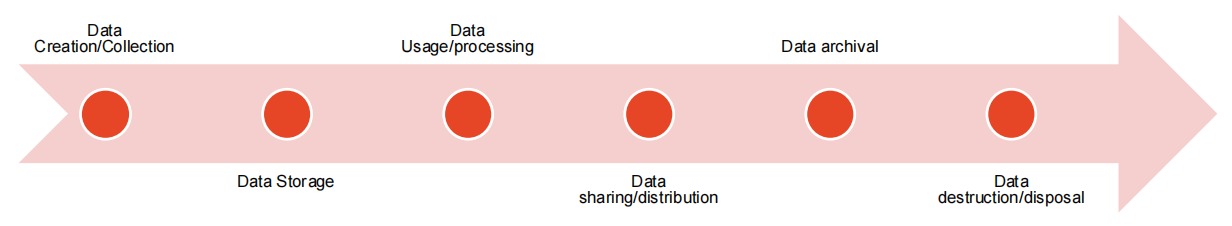
\includegraphics[width=0.9\linewidth]{figures/Week 10/Typical Data Lifecycle.png}
    \caption{A typical Data Lifecycle}
\end{figure}

\bigskip

\noindent\textbf{Data Creation/Collection}

Data is generated or collected from users, devices, or systems.

Examples: User registration forms, IoT sensors, employee records.

Security focus: Collect only necessary data (minimization). Secure input validation. Ensure informed consent at the point of collection.

\bigskip

\noindent \textbf{Data Storage}

Data is stored in databases, data warehouses, or cloud storage.

Security focus: Encryption at rest. Access controls (who can read/write). Redundancy and backups to prevent loss.

\bigskip

\noindent\textbf{Data Usage/Processing}

Data is used for operations, analytics, or decision-making.

Examples: HR system retrieving employee details, algorithms analyzing customer behavior.

Security focus: Encryption in use (confidential computing). Role-based access control. Audit logs of who accessed/modified data.

\bigskip

\noindent\textbf{Data Sharing/Distribution}

Data is shared internally (between departments) or externally (with partners, vendors, regulators).

Security focus: Encryption in transit (TLS/SSL, VPN). Data masking/anonymization for third parties. Contracts/agreements ensuring compliance with privacy laws.

\bigskip

\noindent\textbf{Data archival}

Data that’s no longer actively used but must be retained for compliance, historical, or business reasons.

Examples: Old financial records, patient health records.

Security focus: Secure long-term storage. Retrieval controls (only authorized users). Legal retention schedules (e.g., tax records for 7 years).

\noindent\textbf{Data Destruction/Disposal}

Data that’s no longer needed is securely destroyed.

Security focus: Shredding physical documents. Wiping/overwriting disks (DoD 5220.22-M, NIST standards). Cryptographic erasure in cloud environments.

\subsubsection{Security across the lifecycle}

\indent

At every stage, IT professionals must apply:

\begin{itemize}
    \item Confidentiality: Limit access to only those who need it.
    \item Integrity: Ensure data is accurate and not tampered with.
    \item Availability: Ensure authorized users can access data when required.
\end{itemize}

Data breaches often occur because organizations forget to protect “inactive” or “archived” data.

Regulations like GDPR require organizations to know where data is in its lifecycle.

Secure lifecycle management prevents unauthorized access, misuse, and legal non-compliance.

\subsection{Governance Frameworks}

\subsubsection{Governance Frameworks for Information Security}

\indent

\textbf{Information security governance} is about \textbf{establishing policies, procedures, and controls} so that information assets are protected and aligned with business objectives. 

Several widely-recognized frameworks help IT professionals do this.

A few examples of such frameworks are:

\begin{itemize}
    \item ITIL (Information Technology Infrastructure Library) - Covered in W6
    \item COBIT (Control Objectives for Information and related Technologies ) - W6
    \item NIST (National Institute of Standards and Technology)
    \item GDPR (General Data Protection Regulation)
\end{itemize}

\subsubsection{NIST Cybersecurity Framework (CSF)}

\indent

Origin: Developed by the National Institute of Standards and Technology (NIST), USA, primarily for critical infrastructure but widely adopted globally.

The main purpose of this framework was to:

\begin{itemize}
    \item Provide a risk-based approach to manage and improve cybersecurity.
    \item Be flexible enough to be adapted by organizations of all sizes and sectors.
\end{itemize}

Key benefits of NIST CSF:

\begin{itemize}
    \item Provides common language for cybersecurity discussions.
    \item Helps prioritize security investments based on risk exposure.
    \item Encourages continuous improvement.
\end{itemize}

The core components of NIST CSF are:

\begin{itemize}
    \item Framework Core (5 functions)
        \begin{itemize}
            \item Identify: Understand organizational assets, systems, data, and risks.
            \item Protect: Implement safeguards to limit or contain impact of cyber incidents.
            \item Detect: Identify cybersecurity events promptly.
            \item Respond: Act quickly to incidents to mitigate impact.
            \item Recover: Restore services and capabilities after an incident
        \end{itemize}
    \item Implementation Tiers
        \begin{itemize}
            \item Tier 1 (Partial): Cybersecurity is ad hoc and reactive, with informal or inconsistent practices.
            \item Tier 2 (Risk-informed): Cybersecurity policies exist but are applied inconsistently, with partial risk awareness.
            \item Tier 3 (Repeatable): Cybersecurity practices are formally documented, consistently applied, and monitored.
            \item Tier 4 (Adaptive): Cybersecurity is fully integrated, continuously improved, and adapts to evolving threats.
        \end{itemize}
    \item Profiles: Customized alignment of framework functions and categories with the organization’s business needs and risk tolerance.
\end{itemize}

\subsubsection{GDPR}

\indent 

Origin: European Union regulation, effective May 2018.

The main purpose for this regulation was to:

\begin{itemize}
    \item Protect the personal data and privacy rights of EU citizens.
    \item Standardize data protection laws across EU countries.
    \item Give individuals more control over their data.
\end{itemize}

Under this regulation, individuals have the following rights:

\begin{itemize}
    \item Right to access, rectify, erase, restrict processing, data portability, and object (covered in your “Individual Rights of Data” section).
    \item Right not to be subject to automated decision-making that significantly affects them.
\end{itemize}

Key principles of GDPR:

\begin{itemize}
    \item Lawfulness, Fairness, and Transparency: Data must be processed legally, fairly, and transparently.
    \item Purpose Limitation: Data collected for specific purposes only.
    \item Data Minimization: Collect only what’s necessary.
    \item Accuracy: Keep data accurate and up to date.
    \item Storage Limitation: Retain data only as long as necessary.
    \item Integrity and Confidentiality: Protect data against unauthorized access, loss, or damage.
    \item Accountability: Organizations must demonstrate compliance
\end{itemize}

\subsection{Cybersecurity Standards and Best practices}

\subsubsection{Cybersecurity}

\indent 

\textbf{Cybersecurity} is the practice of \textbf{protecting computers, networks, programs, and data from unauthorized access, attacks, damage, or theft.} It focuses specifically on the \textbf{digital aspect} of information security.

Cybersecurity is often aligned with the CIA Triad:

\begin{itemize}
    \item Confidentiality: Ensure that sensitive information is accessed only by authorized users.
    \item Integrity: Protect data from being altered or tampered with.
    \item Availability: Ensure systems and data are accessible to authorized users when needed.
\end{itemize}

\subsubsection{Domains of Cybersecurity}

\begin{itemize}
    \item \textbf{Network Security}: Protecting networks and connected devices from breaches and attacks.
    \item \textbf{Application Security}: Ensuring software is free of vulnerabilities and secure from threats.
    \item \textbf{Information Securit}y: Protecting data both at rest and in transit.
    \item \textbf{Operational Security (OPSEC)}: Policies and procedures to protect organizational processes.
    \item \textbf{Endpoint Security}: Protecting devices like computers, smartphones, and IoT devices.
    \item \textbf{Cloud Security}: Securing cloud-based infrastructure, applications, and data.
    \item \textbf{Identity \& Access Management (IAM)}: Controlling who can access what resources
\end{itemize}

\subsubsection{Common Cybersecurity Practices}

\begin{itemize}
    \item Use \textbf{strong passwords} and \textbf{multi-factor authentication (MFA)}.
    \item Keep software and systems \textbf{updated and patched}.
    \item Implement \textbf{firewalls, VPNs, and intrusion detection systems}.
    \item \textbf{Encrypt data} in transit and at rest.
    \item Train staff on \textbf{phishing, social engineering, and safe online behavior}.
    \item Develop an \textbf{incident response plan} for security breaches.
    \item Regularly \textbf{monitor systems and audit logs} for suspicious activity.
\end{itemize}

\subsubsection{Cybersecurity Standards}

\indent 

Cybersecurity standards provide organizations with structured guidelines, best practices, and controls to protect their digital assets. They help ensure consistency, compliance, and risk management across industries.

A few common cybersecurity standards are:

\begin{itemize}
    \item ISO/IEC 27001
    \item NIST Cybersecurity Framework
    \item PCI DSS (Payment Card Industry Data Security Standard)
    \item HIPAA Security Rule (Healthcare)
\end{itemize}

\subsubsection{PCI DSS – Payment Card Industry Data Security Standard}

\indent

The main purpose is to: Protect payment card data and reduce the risk of fraud for organizations that store, process, or transmit credit/debit card information. Developed by the PCI Security Standards Council (founded by Visa, MasterCard, Amex, Discover, and JCB).

The scope of this standard: Applies to any organization involved in payment card transactions, including merchants, processors, and service providers.

Key requirements of PCI DSS:

\begin{itemize}
    \item \textbf{Build and maintain a secure network}: Install and maintain a firewall to protect cardholder data. Do not use vendor-supplied default passwords.
    \item \textbf{Protect cardholder data}: Encrypt data in storage and in transit.
    \item \textbf{Maintain a vulnerability management program}: Use anti-virus and regularly update software.
    \item \textbf{Implement strong access control measures}: Restrict access to cardholder data by need-to-know. Assign unique IDs to users.
    \item \textbf{Monitor and test networks regularly}: Track and monitor all access to network resources and cardholder data. Regularly test security systems.
    \item \textbf{Maintain an information security policy}: Establish policies for employees and contractors.
\end{itemize}

\subsubsection{HIPAA – Health Insurance Portability and Accountability Act}

\indent 

The main purpose of this act is to: Protect \textbf{electronic protected health information (ePHI)} in the \textbf{healthcare industry}. Ensures confidentiality, integrity, and availability of patient health data.

The scope of this act: Applies to covered entities (healthcare providers, health plans, clearinghouses) and business associates (service providers handling ePHI).

Consequences of non-compliance: Civil penalties: \$100–\$50,000 per violation, up to \$1.5 million annually. Criminal penalties for knowingly violating HIPAA. Loss of reputation and patient trust.

HIPAA Security Rule Safeguards:

\begin{itemize}
    \item Administrative Safeguards
        \begin{itemize}
            \item Security management processes (risk analysis and mitigation).
            \item Workforce training on privacy and security policies.
            \item Contingency planning and incident response.
        \end{itemize}
    \item Physical Safeguards
        \begin{itemize}
            \item Facility access controls.
            \item Secure storage for servers, workstations, and paper records.
            \item Policies for device and media handling.
        \end{itemize}
    \item Technical Safeguards
        \begin{itemize}
            \item Access controls (unique IDs, passwords, and role-based access).
            \item Audit controls (tracking system activity).
            \item Integrity controls (ensure data is not improperly altered).
            \item Encryption of ePHI in storage and transmission.
        \end{itemize}
\end{itemize}

\subsection{Threat Modeling and Incident Response}

\subsubsection{Threat Modelling}

\indent 

Threat modelling is a \textbf{structured approach to identifying, understanding, and prioritizing potential security threats} to a system, application, or organization. It helps \textbf{anticipate attacks before they happen}.

The main purpose of threat modelling is to:

\begin{itemize}
    \item Identify \textbf{vulnerabilities} in systems or processes.
    \item Prioritize security measures based on \textbf{risk and potential impact}.
    \item Improve \textbf{design and architecture} with security in mind.
\end{itemize}

\subsubsection{STRIDE – Threat Modelling framework}

\indent 

STRIDE is a systematic framework for identifying security threats in software systems, applications, and IT infrastructure. It stands for 6 types of threats:

\begin{itemize}
    \item Spoofing Identity (S): When an attacker \textbf{pretends to be someone else} to gain unauthorized access.
    \item Tampering with Data (T): Unauthorized \textbf{modification of data} in storage, transit, or during processing.
    \item Repudiation (R): When a user \textbf{denies performing an action}, and the system lacks proof to dispute it.
    \item Information Disclosure (I): Unauthorized \textbf{exposure of sensitive information}.
    \item Denial of Service (D): Attacks that \textbf{make a system or service unavailable} to legitimate users.
    \item Elevation of Privilege (E): When a user or process \textbf{gains higher privileges} than intended
\end{itemize}

\subsubsection{Mitigation Strategies for STRID}

\begin{table}[h!]
\centering
\begin{tabular}{cl}
\hline
\textbf{Threat}                     & \multicolumn{1}{c}{\textbf{Mitigation Strategies}}                                                                                                              \\ \hline
\textbf{Spoofing Identity (S)}      & \begin{tabular}[c]{@{}l@{}}Multi-factor authentication (MFA)\\ Strong identity verification\\ Secure token-based authentication\end{tabular}                    \\
\textbf{Tampering with Data (T)}    & \begin{tabular}[c]{@{}l@{}}Digital signatures and checksums\\ Encryption of data in transit and at rest\\ Access controls with audit logs\end{tabular}          \\
\textbf{Repudiation (R)}            & \begin{tabular}[c]{@{}l@{}}Logging and audit trails\\ Non-repudiation mechanisms like digital signatures\\ Immutable storage for critical logs\end{tabular}     \\
\textbf{Information Disclosure (I)} & \begin{tabular}[c]{@{}l@{}}Encryption of sensitive data\\ Data classification and masking\\ Strong access controls and network segmentation\end{tabular}        \\
\textbf{Denial of Service (D)}      & \begin{tabular}[c]{@{}l@{}}Rate limiting and throttling\\ Load balancing and redundancy\\ Monitoring and automated alerting\end{tabular}                        \\
\textbf{Elevation of Privilege (E)} & \begin{tabular}[c]{@{}l@{}}Principle of least privilege (PoLP)\\ Regular patching and vulnerability management\\ Role-based access controls (RBAC)\end{tabular} \\ \hline
\end{tabular}
\end{table}

\subsubsection{Incident Response Plan}

\indent 

An \textbf{Incident Response Plan} is a \textbf{structured approach for detecting, responding to, and recovering from cybersecurity incidents}. It ensures that organizations \textbf{minimize damage, restore operations quickly, and meet legal and regulatory obligations}.

The main goal of an IRP is to:

\begin{itemize}
    \item Reduce \textbf{impact of cyber incidents} (financial, operational, reputational).
    \item Ensure \textbf{business continuity}.
    \item Learn from incidents to \textbf{improve future security posture}.
\end{itemize}

\subsubsection{Incident Response Lifecycle}

\indent 

\begin{itemize}
    \item Preparation
        \begin{itemize}
            \item Establish \textbf{policies, procedures, and tools} before an incident occurs.
            \item Train staff and \textbf{create an Incident Response Team (IRT)}.
            \item Implement monitoring and logging systems.
        \end{itemize}
    \item Identification
        \begin{itemize}
            \item Detect potential incidents \textbf{as early as possible}.
            \item Determine \textbf{scope, type, and severity} of the incident.
        \end{itemize}
    \item Containment
        \begin{itemize}
            \item \textbf{Limit the spread and impact} of the incident.
            \item \textbf{Short-term containment}: Immediate action to prevent further damage.
            \item \textbf{Long-term containment}: Implement fixes while maintaining operations
        \end{itemize}
    \item Eradication: \textbf{Remove the root cause} of the incident from the environment.
    \item Recovery
        \begin{itemize}
            \item \textbf{Restore affected systems and services} to normal operations.
            \item Ensure that systems are \textbf{fully functional, secure, and verified}.
            \item Monitor systems for \textbf{residual threats or recurring issues}.
        \end{itemize}
    \item Lessons Learned
        \begin{itemize}
            \item Conduct a \textbf{post-incident review}.
            \item Identify what went well? What could be improved? Gaps in policies or tech
            \item Update the \textbf{IRP, security controls, and employee training}.
            \item Document findings for \textbf{regulatory and audit purposes}.
        \end{itemize}
\end{itemize}

\subsubsection{Disaster Recovery Plan}

\indent 

A \textbf{Disaster Recovery Plan (DRP)} is a documented, structured approach that outlines \textbf{how an organization will recover IT systems, data, and operations after a disruptive event}, such as a cyberattack, hardware failure, natural disaster, or human error.

The goal is to:

\begin{itemize}
    \item \textbf{Minimize downtime} and data loss.
    \item \textbf{Ensure business continuity}.
    \item Protect critical systems and resources.
    \item Meet \textbf{regulatory and contractual requirements}.
\end{itemize}

\subsubsection{Disaster Recovery Strategies}

\begin{itemize}
    \item \textbf{Cold Site}: Pre-prepared physical location with basic infrastructure; requires setup during disaster.
    \item \textbf{Warm Site}: Partially equipped backup site; servers and data need configuration before use.
    \item \textbf{Hot Site}: Fully operational duplicate environment; can take over immediately during disaster.
    \item \textbf{Cloud-Based DR / DRaaS (Disaster Recovery as a Service)}: Replicate systems/data to cloud for rapid recovery.
    \item \textbf{Backup and Restore}: Regular backups stored offsite; slower recovery but cost-effective.
\end{itemize}

\bigskip

\noindent\textbf{Difference between IRP and DRP}

\begin{table}[h!]
\centering
\renewcommand{\arraystretch}{1.35}
\begin{tabular}{|p{3cm}|p{6.2cm}|p{6.2cm}|}
\hline
\textbf{Feature} & \textbf{Disaster Recovery Plan (DRP)} & \textbf{Incident Response Plan (IRP)} \\
\hline

\textbf{Focus} & Restoring IT systems, data, and operations after a disaster &
Detecting, containing, and mitigating cybersecurity incidents \\
\hline

\textbf{Objective} & Minimize downtime and data loss &
Minimize damage and contain threats \\
\hline

\textbf{Scope} & IT infrastructure, applications, backups &
Security incidents, breaches, attacks \\
\hline

\textbf{Timing} & Post-disaster recovery &
During and immediately after an incident \\
\hline

\textbf{Best Practices} &
\begin{itemize}
    \item Test the plan at least annually, or after major infrastructure changes
    \item Use redundancy and failover mechanisms (servers, networks, power supply)
    \item Maintain clear documentation accessible to authorized personnel
    \item Ensure regulatory compliance for data protection and recovery
    \item Align DRP with Incident Response Plan (IRP) and Business Continuity Plan (BCP)
\end{itemize}
&
\begin{itemize}
    \item Keep the plan up-to-date with evolving threats
    \item Conduct regular drills and tabletop exercises
    \item Use automated monitoring and alerting for faster detection
    \item Apply the principle of least privilege in access control
    \item Maintain offsite backups and redundant systems
    \item Integrate threat intelligence to anticipate attacks
\end{itemize}
\\
\hline

\end{tabular}
\caption{Difference between Disaster Recovery Plan (DRP) and Incident Response Plan (IRP)}
\end{table}

\subsubsection{Business Continuity Plan}

\indent 

A \textbf{Business Continuity Plan} is a \textbf{proactive strategy and documented plan} that ensures an organization can \textbf{continue essential operations during and after a disruptive event}, whether it’s a cyberattack, natural disaster, equipment failure, or other crises.

The main goal is to:

\begin{itemize}
    \item Maintain \textbf{critical business functions} during disruptions.
    \item Minimize \textbf{financial, operational, and reputational impact}.
    \item Ensure \textbf{employee, customer, and stakeholder confidence}.
    \item Complement \textbf{Disaster Recovery (DRP)} for IT systems.
\end{itemize}

\subsubsection{BCP Lifecycle}

\begin{itemize}
    \item \textbf{Project Initiation and Management}: Establish objectives, scope, and resources.
    \item \textbf{Business Impact Analysis (BIA)}: Identify critical functions and prioritize recovery.
    \item \textbf{Risk Assessment}: Evaluate threats and vulnerabilities.
    \item \textbf{Strategy Development}: Define recovery strategies for critical processes.
    \item \textbf{Plan Development}: Document procedures, roles, and resources.
    \item \textbf{Testing and Exercises}: Conduct drills to validate the plan.
    \item \textbf{Maintenance and Continuous Improvement}: Update plan based on lessons learned and changes in business.
\end{itemize}

\subsubsection{Best practices for BCP}

\begin{itemize}
    \item Align BCP with \textbf{DRP and IRP} for a complete resilience strategy.
    \item Identify and protect \textbf{key resources}, including staff, technology, facilities, and suppliers.
    \item Ensure \textbf{communication plans} are tested and accessible.
    \item Perform \textbf{regular audits and plan updates}.
    \item Use \textbf{cloud services and remote capabilities} to increase flexibility.
    \item Involve \textbf{leadership support} for faster decision-making during crises.
\end{itemize}

\subsection{Modern IT Security}

\indent 

Modern threats are evolving rapidly and often target humans, technology, and processes simultaneously. Security is no longer just IT’s responsibility, it requires an organization-wide approach. Proactive, layered defense using policies, technology, awareness, and continuous monitoring is essential. Integration of cybersecurity frameworks and standards (like NIST, ISO 27001, PCI DSS, HIPAA) is critical for resilience.

\subsubsection{Modern IT Security Challenges}

\begin{itemize}
    \item Cloud adoption risks
        \begin{itemize}
            \item Challenge: Increased attack surface due to distributed workforce and BYOD (Bring Your Own Device).
            \item Key issues may include misconfigurations, shared responsibility confusion, API vulnerabilities, etc.
        \end{itemize}
    \item Remote work security challenges
        \begin{itemize}
            \item Challenge: Increased attack surface due to distributed workforce and BYOD (Bring Your Own Device).
            \item Key issues may include usage of unsecured home networks, lack of enterprise security controls on personal devices, etc.
        \end{itemize}
    \item Shadow IT Challenge: Employees using unauthorized applications or cloud services without IT oversight.
\end{itemize}

\subsubsection{Cloud Deployment Models}

\begin{table}[htbp]
\centering
\renewcommand{\arraystretch}{1.3}
\begin{tabular}{|p{3.2cm}|p{7cm}|p{4.5cm}|}
\hline
\textbf{Model} & \textbf{Description} & \textbf{Example} \\
\hline

\textbf{Public Cloud} &
Services offered over the internet by third-party providers; shared infrastructure &
AWS, Microsoft Azure, Google Cloud \\
\hline

\textbf{Private Cloud} &
Cloud infrastructure dedicated to a single organization; more control and security &
VMware vSphere, OpenStack \\
\hline

\textbf{Hybrid Cloud} &
Combines public and private clouds; flexible workload distribution &
On-premises + Azure/AWS integration \\
\hline

\textbf{Community Cloud} &
Shared infrastructure for a specific group or industry &
Government or healthcare consortia clouds \\
\hline

\end{tabular}
\caption{Cloud Deployment Models}
\end{table}

\subsubsection{Cloud Service Models}

\begin{table}[htbp]
\centering
\renewcommand{\arraystretch}{1.3}
\begin{tabular}{|p{4cm}|p{7.2cm}|p{4cm}|}
\hline
\textbf{Model} & \textbf{Description} & \textbf{Example} \\
\hline

\textbf{Infrastructure as a Service (IaaS)} &
Provides virtualized computing resources (servers, storage, network) &
AWS EC2, Google Compute Engine \\
\hline

\textbf{Platform as a Service (PaaS)} &
Provides platform for application development and deployment &
Google App Engine, Microsoft Azure App Service \\
\hline

\textbf{Software as a Service (SaaS)} &
Provides fully managed software accessible via web &
Microsoft 365, Salesforce, Zoom \\
\hline

\textbf{Function as a Service (FaaS) / Serverless} &
Runs code without managing servers; triggered by events &
AWS Lambda, Azure Functions \\
\hline

\end{tabular}
\caption{Cloud Service Models}
\end{table}

\subsubsection{Security for Cloud and Virtualised Environments}

\indent 

Cloud and virtualization introduce \textbf{flexibility and scalability}, but they also create \textbf{new security challenges}. Security must cover \textbf{infrastructure, platforms, applications, and data} across \textbf{public, private, and hybrid environments}.

A few emerging security technologies are:

\begin{itemize}
    \item \textbf{Zero Trust Architecture}: “Never trust, always verify” for cloud users and devices.
    \item \textbf{Container Security}: Protect Kubernetes and Docker environments.
    \item \textbf{Cloud Workload Protection Platforms (CWPP)}: Monitor VMs, containers, and serverless workloads.
    \item \textbf{AI-Driven Threat Detection}: Detect anomalous behavior in cloud traffic.
\end{itemize}

\subsubsection{Cloud environment security best practices}

\begin{itemize}
    \item \textbf{Secure the Hypervisor}: Only authorized personnel access; patch regularly.
    \item \textbf{Encrypt Data}: At rest, in transit, and during backup.
    \item \textbf{Strong Identity Management}: RBAC, MFA, SSO for cloud access.
    \item \textbf{Monitor Logs and Network Traffic}: Centralized logging, SIEM integration.
    \item \textbf{Micro-Segmentation}: Limit lateral movement in virtual networks.
    \item \textbf{Regular Vulnerability Assessments}: Scan VMs, containers, and cloud workloads.
    \item \textbf{Secure Configuration}: Follow vendor-recommended security baselines (CIS benchmarks).
    \item \textbf{Automated Security Tools}: Use Cloud Security Posture Management (CSPM) and container security solutions.
\end{itemize}

\subsection{Questions}

\subsubsection{End of Lecture Questions}

\begin{itemize}
    \item Describe the data life cycle and explain why each stage needs protection.
    \item What is the difference between NIST and GDPR frameworks in security management?
    \item List common cyber-security practices to protect an organization from threats.
    \item Explain the difference between incident response, disaster recovery, and business continuity plans.
    \item What are the main cloud deployment and service models, and how do they differ?
    \item Name at least three modern IT security challenges introduced by cloud adoption and remote work.
\end{itemize}

\subsubsection{Case Study}

\indent 

CloudSafe Corp is a mid-sized company providing SaaS solutions for healthcare providers. The company recently migrated 70\% of its applications to a hybrid cloud model while keeping sensitive patient records on a private cloud. Employees are working remotely, and collaboration occurs via Slack, Microsoft Teams, and cloud storage.

Incident: One morning, the IT team detects abnormal activity: a ransomware strain has encrypted several production servers in the public cloud. Several employees report being unable to access shared files. The attack appears to have entered via a phishing email targeting remote employees, exploiting weak MFA implementation. Some VMs hosting the SaaS application are offline, impacting service delivery.

Current Status:

\begin{itemize}
    \item Private cloud data is safe but some hybrid cloud services are down.
    \item Incident response is partially executed, but some teams are unclear on responsibilities.
    \item Customers have reported outages, and media attention is rising
\end{itemize}

\noindent\textbf{Case Study based Questions}:

\begin{itemize}
    \item Identify at least three security failures that contributed to the ransomware attack.
    \item Explain how the hybrid cloud deployment model influenced the impact of this incident.
    \item What incident response steps should CloudSafe Corp implement immediately to contain the ransomware?
    \item Suggest backup and disaster recovery strategies for minimizing downtime in this scenario.
    \item Discuss the role of identity and access management (IAM) in preventing similar attacks.
    \item Design a high-level incident response checklist for CloudSafe Corp during a ransomware outbreak.
\end{itemize}
\pagebreak

\section{Week 11 - Ethics}
\indent

\textbf{Ethics} is the branch of philosophy that deals with what is right and wrong, good and bad, and how people should behave. It provides a framework for evaluating human actions, decisions, and intentions - especially when the right choice isn’t obvious.

In the professional IT context, Ethics refers to the \textbf{moral standards} that guide how IT professionals act when developing, managing, or using technology. It involves \textbf{responsible decision-making} - especially when those decisions affect people’s privacy, safety, or trust.

\subsection{Introduction}

\subsubsection{Key components of Ethics}

\indent 

\begin{itemize}
    \item Values: These are the deeply held beliefs or ideals that guide our decisions and shape what we consider right or wrong. Examples of core values include integrity, respect, responsibility, fairness, and trustworthiness.
    \item Principles: Principles are the general standards or rules derived from values that help us decide what actions are ethically acceptable. They provide structure - a moral compass that translates abstract values into concrete guidance. Examples of ethical principles in IT would be confidentiality, transparency, accountability, and non-maleficence.
    \item Behavior: Behavior is the observable expression of values and principles in real-life decisions and professional conduct. This is where ethics becomes visible - how professionals act when faced with a dilemma reveals their true ethical stance. Ethics is demonstrated through consistent behavior, not just belief.
    \item Consequences: Consequences are the results of our ethical (or unethical) actions. Evaluating consequences helps professionals understand whether their actions aligned with their intended ethical values.
\end{itemize}

\subsubsection{Our Ethical Framework}

\indent 

An \textbf{ethical framework} is a \textbf{structured way of thinking} about right and wrong. It helps professionals make \textbf{consistent, well-reasoned decisions}, especially when facing dilemmas where rules may be unclear or conflicting.

The IT world is full of \textbf{complex, high-impact decisions} - handling personal data, building AI models, managing automation, securing networks. Legal compliance alone isn’t enough; you often face situations where laws are silent or lag behind technology. A clear ethical framework ensures responsible innovation, public trust in technology, and professional accountability.

\subsubsection{Why Ethics matter in IT?}

\indent 

\begin{itemize}
    \item Technology shapes society: Information Technology now influences every part of modern life: communication, finance, healthcare, education, transportation, and even democracy. When IT professionals design systems, write algorithms, or process data, they’re shaping how people live and interact.
    \item IT Professionals handle sensitive information: Data is often described as the “new oil”, but it’s also deeply personal. Professionals in IT manage data that can reveal people’s habits, health, finances, and identities. Without ethical responsibility, that data can be misused, leaked, or sold without consent.
    \item Laws can't cover every situation: 
        \begin{itemize}
            \item Technology evolves faster than legislation. There are many situations where something is legal but not ethical, for example: Using publicly available data to profile users without consent. Automating layoffs using AI without human oversight.
            \item Ethics fills the gap between what is legal and what is right. It ensures professionals make responsible choices even when the law is silent or outdated.
        \end{itemize}
    \item Emerging technologies raise new ethical dilemmas
        \begin{itemize}
            \item As technologies like AI, Big Data, IoT, and automation advance, they raise novel ethical questions such as Who is responsible when an autonomous system fails? What biases are we embedding in AI systems?
            \item Ethics guides how we anticipate, design, and govern these technologies responsibly.
        \end{itemize}
\end{itemize}

\subsubsection{Laws vs Ethics}

\begin{table}[htbp]
\centering
\renewcommand{\arraystretch}{1.35}
\begin{tabular}{|p{3cm}|p{7cm}|p{7cm}|}
\hline
\textbf{Aspect} & \textbf{Laws} & \textbf{Ethics} \\
\hline

\textbf{Definition} &
\textbf{Laws are formal rules} established and enforced by governments or regulatory bodies. They define what is \textbf{legally permissible or punishable}. &
\textbf{Ethics refers to the moral principles and values} that govern an individual's or profession’s behavior. They go beyond legal compliance, asking what is \textbf{right, fair, and responsible}. \\
\hline

\textbf{Purpose} &
To maintain social order and justice &
To guide good and fair professional conduct \\
\hline

\textbf{Basis} &
Enforced by legal authority &
Driven by conscience and professional values \\
\hline

\textbf{Flexibility} &
Specific and fixed (can become outdated) &
Dynamic and adaptable to context \\
\hline

\textbf{Scope} &
Minimum acceptable standard of behavior &
Ideal standard of behavior (aspirational) \\
\hline

\end{tabular}
\caption{Comparison of Laws and Ethics}
\end{table}

\subsubsection{Core Ethical Principles in IT}

\indent 

Ethical principles act as moral guidelines that help IT professionals make responsible decisions when facing complex or ambiguous situations. They ensure that technology serves humanity fairly, safely, and transparently, aligning professional actions with both social good and individual responsibility.

The core principles are:

\begin{itemize}
    \item Integrity: Act honestly, consistently, and transparently in all professional dealings. In IT:
        \begin{itemize}
            \item Do not falsify data or manipulate analytics to satisfy management or clients.
            \item Accurately report project limitations, timelines, and risks.
            \item Maintain honesty even under pressure to deliver quick results.
        \end{itemize}
    \item Confidentiality and Privacy: Respect and protect the privacy and confidentiality of information entrusted to you. In IT:
        \begin{itemize}
            \item Protect sensitive data such as user credentials, financial records, or health information.
            \item Follow data minimisation principles - collect only what is necessary.
            \item Securely dispose of or anonymise data after use.
        \end{itemize}
    \item Fairness and Non-Discrimination: Treat all individuals and groups equitably, ensuring that technology does not perpetuate bias or inequality. In IT:
        \begin{itemize}
            \item Evaluate algorithms and datasets for bias or discrimination.
            \item Design accessible systems for all users, including those with disabilities.
            \item Avoid favoring certain users or clients unfairly.
        \end{itemize}
    \item Accountability and Responsibility: Accept responsibility for your actions, decisions, and the outcomes of the technology you develop or manage. In IT:
        \begin{itemize}
            \item Own up to mistakes and take corrective action quickly.
            \item Communicate potential risks or limitations to stakeholders.
            \item Follow due process for security disclosure or system failures.
        \end{itemize}
    \item Transparency and Honesty: Communicate clearly and openly about how systems work, what data they collect, and what limitations exist. In IT:
        \begin{itemize}
            \item Avoid hidden data practices or deceptive design (dark patterns).
            \item Inform users about how AI systems make decisions.
            \item Clearly document assumptions, models, and data sources.
        \end{itemize}
    \item Respect for Intellectual Property: Acknowledge and protect the ownership rights of others’ ideas, software, designs, and creative work. In IT:
        \begin{itemize}
            \item Do not copy or use others’ code, data, or algorithms without permission.
            \item Properly cite open-source material or licensed software.
            \item Respect software licenses and contribute ethically to collaborative projects.
        \end{itemize}
\end{itemize}

\subsubsection{ACS Code of Ethics}

\indent 

The Australian Computer Society (ACS) is the professional association 
for Australia’s ICT sector. All members are bound by the ACS Code of Professional Conduct, which establishes the ethical standards expected of ICT professionals in Australia.

The Code provides: A framework for ethical behavior; Guidance for decision-making when facing dilemmas; A basis for accountability to clients, employers, and society.

\begin{table}[htbp]
\centering
\renewcommand{\arraystretch}{1.35}
\begin{tabular}{|p{4.5cm}|p{10cm}|}
\hline
\multicolumn{2}{|c|}{\textbf{The 6 core values of the ACS Code of Ethics}} \\
\hline

\textbf{The Primacy of the Public Interest} &
Place the interests of the public above personal, business, or sectional interests. \\
\hline

\textbf{The Enhancement of Quality of Life} &
Strive to improve the quality of life of those affected by your work. \\
\hline

\textbf{Honesty} &
Be honest in your representation of skills, services, and products. \\
\hline

\textbf{Competence} &
Work competently and diligently for stakeholders. \\
\hline

\textbf{Professional Development} &
Enhance your own and others’ professional competence. \\
\hline

\textbf{Professionalism} &
Uphold and advance the honor and integrity of the profession. \\
\hline

\end{tabular}
\caption{ACS Code of Ethics: Six Core Values}
\end{table}

\subsection{Ethical Issues in IT}

\subsubsection{Privacy and Data Protection}

\indent 

Privacy and data protection involve ensuring that \textbf{personal, sensitive, or confidential data} is collected, stored, processed, and shared responsibly and lawfully.

Ethical principles involved: Primacy of public interest (ACS); Integrity, fairness, and accountability.

Ethical Questions:

\begin{itemize}
    \item Do users truly understand how their data is used?
    \item Should data be stored indefinitely “just in case”?
    \item Who is accountable for a data breach? the developer, manager, or company?
\end{itemize}

\subsubsection{Intellectual Property}

\indent

Intellectual property refers to \textbf{creations of the mind} - software, designs, algorithms, and other digital assets that are legally protected.

Ethical principles involved: Honesty, Competence, Professionalism

Ethical Questions:

\begin{itemize}
    \item Can you use AI-generated content that mimics another artist’s work?
    \item Should universities allow students to use ChatGPT for coding assignments?
\end{itemize}

\subsubsection{Cybersecurity responsibilities}

\indent

Cybersecurity ethics involve protecting \textbf{information systems and networks} against unauthorized access, misuse, or damage - while balancing privacy, freedom, and accountability.

Ethical principles involved: Public interest, Competence, Professionalism.

Ethical Questions:

\begin{itemize}
    \item Is it ethical to exploit a found vulnerability to “teach” a company a lesson?
    \item Do users have a right to know if their systems are unsafe?
\end{itemize}

\subsubsection{AI and Automation ethics}

\indent 

AI and automation ethics examine how intelligent systems \textbf{make decisions, impact society}, and \textbf{distribute responsibility} for outcomes.

Ethical principles involved: Public interest, Honesty, Quality of Life

Ethical Questions:

\begin{itemize}
    \item Who is accountable for AI’s actions? the developer or the algorithm?
    \item Should AI ever make life-and-death decisions (e.g., self-driving cars)?
\end{itemize}

\subsubsection{Workplace ethics in IT}

Workplace ethics covers professional behavior, communication, and conduct within IT organisations - ensuring respect, fairness, and accountability among colleagues and clients.

Ethical principles involved: Professionalism, Honesty, Enhancement of Quality of Life

Ethical Questions:

\begin{itemize}
    \item How do you respond when asked to “cut corners” on testing to meet deadlines?
    \item Should you report unethical behavior by a superior?
\end{itemize}

\subsection{Professional Code of Ethics}

\indent 

A \textbf{Professional Code of Ethics} is a \textbf{formal set of principles and standards} that guide the \textbf{behavior, decision-making, and conduct} of professionals within a specific field.

It defines what is considered \textbf{ethical and responsible behavior} and ensures that professionals act with \textbf{integrity, competence, and respect} toward clients, colleagues, and society.

The ICT industry impacts \textbf{privacy, safety, security, and equality} on a massive scale. A Professional Code of Ethics ensures that practitioners:

\begin{itemize}
    \item Use technology responsibly
    \item Avoid misuse of power or information
    \item Protect the public and environment
    \item Promote fairness, honesty, and respect
\end{itemize}

\subsubsection{ACS Code of Professional Conduct}

The \textbf{Australian Computer Society (ACS)} is Australia’s peak professional body for ICT practitioners. Its \textbf{Code of Professional Conduct} defines the \textbf{ethical and professional standards} expected from all ACS members - including students, graduates, and professionals.

The main purpose of the ACS Code is to ensure members:

\begin{itemize}
    \item Protect the \textbf{public interest} and promote social good
    \item Demonstrate \textbf{honesty, fairness, and integrity}
    \item Maintain \textbf{competence and accountability}
    \item Respect \textbf{privacy, confidentiality, and intellectual property}
    \item Promote \textbf{diversity, equity, and inclusion} in ICT workplaces
\end{itemize}

\begin{table}[htbp]
\centering
\renewcommand{\arraystretch}{1.35}
\begin{tabular}{|p{3cm}|p{7cm}|p{7cm}|}
\hline
\textbf{Aspect} & \textbf{ACS Code of Ethics} & \textbf{ACS Code of Professional Conduct} \\
\hline

\textbf{Nature} &
High-level moral principles &
Detailed professional rules \\
\hline

\textbf{Purpose} &
Guides ethical thinking and decision-making &
Guides enforceable professional behaviour \\
\hline

\textbf{Scope} &
Aspirational / Ideal &
Practical / Actionable \\
\hline

\textbf{Enforcement} &
Not strictly enforceable &
Enforceable; breaches can lead to sanctions \\
\hline

\textbf{Focus} &
Morality, public good, fairness &
Accountability, competence, professionalism \\
\hline

\textbf{Example} &
Anonymising user data to protect privacy &
Disclosing a security flaw per professional obligation \\
\hline

\end{tabular}
\caption{Comparison of ACS Code of Ethics and ACS Code of Professional Conduct}
\end{table}

\subsubsection{Personal vs Professional Ethics}

\indent 

Ethics can be applied at multiple levels.  In IT, it’s important to distinguish between personal ethics (your own moral compass) and professional ethics (standards required by your profession).

\begin{itemize}
    \item Personal Ethics: Personal ethics are an individual’s own moral values, principles, and beliefs about right and wrong. They are shaped by culture, religion, upbringing, and personal experiences.
    \item Professional Ethics: Professional ethics are the accepted standards of behavior for a specific profession. They are formalised in codes of conduct or codes of ethics (e.g., ACS Code of Professional Conduct).
\end{itemize}

Personal ethics influence professional ethics, but they must align with professional standards when on the job. Conflicts may arise, and professionals must balance personal beliefs with professional obligations.

Example:

Personal belief: “It’s fine to experiment on user data if it helps innovation.”

Professional obligation: ACS Code requires informed consent and privacy protection.

\subsection{Ethical Decision Making Models}

\indent 

\subsubsection{Consequentialism (Utilitarianism)}

Consequentialism is an ethical theory that \textbf{judges the morality of an action based on its outcomes or consequences}. The most well-known form of consequentialism is \textbf{Utilitarianism}.

Key features:

\begin{itemize}
    \item Outcome oriented: The \textbf{moral worth} of an action depends entirely on its results, not on intent or rules.
    \item Maximising good: Actions are judged by how much \textbf{overall good or utility} they produce (happiness, wellbeing, benefit).
    \item Impartiality: All affected parties’ interests are considered equally.
\end{itemize}

Strengths:

\begin{itemize}
    \item Practical: Focuses on real-world outcomes.
    \item Flexible: Can adapt to different contexts and technologies.
    \item Outcome-driven: Useful for risk-benefit analysis in IT projects.
\end{itemize}

Limitations:

\begin{itemize}
    \item Hard to predict all consequences accurately.
    \item May justify unethical means if the outcome seems beneficial (“ends justify the means”).
    \item Can conflict with personal or professional rules (e.g., privacy laws).
\end{itemize}

\subsubsection{Deontological (Duty-based)}

\indent 

Deontological ethics is an ethical theory that \textbf{focuses on the inherent rightness or wrongness of actions}, rather than their outcomes. It is also called \textbf{duty-based ethics}, because it emphasizes \textbf{adhering to moral rules, duties, or obligations}.

Key features:

\begin{itemize}
    \item Rule oriented: Actions are guided by \textbf{universal moral rules} or professional duties.
    \item Intent matters: The motive or intention behind the action is ethically significant.
    \item Consistency: Ethical rules apply \textbf{consistently to everyone}, independent of context or outcomes.
\end{itemize}

Strengths:

\begin{itemize}
    \item Provides \textbf{clear guidance}: rules are explicit and easy to follow.
    \item Emphasizes \textbf{moral integrity and accountability}.
    \item Aligns well with professional codes and legal compliance.
\end{itemize}

Limitations:

\begin{itemize}
    \item Can be rigid: may lead to outcomes that seem harmful or impractical.
    \item Conflicts may arise when duties clash (e.g., confidentiality vs. public safety).
    \item Less flexible for complex, real-world technological dilemmas.
\end{itemize}

\subsubsection{Virtue Ethics}

\indent 

Virtue Ethics is an ethical theory that \textbf{focuses on the character, moral virtues, and integrity of the individual}, rather than rules (deontology) or outcomes (consequentialism). It asks “\textbf{What kind of professional should I be}?” rather than just “What should I do?

Key features:

\begin{itemize}
    \item Character centric: Emphasizes cultivating \textbf{moral virtues} such as honesty, courage, integrity, fairness, and empathy.
    \item Habitual good conduct: Ethical behavior is a result of \textbf{developing good habits} over time.
    \item Practical wisdom: Professionals use judgment to navigate complex situations, balancing virtues appropriately.
\end{itemize}

Strengths:

\begin{itemize}
    \item Encourages \textbf{holistic moral development} of professionals.
    \item Flexible: considers context and nuance.
    \item Complements rules and outcomes - it promotes \textbf{ethical culture}, not just compliance.
\end{itemize}

Limitations

\begin{itemize}
    \item Less prescriptive: doesn’t provide explicit instructions for specific dilemmas.
    \item Can be \textbf{subjective} - what counts as a “virtue” may vary by culture or workplace.
    \item Requires \textbf{self-reflection and moral judgment}, which can be inconsistent.
\end{itemize}

\subsubsection{Ethics in Emerging technologies}

\indent 

Emerging technologies like \textbf{AI, Big Data, IoT, Cloud Computing, and Deepfakes} are reshaping society, but they bring \textbf{new ethical challenges}. ICT professionals must balance \textbf{innovation with responsibility}.

Ethical concerns:

\begin{itemize}
    \item Artificial Intelligence
        \begin{itemize}
            \item Algorithmic bias: AI may reinforce social inequalities.
            \item Transparency: “Black box” models make decisions difficult to explain.
            \item Accountability: Who is responsible if AI causes harm?
            \item Privacy: AI often requires large datasets that may include personal information.
        \end{itemize}
    \item Big Data
        \begin{itemize}
            \item Data privacy: Collection, storage, and sharing of massive datasets.
            \item Consent: Users may not understand how their data is used.
            \item Misuse: Predictive analytics could lead to discrimination (e.g., in hiring or insurance).
        \end{itemize}
    \item Internet of Things
        \begin{itemize}
            \item Security vulnerabilities: Devices can be hacked, exposing personal data.
            \item Surveillance: Continuous monitoring can infringe on privacy.
            \item Data ownership: Who controls the data collected by smart devices?
        \end{itemize}
    \item Cloud Computing
        \begin{itemize}
            \item Data sovereignty: Data stored across countries may violate local laws.
            \item Access control: Shared cloud resources may be exploited by malicious actors.
            \item Vendor responsibility: Cloud providers must uphold ethical and legal standards.
        \end{itemize}
    \item Deepfakes and Synthetic Media
        \begin{itemize}
            \item Misinformation: Deepfakes can be used to deceive or manipulate public opinion.
            \item Consent: Using someone’s likeness without permission is unethical.
            \item Trust erosion: Widespread deepfakes may undermine trust in digital content.
        \end{itemize}
\end{itemize}

\subsubsection{Balancing Innovation and Responsibility}

\indent 

Emerging technologies \textbf{offer immense benefits} but also \textbf{introduce risks}. ICT professionals must \textbf{apply ethical frameworks, ACS principles, and decision-making models} to: Protect users and society; Avoid harm and bias; Promote transparency and accountability.


Guiding questions:

\begin{itemize}
    \item Who benefits and who could be harmed?
    \item Are there fairness, privacy, or consent issues?
    \item Does this comply with professional codes and laws?
    \item Are the long-term societal consequences acceptable?
\end{itemize}

\subsection{Questions}

\subsubsection{End of Lecture Questions}

\begin{itemize}
    \item Define ethics and explain the difference between personal ethics and professional ethics.
    \item List and briefly describe the six key principles of the ACS Code of Professional Conduct.
    \item Identify five major ethical issues in IT and provide a real-world example for each.
    \item Explain a scenario where intellectual property rights could conflict with workplace demands.
    \item Compare and contrast Consequentialism, Deontological Ethics, and Virtue Ethics.
    \item When might personal ethics conflict with professional ethics? How should a professional resolve such a conflict?
\end{itemize}

\subsubsection{Case Study}

\indent 

You are a software engineer at a mid-sized Australian tech company developing an AI-powered recruitment platform. The system screens resumes and ranks candidates based on predicted job performance.

During testing, you discover that the AI algorithm systematically favors male candidates over female candidates, even though the data input was intended to be gender-neutral. Management insists that the platform be launched immediately because several large clients are waiting.

You are now faced with multiple considerations:

\begin{itemize}
    \item Public Interest: Launching a biased system could harm job applicants and damage public trust.
    \item Company Pressure: Delaying the launch may hurt client relationships and revenue.
    \item Professional Standards: The ACS Code of Professional Conduct requires fairness, honesty, and acting in the public interest.
    \item Legal Compliance: Discrimination in hiring is prohibited under Australian law.
\end{itemize}

\bigskip

\noindent\textbf{Case Study based Questions}

\begin{itemize}
    \item What are the main ethical issues in this scenario?
    \item Which ACS Code principles are most relevant to this situation?
    \item Using Consequentialism (Utilitarianism), what should you do? Consider both positive and negative consequences.
    \item Using Deontological Ethics, what action would be ethically required?
    \item Using Virtue Ethics, how should your personal and professional character guide your decision?
    \item Propose a step-by-step approach to address the bias in the AI system while balancing ethical, legal, and business concerns.
    \item How does this case illustrate the importance of professional accountability in IT?
\end{itemize}
\pagebreak

\section{Week 12 - Data based Decision Making}
\subsection{Decision Making in IT}

\indent 

\textbf{Decision making} is the \textbf{process of selecting the best possible course of action} from a set of alternatives to achieve a desired goal or solve a problem.

It’s one of the most important skills in professional and organizational contexts, especially in \textbf{Information Technology (IT)}, where choices often have long-term technical, financial, and strategic impacts.

It is important in IT as IT professionals make \textbf{high-impact decisions}, from choosing technologies to managing projects and ensuring data security. \textbf{Data-based decision-making} leads to more \textbf{accurate, transparent, and efficient} outcomes. It reduces bias, supports innovation, and improves risk management.

\begin{figure}[htbp]
    \centering
    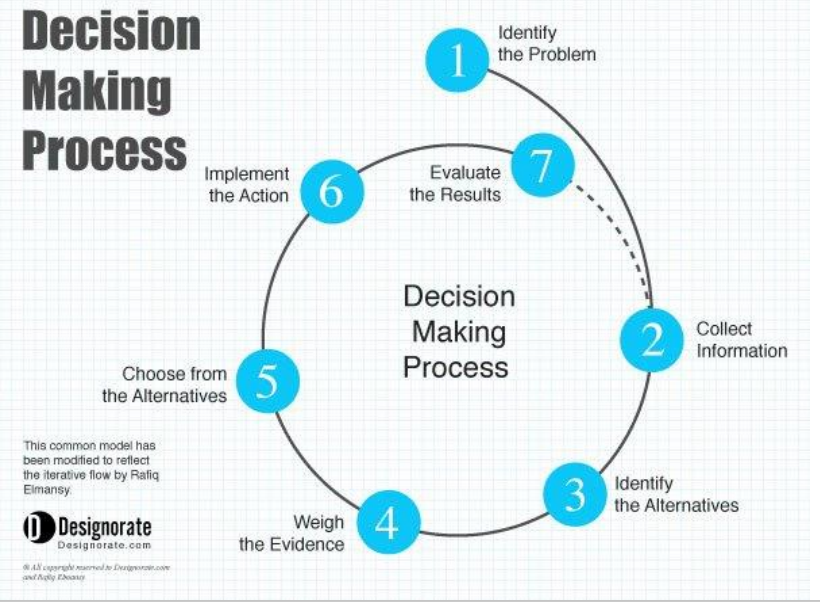
\includegraphics[width=0.7\linewidth]{figures/Week 12/DM Process.png}
\end{figure}

\begin{itemize}
    \item Identify the problem: The first step is to clearly define what needs to be decided or solved.
    \item Collect Information: Gather relevant \textbf{data, facts, and evidence} to understand the problem fully. This can include user analytics, system logs, financial reports, or stakeholder feedback.
    \item Identify the Alternatives: List possible courses of action or solutions. Good decision-making requires creative thinking and multiple options.
    \item Weigh the Evidence: Evaluate each alternative by considering \textbf{pros, cons, risks, and outcomes}. You may use decision matrices, SWOT analysis, or cost–benefit analysis.
    \item Choose from the Alternatives: Select the most suitable solution based on the evidence collected. This step combines \textbf{data-driven reasoning} with \textbf{professional judgment}.
    \item Implement the Action: Put the decision into action. This includes assigning tasks, allocating resources, and setting timelines.
    \item Evaluate the Results: Review the outcomes of the decision to see if it solved the problem or achieved the goal.
\end{itemize}

\subsubsection{Types of Decisions based on the Level of Management}

\indent 

Organisations make decisions at three key management levels:

\begin{itemize}
    \item Operational (Lower-level management): Operational decisions are routine, day-to-day choices that ensure the smooth functioning of an organisation’s ongoing activities. They typically deal with short-term goals and have low risk.
    \item Tactical (Middle management): Tactical decisions are medium-term, project- or department-level decisions that translate strategic goals into practical actions. They are semi-structured, combining data analysis with managerial judgment.
    \item Strategic (Top management): Strategic decisions are long-term, organization-wide decisions that define the direction, vision, and competitive advantage of the company. They are unstructured, high-risk, and have far-reaching consequences.
\end{itemize}

\begin{table}[htbp]
\centering
\renewcommand{\arraystretch}{1.35}
\begin{tabular}{|c|c|c|c|}
\hline
\textbf{Aspect} & \textbf{Operational Decision} & \textbf{Tactical Decisions} & \textbf{Strategic Decisions} \\
\hline

\textbf{Focus} &
Daily operations &
Project execution &
Long term vision \\
\hline

\textbf{Level} &
Supervisors / Technicians &
Manager / Team Leads &
Executives / Directors \\
\hline

\textbf{Time Frame} &
Short Term &
Medium Term &
Long Term \\
\hline

\textbf{Nature} &
Structured &
Semi-Structured &
Unstructured \\
\hline

\textbf{Data Type} &
Transactional, detailed &
Summarised reports &
Aggregated, predictive \\
\hline

\textbf{Risk} &
Low &
Moderate &
High \\
\hline

\end{tabular}
\caption{Types of Decisions Based on Management Levels}
\end{table}

\subsubsection{Rational vs Intuitive Decision Making}

\indent

\begin{table}[htbp]
\centering
\renewcommand{\arraystretch}{1.4}
\begin{tabular}{|c|p{6cm}|p{6cm}|}
\hline
\textbf{Aspect} & \textbf{Rational Decision Making} & \textbf{Intuitive Decision Making} \\
\hline

\textbf{Introduction} &
A logical, structured, and data-driven approach where decisions are made after careful analysis of facts, data, and alternatives. &
A spontaneous, experience-based process that relies on gut feeling, instincts, or professional judgment rather than analytical reasoning. \\
\hline

\textbf{Focus} &
Objectivity, evidence, and reasoning. &
Experience, pattern recognition, and tacit knowledge. \\
\hline

\textbf{Goal} &
Maximize outcomes by minimizing uncertainty through analysis. &
Make timely, confident decisions in uncertain or time-pressured situations. \\
\hline

\end{tabular}
\caption{Comparison of Rational vs Intuitive Decision Making}
\end{table}

\subsubsection{IT Specific Decision challenges}

\indent 

Every IT decision, from choosing a new software tool to designing a cybersecurity strategy, involves balancing \textbf{technical feasibility, business value, user experience, cost, and risk}.

IT decision-making is characterised by:

\begin{itemize}
    \item \textbf{High uncertainty}: due to evolving technologies and unpredictable project outcomes.
    \item \textbf{Complex interdependencies}: as one technical decision often impacts multiple systems or departments.
    \item \textbf{Rapid change cycles}: where decisions made today might need revision in months or even weeks.
    \item \textbf{Multi-stakeholder involvement}: requiring collaboration between technical experts, managers, and end-users.
    \item \textbf{Strong reliance on data}: supported by analytics, performance metrics, and 
predictive models.
\end{itemize}

\subsubsection{1. Rapid technological change}

\indent

Technology evolves faster than organizational policies, budgets, and skill sets can adapt. IT professionals often need to make decisions with \textbf{incomplete or rapidly changing information}.

Challenges:

\begin{itemize}
    \item Short technology lifecycles $\rightarrow$ risk of tools becoming obsolete.
    \item Pressure to adopt new tech (e.g., AI, blockchain, cloud computing) before fully understanding implications.
    \item Balancing innovation with stability.
\end{itemize}

Professional Insight: Use \textbf{technology roadmaps} and \textbf{proof-of-concept (POC)} evaluations to manage uncertainty and reduce risk

\subsubsection{2. Data driven vs Experience driven decision}

\indent 

Modern IT decisions rely heavily on data (metrics, analytics, KPIs), but \textbf{not all factors can be quantified}. Experienced professionals bring intuition and context that data might miss.

Challenges:

\begin{itemize}
    \item Over-reliance on data may ignore human or contextual insights.
    \item Over-reliance on intuition may introduce bias or errors.
    \item Conflicts between analytics teams and senior managers.
\end{itemize}

Professional Insight: The most effective IT leaders combine \textbf{quantitative data} with \textbf{qualitative judgment}.

\subsubsection{3. Security vs Usability trade-offs}

\indent

Every IT system faces a fundamental trade-off between \textbf{tight security} and \textbf{user convenience}. Stronger security often introduces complexity, while simplicity can reduce protection.

Challenges:

\begin{itemize}
    \item Balancing security compliance with user experience.
    \item Justifying security investments with limited budgets.
    \item Managing user resistance to strict controls.
\end{itemize}

Professional Insight: Adopt a \textbf{risk-based security model}, where the level of security matches the sensitivity of the system.

\subsection{Business Intelligence}

\textbf{Business Intelligence (BI)} refers to the \textbf{processes, technologies, and tools} that collect, integrate, analyze, and present \textbf{business data} to help organizations make \textbf{informed, data-driven decisions}.

In simple terms, BI turns \textbf{raw data into actionable insights}, enabling businesses to understand what’s happening, why it’s happening, and what to do next.

In modern organizations, \textbf{data is one of the most valuable assets}. However, data alone has little value unless it can be translated into insights that guide strategy and operations. That’s where \textbf{Business Intelligence} comes in.

\subsubsection{Business Intelligence vs Analytics vs Data Science}

\indent

\begin{table}[htbp]
\centering
\renewcommand{\arraystretch}{1.35}
\begin{tabular}{|p{3cm}|p{4cm}|p{4cm}|p{4cm}|}
\hline
\textbf{Aspect} &
\textbf{Business Intelligence} &
\textbf{Business Analytics} &
\textbf{Data Science} \\
\hline

\textbf{Primary Focus} &
\textbf{Descriptive understanding} – focuses on reporting, monitoring, and summarising existing data to understand \textit{what has happened} in the organisation. &
\textbf{Predictive and prescriptive analysis} – explores data trends, identifies patterns, and forecasts \textit{what is likely to happen or what should be done next}. &
\textbf{Discovery and automation} – uses advanced algorithms and machine learning to uncover hidden patterns and enable automated, data-driven actions. \\
\hline

\textbf{Purpose} &
To provide visibility and transparency into business operations through dashboards and reports. &
To provide deeper insights and strategic guidance by analyzing causes and predicting outcomes. &
To build intelligent systems and data products that can learn, adapt, and make predictions or decisions autonomously. \\
\hline

\textbf{Techniques} &
Reporting, dashboards, OLAP &
Statistical modeling, forecasting &
Machine learning, AI, NLP \\
\hline

\end{tabular}
\caption{Comparison of Business Intelligence, Business Analytics, and Data Science}
\end{table}

\subsubsection{BI Architecture \& Components}

\indent 

\textbf{BI Architecture} is a \textbf{structured framework} that defines how data flows from sources to actionable insights for decision-making. It ensures that \textbf{data is collected, transformed, stored, analyzed, and presented} efficiently to support both operational and strategic decisions. Think of it as the \textbf{pipeline that turns raw data into intelligence}.

\begin{figure}[htbp]
    \centering
    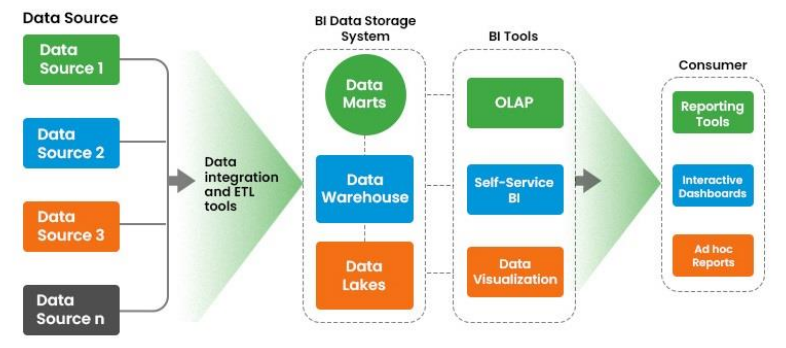
\includegraphics[width=0.8\linewidth]{figures/Week 12/BI Architure.png}
\end{figure}

\subsubsection{How BI supports Decision making?}

\begin{itemize}
    \item Provides Data-driven insights: BI systems collect and consolidate data from multiple sources such as sales, finance, marketing, operations, etc. This unified view eliminates guesswork.
        
        Impact: Managers can base decisions on facts and trends rather than intuition.
    \item Improves Decision speed and accuracy: Real-time dashboards and automated reports allow faster access to performance data.
        
        Impact: Enables timely decisions and proactive responses to business issues.
    \item Identifies trends and opportunities: BI tools use historical and current data to reveal emerging patterns.
        
        Impact: Helps businesses anticipate market changes, customer behavior, and growth opportunities.
\end{itemize}

\subsubsection{BI and IT Decision Challenges}

\begin{itemize}
    \item Data quality and accuracy: BI systems rely heavily on clean and accurate data. Inconsistent, incomplete, or duplicate data leads to misleading insights.
    \item Data integration: Organizations collect data from various systems (ERP, CRM, social media, IoT, etc.). Integrating these into one BI platform is complex.
    \item Data governance and security: BI systems deal with sensitive data that must comply with regulations (GDPR, HIPAA, etc.). Lack of governance leads to unauthorized access or compliance breaches.
    \item System integration with legacy platforms: Many businesses still run legacy systems incompatible with modern BI tools.
\end{itemize}

\subsubsection{Current Trends}


\begin{itemize}
    \item AI and Machine Learning Integration :BI tools are increasingly embedding AI/ML to generate insights, forecasts, and automate analysis. Features like natural-language query (NLQ), automated storytelling, anomaly detection are becoming standard. Organisations are also building \textbf{semantic layers} to make AI-powered BI more accurate and governed.
    \item Self-service BI \& Democratisation of Data: More business users (not just data specialists) are being empowered to explore data, build dashboards, and get insights. Low-code/no-code BI platforms are gaining traction.
    \item Real time analytics \& Edge computing: More use of streaming data, event-driven analytics, processing data at the “edge” (near data source) for low latency. Real-time dashboards and decisioning are increasingly expected.
\end{itemize}

\subsubsection{Future Challenges}

\begin{itemize}
    \item Managing Data explosion and complexity: The volume, velocity, and variety of data are growing exponentially (IoT, social media, sensors, AI models). BI systems must handle \textbf{structured, semi-structured, and unstructured data} at scale.
        
        Challenge: Designing architectures that can efficiently manage \textbf{real-time, multi-source, and massive datasets} without performance loss.
    \item Balancing AI automation with Human oversight: Modern BI increasingly uses AI for predictive and prescriptive analytics. However, \textbf{automated insights without human context} can lead to flawed or biased decisions.
        
        Challenge: Maintaining \textbf{explainability, transparency, and ethical governance} of AI-driven BI systems.
    \item Ensuring Data Ethics, Privacy, and Compliance: Data protection regulations (GDPR, CCPA, Australia’s Privacy Act) are becoming stricter. BI tools must comply while still enabling deep analysis.
        
        Challenge: Balancing \textbf{data accessibility with privacy}, and ensuring \textbf{ethical use} of data insights.
    \item Real-time Decision fatigue: With the rise of real-time analytics, organizations risk \textbf{information overload}. Constant data streams can overwhelm managers, leading to rushed or poor decisions.
        
        Challenge: Designing systems that provide \textbf{contextual, prioritized insights}, not raw data floods.
\end{itemize}

\subsection{BI Architecture}

\subsubsection{Data Sources Layer}

\indent 

The origin of all data. Data can come from multiple \textbf{internal and external sources}, structured or unstructured.

Purpose: Provide \textbf{raw information} for the BI system to process.

Types of Data Sources:

\begin{itemize}
    \item \textbf{Internal Systems}: ERP, CRM, HR systems, financial databases.
    \item \textbf{External Sources}: Social media, market reports, IoT sensors, web APIs.
    \item \textbf{Unstructured Data}: Emails, documents, audio/video files.
\end{itemize}

\subsubsection{ETL Layer (Extract, Transform, Load)}

\indent

ETL is the \textbf{process that collects, cleans, and prepares data} for analysis.

\textbf{Purpose}: Ensure \textbf{data quality, consistency, and usability}.

Steps:

\begin{itemize}
    \item \textbf{Extract}: Pull data from various sources.
    \item \textbf{Transform}: Clean, normalize, aggregate, and structure data.
    \item \textbf{Load}: Store transformed data into a data warehouse or data mart.
\end{itemize}

\subsubsection{Data Warehouse/Data Storage Layer}

\indent 

A \textbf{centralized repository} for storing \textbf{historical and structured data} from multiple sources.

\textbf{Purpose}: Provides \textbf{a single source of truth} for business reporting and analysis.

Key points:

\begin{itemize}
    \item Optimized for \textbf{querying and reporting}.
    \item Supports \textbf{OLAP (Online Analytical Processing)} for multidimensional analysis.
    \item May include \textbf{data marts} for specific departments (e.g., finance, sales, HR)
\end{itemize}

\subsubsection{OLAP \& Analytical Processing Layer}

\indent 

This layer allows \textbf{multi-dimensional data analysis} such as slicing, dicing, drilling down, rolling up, and pivoting, to uncover insights.

\textbf{Purpose}: Enable \textbf{interactive analysis and insights discovery}.

Key Features:

\begin{itemize}
    \item \textbf{Slicing}: View data for a specific dimension (e.g., sales by region).
    \item \textbf{Dicing}: Analyze data across multiple dimensions simultaneously.
    \item \textbf{Drill Down / Roll Up}: Move between detailed and summarized data.
    \item \textbf{Pivot}: Rotate data dimensions for alternative perspectives.
\end{itemize}

\subsubsection{BI Tools/Platforms}

\textbf{Business Intelligence (BI) tools} are software applications that \textbf{collect, process, analyze, and visualize} large volumes of business data to help organizations make data-driven decisions.

\subsection{OLAP Operations}

\subsubsection{Slicing}

\indent 

\begin{figure}[htbp]
    \centering
    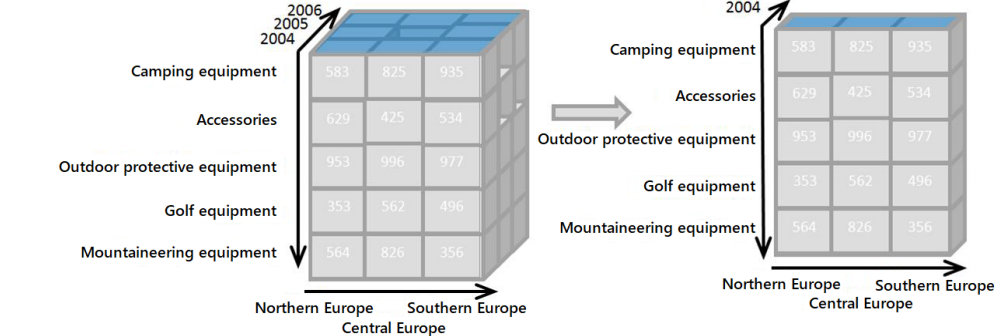
\includegraphics[width=0.8\linewidth]{figures/Week 12/Slicing.png}
    \caption{Slicing}
\end{figure}

Definition: Selects a single layer of data along one dimension of a cube.

Purpose: Focuses on a specific subset of data.

Example: Looking at sales data only for “2025” across all regions and products.

\subsubsection{Dicing}

\indent 

\begin{figure}[htbp]
    \centering
    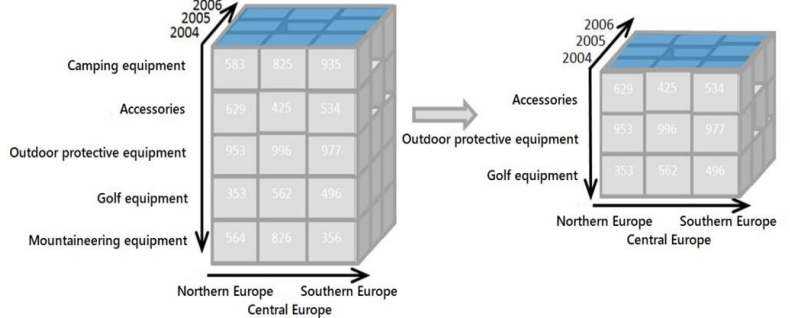
\includegraphics[width=0.8\linewidth]{figures/Week 12/Dicing.png}
    \caption{Dicing}
\end{figure}

Definition: Selects a sub-cube by choosing specific values across multiple dimensions.

Purpose: Analyzes data for multiple criteria at once.

Example: Viewing sales data for Region = Asia and Product = Laptop during Q1 2025.

\subsubsection{Drill Down}

\indent 

\begin{figure}[htbp]
    \centering
    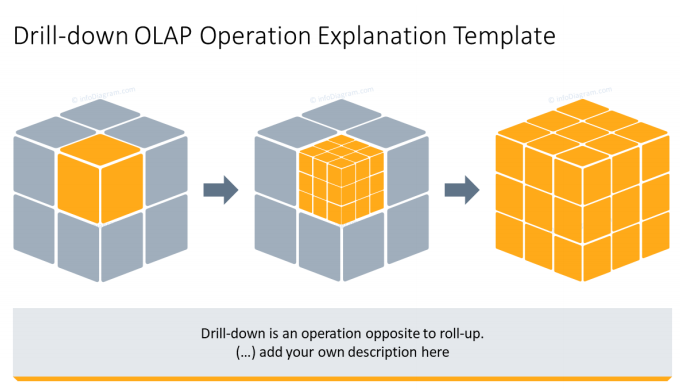
\includegraphics[width=0.6\linewidth]{figures/Week 12/Drill Down.png}
    \caption{Drill Down}
    \label{fig:placeholder}
\end{figure}

Definition: Moves from \textbf{summary data to more detailed data}.

Purpose: Understand granular details behind aggregated results.

Example: From quarterly sales totals to monthly or daily sales.

\subsubsection{Roll up}

\indent 

\begin{figure}[htbp]
    \centering
    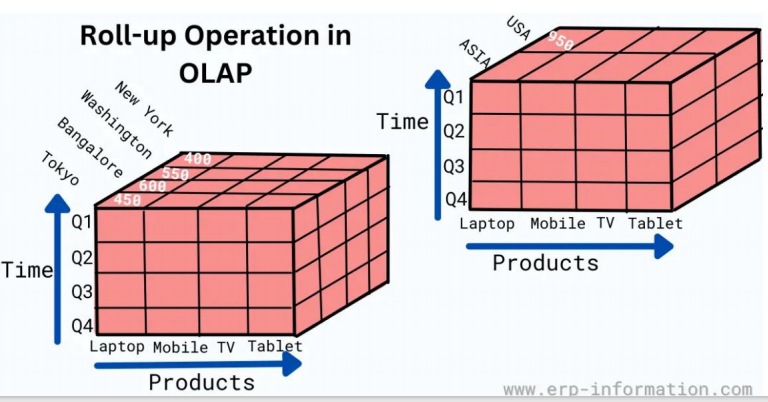
\includegraphics[width=0.7\linewidth]{figures/Week 12/Roll up.png}
    \caption{Roll up}
\end{figure}

Definition: Aggregates data from \textbf{a detailed level to a higher summary level}.

Purpose: Provides high-level overview or trend analysis.

Example: From daily sales → monthly sales → yearly sales.

\subsubsection{Pivot (Rotate)}

\indent 

\begin{figure}
    \centering
    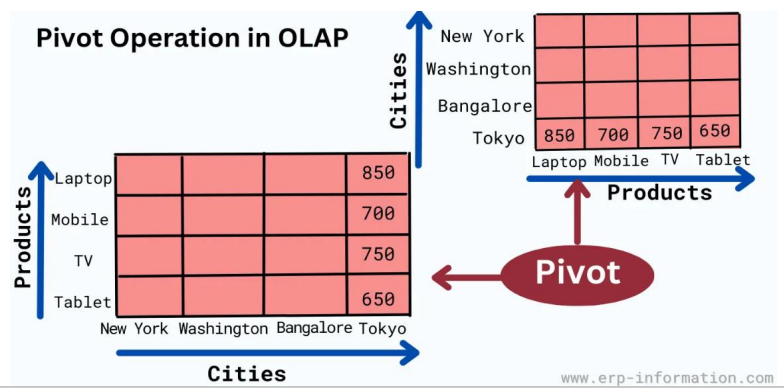
\includegraphics[width=0.7\linewidth]{figures/Week 12/Pivot (Rotate).png}
    \caption{Pivot (Rotate)}
\end{figure}

Definition: Reorients the data cube to \textbf{change the perspective}.

Purpose: Makes it easier to analyze relationships between dimensions.

Example: Swap rows and columns in a report: instead of Region as rows and Product as columns, you show Product as rows and Region as columns.

\subsection{Questions}

\subsubsection{End of Lecture Questions}

\begin{itemize}
    \item What is Business Intelligence (BI), and how does it differ from traditional data reporting?
    \item How does BI contribute to better decision-making across different management levels?
    \item How would you use BI to improve operational efficiency in a retail or healthcare setting?
    \item Define rational and intuitive decision making. In what situations is each approach more effective?
    \item Describe how decision making differs at the operational, tactical, and strategic levels of management.
    \item What strategies can be used to ensure ethical decision making when using AI or automated systems?
\end{itemize}

\subsubsection{Case Study}

\indent 

NovaTech Solutions is a mid-sized IT services company that recently implemented a Business Intelligence (BI) platform to improve its decision-making process.

Previously, departmental managers made decisions based on spreadsheets and personal judgment, leading to inconsistent outcomes. Now, the BI system integrates real-time data from sales, customer feedback, project performance, and financial systems.

During a quarterly review, the BI dashboard revealed that customer satisfaction scores had dropped by 15\% in the last two months. Further analysis showed delays in project delivery and increased staff turnover in the technical support team.

Management must now decide how to address these issues before they impact client retention and profitability

\bigskip

\noindent \textbf{Case Study based Questions}

\begin{itemize}
    \item Identify the type(s) of decision (operational, tactical, or strategic) that management needs to make in this situation. Explain your reasoning.
    \item How can NovaTech use its BI system to analyze the root causes of the declining customer satisfaction scores?
    \item What IT tools or techniques (e.g., dashboards, predictive analytics, data visualization) could help management make informed decisions?
    \item Discuss how a combination of rational and intuitive decision making might be used to solve the problem.
    \item What are two potential challenges NovaTech might face in relying on BI for decision making, and how could they overcome them?
\end{itemize}
\pagebreak

\section{Tutorial 2}
\subsection{PART A – Sources of Information}

\indent 

Go through the documentations under the section “Finding, Evaluating, and Referencing sources of information” on Canvas:

\begin{itemize}
    \item Watch the video on the page, evaluating sources of information.
    \item Read the following pages, finding sources of information, referencing sources of information, writing paragraphs and referencing sources in the text
\end{itemize}

\subsection{PART B – Concept Review}

\indent 

Discuss the following concepts in pairs or small groups:

\noindent\textbf{Knowledge}: 


Theoretical or practical understanding of a subject (e.g., understanding how databases work)

\noindent\textbf{Skill}: 

The ability to perform tasks well, often gained through practice (e.g., writing SQL queries)

\noindent\textbf{Expertise}: 

Deep, refined knowledge and skill in a specific area, usually with experience (e.g., being a data architect with 10+ years of experience)

\noindent\textbf{Profession}: 

A field of work requiring formal education, training, and adherence to ethical standards (e.g., law, medicine, IT).

\noindent\textbf{Professionalism}: 

The conduct and qualities that characterize a professional, such as accountability, integrity, and competence.

\noindent\textbf{Practice}: 

The application of knowledge and skills in real-world scenarios over time (e.g., consulting or managing IT systems).

\subsection{PART C – Being an IT Professional}

\noindent\textbf{What does it mean to be an IT professional in today’s world?}: 

\begin{itemize}
    \item Demonstrating responsibility, ethical behavior, and technical competence in the design, implementation, and management of IT systems. 
    \item Continuously learning and adapting to emerging technologies and business needs.
    \item Working collaboratively with others while upholding the values and standards of the profession.
\end{itemize}

\noindent\textbf{Identify three technical and three non-technical skills that are essential for IT professionals.}: 

\begin{itemize}
    \item Technical skills: Programming, Data analysis, Cybersecurity, Networking, etc.
    \item Non-technical skills: Communication, Critical thinking, problem solving, teamwork, collaboration, etc.
\end{itemize}


\noindent\textbf{What are some challenges that IT professionals face when trying to maintain professionalism?}: 

\begin{itemize}
    \item Balancing business needs with ethical decisions
    \item Navigating changing technologies and maintaining competence.
    \item Communicating effectively with non-technical stakeholders
\end{itemize}

\subsection{PART D – Role of IT in Organisations}

\noindent\textbf{What are some strategic roles that IT plays in modern organisations?}: 

\begin{itemize}
    \item Streamlining business operations through automation
    \item Enabling data-driven decision-making
    \item Supporting innovation and product/service delivery
    \item Enhancing customer experience and engagement
    \item Ensuring compliance and security
\end{itemize}

\noindent\textbf{Identify the four key forces reshaping how organisations operate and compete.}: 

\begin{itemize}
    \item Business drivers - Business goals like cost reduction, efficiency, scalability, and innovation push IT to deliver faster, cheaper, and smarter solutions.
    \item Technology drivers - Emerging technologies (e.g., AI, IoT, cloud, automation) shape how businesses operate and offer services, requiring IT professionals to adapt rapidly.
    \item Customer expectations - Demand for personalised, seamless, 24/7 digital experiences forces IT to focus on UX design, mobile access, security, and performance.
    \item Market Trends - Competitive pressure, new business models (like SaaS), and global shifts (e.g., remote work) require IT systems to be agile and market-responsive.
\end{itemize}

\noindent\textbf{For each force, give one real-world example of how it affects IT practice or business operations.}
\pagebreak

\section{Tutorial 3}
\subsection{PART A – Review Questions}

\subsubsection{Define the following terms in your own words}

\noindent\textbf{Organization}: 

An organization is a structured group of people working together to achieve common goals through a formal hierarchy, roles, and processes.

\noindent\textbf{Business}: 

A business is a profit-driven organization engaged in commercial, industrial, or professional activities, aiming to deliver goods or services to customers.

\noindent\textbf{Professionalism}: 

Professionalism refers to the conduct, attitude, and standards expected from individuals in a professional setting, including ethics, accountability, competence, and respect.

\noindent\textbf{Organizational value}: 

Organizational value is the worth an initiative (like IT) brings to a company by enhancing efficiency, effectiveness, customer satisfaction, or achieving strategic objectives.

\noindent\textbf{IT investment}: 

An IT investment involves the allocation of resources (time, money, personnel) to information technology systems, tools, or processes to support and enhance business operations.

\subsubsection{List 3 key differences between a business and an organization.}

\indent

\begin{table}[h]
\centering
\begin{tabular}{|c|l|l|}
\hline
\textbf{Aspect}              & \multicolumn{1}{c|}{\textbf{Business}}                                            & \multicolumn{1}{c|}{\textbf{Organisation}}                                               \\ \hline
\textbf{Primary Goal}        & Profit-driven                                                                     & Profit or purpose-driven                                                                 \\ \hline
\textbf{Legal Entity}        & \begin{tabular}[c]{@{}l@{}}Typically \\ a commercial entity\end{tabular}          & \begin{tabular}[c]{@{}l@{}}Can be non-commercial \\ (NGOs, schools, etc.)\end{tabular}   \\ \hline
\textbf{Scope of Activities} & \begin{tabular}[c]{@{}l@{}}Focused on product/services \\ for market\end{tabular} & \begin{tabular}[c]{@{}l@{}}Includes social, educational, \\ religious goals\end{tabular} \\ \hline
\end{tabular}
\end{table}

\subsection{PART B – Group Discussion}

\subsubsection{How do different organizational structures (functional, matrix, flat, hierarchical) impact?}

\noindent\textbf{Communication across departments}: 

\begin{itemize}
    \item \textbf{Functional}: Clear within departments, but \textbf{siloed} between them.
    \item \textbf{Matrix}: \textbf{Complex communication} due to dual reporting.
    \item \textbf{Flat}: \textbf{Open and direct}, promoting transparency.
    \item \textbf{Hierarchical}: \textbf{Top-down} flow, can be \textbf{slow and rigid}.
\end{itemize}

\noindent\textbf{IT alignment with business goals}: 

\begin{itemize}
    \item \textbf{Functional}: Alignment may be \textbf{limited} to department-level priorities.
    \item \textbf{Matrix}: Better alignment as IT may be involved in \textbf{multiple projects}.
    \item \textbf{Flat}: \textbf{Greater collaboration}, easier alignment.
    \item \textbf{Hierarchical}: Requires \textbf{strong top-level direction} to align IT.
\end{itemize}

\noindent\textbf{Decision making in IT investments}: 

\begin{itemize}
    \item \textbf{Functional}: Often \textbf{centralized}, may overlook broader needs.
    \item \textbf{Matrix}: \textbf{Shared decision-making}, balancing multiple interests.
    \item \textbf{Flat}: \textbf{Faster, collective} decisions.
    \item \textbf{Hierarchical}: \textbf{Slower}, but structured and \textbf{top-down}.
\end{itemize}

\subsubsection{Why is it important for IT professionals to understand the business model and operating model of an organization?}

\begin{itemize}
    \item Understanding the \textbf{business model} helps IT professionals see\textbf{ how value is created and delivered}, allowing them to tailor IT solutions accordingly.
    \item Knowing the \textbf{operating model} ensures IT aligns with \textbf{core processes}, \textbf{decision-making structures}, and strategic goals, leading to more \textbf{effective IT investments} and improved \textbf{business outcomes}.
\end{itemize}

\subsection{PART C – Case Study Discussion}

SmartCare Health Ltd. is a growing private healthcare provider operating across three Australian states. The company has recently adopted digital patient management systems and is considering further investment in AI-based diagnostics and cloud-based infrastructure. They currently operate under a divisional structure, with each state operating semi-independently. However, IT systems are centrally managed. The CEO is keen on aligning IT more strategically with the business, but the CFO is hesitant, stating that IT is a cost centre with unclear returns.

\bigskip

\noindent\textbf{What type of organisational structure is SmartCare using?}

A \textbf{divisional structure}, where each \textbf{state operates semi-independently}, but IT is \textbf{centrally managed}.

\noindent\textbf{What potential issues might arise with centralised IT and divisional operations?}

\begin{itemize}
    \item \textbf{Misalignment} between local needs and central IT solutions.
    \item \textbf{Delayed responses} to local issues due to \textbf{central control}.
    \item \textbf{Resistance} from divisions feeling \textbf{disconnected} from IT decisions
\end{itemize}


\noindent\textbf{How might aligning IT strategy with business goals create organisational value for SmartCare?}

\begin{itemize}
    \item Enhances \textbf{patient outcomes} through data integration and AI insights.
    \item Improves \textbf{efficiency and scalability} across divisions.
    \item Enables \textbf{strategic decision-making} with data-driven tools.
    \item Supports \textbf{innovation} and \textbf{competitive advantage} in healthcare
\end{itemize}

\noindent\textbf{Suggest one-way SmartCare could measure the value of its IT investment in the AI diagnostics system}

Track diagnostic accuracy improvements, reduced diagnosis time, and cost savings using KPIs like turnaround time, patient throughput, and error rates pre- and post-implementation.

\pagebreak

\section{Tutorial 4}
\subsection{PART A – Review Questions}

\subsubsection{Define the following terms in your own words}

\noindent\textbf{Project}: 


A temporary endeavor with a defined beginning and end, undertaken to create a unique product, service, or result.


\noindent\textbf{Project Management Methodology}: 

A structured approach (e.g., Waterfall, Agile, DevOps) that provides processes, practices, and guidelines for planning, executing, and delivering projects.

\noindent\textbf{IT Lifecycle}: 


The stages an IT system goes through, from planning and development to deployment, monitoring, and retirement.

\noindent\textbf{Continuous IT Lifecycle}: 


An iterative model where IT development, deployment, and monitoring occur continuously, with ongoing updates and improvements.

\noindent\textbf{Enterprise Architecture (EA)}: 


A framework for aligning IT strategy, processes, information, and technology with business goals.


\subsubsection{List three common reasons projects fail and explain why}


\begin{itemize}
    \item \textbf{Poor scope definition}: Leads to misunderstandings and scope creep.
    \item \textbf{Unrealistic timelines/budgets}: Causes delays and resource strain.
    \item \textbf{Weak stakeholder engagement}: Results in lack of buy-in and misaligned outcomes
\end{itemize}

\newpage

\subsection{PART B – Group Discussion}

\subsubsection{Compare Waterfall, Agile, and DevOps}


\begin{table}[h]
\centering
\begin{tabular}{|cl|ll|ll|l|}
\hline
\multicolumn{2}{|c|}{\textbf{Aspect}}                                                            & \multicolumn{2}{c|}{\textbf{Waterfall}}                                                                                       & \multicolumn{2}{c|}{\textbf{Agile}}                                                                 & \multicolumn{1}{c|}{\textbf{DevOps}}                                           \\ \hline
\multicolumn{2}{|c|}{\textbf{Flexibility}}                                                       & \multicolumn{2}{l|}{\begin{tabular}[c]{@{}l@{}}Low-rigid, hard to\\ change\end{tabular}}                                      & \multicolumn{2}{l|}{\begin{tabular}[c]{@{}l@{}}High-adapts to evolving\\ requirements\end{tabular}} & \begin{tabular}[c]{@{}l@{}}High-continuous\\ improvements\end{tabular}         \\ \hline
\multicolumn{2}{|c|}{\textbf{Delivery speed}}                                                    & \multicolumn{2}{l|}{\begin{tabular}[c]{@{}l@{}}Slow-end of project\\ delivery\end{tabular}}                                   & \multicolumn{2}{l|}{\begin{tabular}[c]{@{}l@{}}Faster-incremental\\ delivery\end{tabular}}          & \begin{tabular}[c]{@{}l@{}}Fastest-continuous\\ deployment\end{tabular}        \\ \hline
\multicolumn{2}{|c|}{\textbf{\begin{tabular}[c]{@{}c@{}}Stakeholder\\ Involvement\end{tabular}}} & \multicolumn{2}{l|}{\begin{tabular}[c]{@{}l@{}}Low-mainly at start\\ and end\end{tabular}}                                    & \multicolumn{2}{l|}{\begin{tabular}[c]{@{}l@{}}High-continuous\\ collaboration\end{tabular}}        & \begin{tabular}[c]{@{}l@{}}High-ongoing feedback \\ \& monitoring\end{tabular} \\ \hline
\multicolumn{2}{|c|}{\textbf{\begin{tabular}[c]{@{}c@{}}Best-fit\\ Examples\end{tabular}}}       & \multicolumn{2}{l|}{\begin{tabular}[c]{@{}l@{}}Compliance/regulatory\\ projects (e.g., NASA\\ Shuttle software)\end{tabular}} & \multicolumn{2}{l|}{\begin{tabular}[c]{@{}l@{}}Evolving projects like\\ SaaS apps\end{tabular}}     & \begin{tabular}[c]{@{}l@{}}Large-scale platforms\\ (e.g., Amazon)\end{tabular} \\ \hline
\end{tabular}
\end{table}


\subsubsection{Why is the shift from a linear IT lifecycle to a continuous IT lifecycle important in today’s digital environment?}


\begin{itemize}
    \item \textbf{Digital transformation}: Organizations must respond faster to market and technology changes.
    \item \textbf{Customer expectations}: Users demand quick updates, bug fixes, and new features.
    \item \textbf{Cloud and automation}: Enable faster, safer deployments.
    \item \textbf{Agile \& DevOps practices}: Promote collaboration, speed, and iterative delivery
\end{itemize}


\subsection{PART C – Case Study Discussion}

\indent 

\noindent\textbf{Case Scenario}:

HealthLink Systems (fictional healthcare software provider) faced frequent delays in delivering updates due to siloed IT and business teams. Customers complained about long waits for bug fixes and feature requests. HealthLink shifted from a Waterfall model to a Continuous IT Lifecycle supported by TOGAF-based Enterprise Architecture, achieving faster releases, reduced costs, and improved customer satisfaction.

\bigskip

\noindent\textbf{Issues faced before the shift}:

\begin{itemize}
    \item Frequent delays in updates due to siloed IT/business teams.
    \item Customer dissatisfaction with long wait times for fixes.
    \item Inefficient delivery under the Waterfall model.
\end{itemize}


\bigskip

\noindent\textbf{Why was moving to a continuous IT lifecycle more suitable?}


\begin{itemize}
    \item Allowed incremental updates, faster bug fixes, and quicker feature delivery.
    \item Reduced costs through automation and streamlined processes.
    \item Improved collaboration across IT and business teams
\end{itemize}


\bigskip

\noindent\textbf{Would Agile alone have solved the problem, or was DevOps also necessary?}:


\begin{itemize}
    \item Agile would improve responsiveness but DevOps was necessary for automation, continuous integration, and faster deployment.
    \item The combination ensured both adaptability and operational efficiency.
\end{itemize}


\bigskip

\noindent\textbf{How did Enterprise Architecture (EA) contribute to long-term success?}:

\begin{itemize}
    \item Provided a structured framework (TOGAF) for aligning IT with business goals.
    \item Ensured integration of applications, data, and technology architecture across the organization.
    \item Supported scalability and ongoing innovation
\end{itemize}

\bigskip

\noindent\textbf{How could EA support adding AI-based predictive analytics?}:

\begin{itemize}
    \item Ensures smooth integration of AI tools with existing hospital systems.
    \item Provides standards for data architecture and interoperability.
    \item Reduces risks by aligning new technology with strategic goals.
\end{itemize}
\pagebreak

\section{Tutorial 5}
\subsection{PART A – 7Cs of Communication}

\indent 

Rewrite the following sentence into a better one using the 7Cs of Communication: “Hey, project’s late, not sure when it’ll be done. Will let you know”

Possible good version: “Hi Alex, the login module is delayed due to integration issues with the API. We need two more days to resolve and test. I’ll provide an update by Thursday 5 PM and escalate to the security team if needed.”

\subsection{PART B – Stakeholder Mapping}

\indent 

\textbf{Case Scenario}: A university is launching a new online learning platform

\noindent\textbf{In groups, identify at least 5 stakeholders for this project. Place them into a Power–Interest Matrix}

High Power, High Interest (Manage Closely): University administrators, government regulators.
High Power, Low Interest (Keep Satisfied): IT directors, funding bodies.
Low Power, High Interest (Keep Informed): Students, lecturers.
Low Power, Low Interest (Monitor): Technical support staff not directly on the project.

\subsection{PART C – Case Study Discussion}

\indent 

An IT team is developing a mobile app for a healthcare provider. Developers and testers are clashing, doctors complain they’re not consulted, and project updates are unclear to management.

\bigskip

\noindent\textbf{Where is communication breaking down?}

Unclear project updates to management; no feedback channel for doctors.

\bigskip

\noindent\textbf{What teamwork challenges can you spot?}


Developers and testers in conflict; poor documentation sharing.


\bigskip

\noindent\textbf{How would you manage stakeholders here?}


Executives (sponsors):
\begin{itemize}
    \item High power, high interest → Manage closely.
    \item Provide regular progress updates (e.g., fortnightly demos, clear timelines using SBAR).
    \item Address their need for faster release by explaining the trade-offs with compliance/security.
\end{itemize}

\bigskip 

Doctors (end-users):
\begin{itemize}
    \item High interest, medium power → Keep informed and engaged.
    \item Involve them in requirements workshops and usability testing so the final app supports real workflows.
    \item Provide clear channels (surveys, feedback sessions) for their input.
\end{itemize}

Compliance officers (regulators):
\begin{itemize}
    \item High power, high interest → Manage closely.
    \item Keep them updated with compliance documentation and involve them early in testing to avoid last-minute blockers.
\end{itemize}

Testers \& Developers (internal team):
\begin{itemize}
    \item Medium power, high interest → Empower through teamwork.
    \item Improve collaboration via shared documentation, standups, retrospectives.
\end{itemize}

\bigskip

\noindent\textbf{How do communication, teamwork, and stakeholder management come together to fix this?}

Communication provides clarity: Using structured updates (7 Cs or SBAR), the team keeps management and compliance informed while giving doctors a voice in development. This prevents misunderstandings and builds trust.

Teamwork provides collaboration: Developers and testers align through Agile ceremonies (daily stand-ups, retrospectives, shared tools), resolving conflicts and boosting productivity.

Stakeholder management provides direction: By mapping stakeholders in the Power–Interest Matrix, the team prioritizes who to engage closely (executives, compliance) and who to keep informed (doctors).



\pagebreak

\section{Tutorial 6}
\subsection{Part A – Concept Check}

\indent 

\noindent\textbf{Why is information considered the “fuel” of IT projects?}

Information guides decision-making at every stage of an IT project, from planning to implementation. Without accurate information, project managers cannot define scope, allocate resources, or assess risks. Example: Knowing system requirements, user expectations, and technology constraints enables efficient project execution.

\bigskip

\noindent\textbf{Explain the DIKW hierarchy using an IT-related example (e.g., social media data $\xrightarrow{}$ analytics $\xrightarrow{}$ business insights).}


Data: Raw user activity logs from a social media platform. 

Information: Processed data showing the number of daily active users and time spent per session.

Knowledge: Analyzing trends to identify peak usage times and user engagement patterns. 

Wisdom: Using insights to make strategic decisions, such as optimizing app notifications or server load balancing to improve user experience.


\bigskip

\noindent\textbf{Why are statistics important when conducting IT research (e.g., system load testing, customer survey results)?}


Statistics summarize and interpret large volumes of data to identify patterns, trends, and anomalies. Descriptive statistics (mean, median, variance) help understand system performance or user behaviour. Inferential statistics enable predictions and testing hypotheses, e.g., evaluating if a new feature improves user engagement.

\subsection{Part B – Case Study continuation}

\indent 

Case Study: MediCare Solutions EHR Project A mid-sized healthcare company, MediCare Solutions, wants to build an Electronic Health Record (EHR) system with:

\begin{itemize}
    \item Patient records storage (structured + unstructured)
    \item Appointment scheduling
    \item Billing system integration
    \item A mobile app for patients
\end{itemize}

The project manager must estimate the size, effort, resources, duration, and cost. They must also ensure information validity and use the right research methods.

\bigskip

\noindent\textbf{Question:}

\bigskip

\noindent\textbf{Apply the DIKW model to healthcare data in this project.}

Data: Raw patient records, appointment logs, billing entries.

Information: Processed reports showing patient visits per department or payment status.

Knowledge: Patterns like peak appointment hours, most common procedures, or billing delays.

Wisdom: Using these insights to optimize scheduling, resource allocation, and improve patient care.

\bigskip

\noindent\textbf{Identify 2 primary research and 2 secondary research sources relevant here.}

Primary research: Surveys/interviews with hospital staff to understand workflow needs. Observations of patient interactions and appointment handling processes.

Secondary research: Industry reports on EHR system adoption and standards (e.g., HIMSS reports). Academic papers or case studies on healthcare IT implementations.


\bigskip

\noindent\textbf{Discuss why credible and referenced information is especially critical for healthcare IT projects.}


Ensures compliance with regulations (HIPAA, GDPR, local healthcare laws). Reduces risk of errors that could compromise patient safety or data security. Provides reliable input for system design, testing, and decision-making.

\bigskip

\noindent\textbf{Using the 5 steps of estimation, make a rough plan}


\step Estimate project size (modules/features).
\step Effort required (person-months).
\step Resources (number of developers, testers, etc.).
\step Duration (months).
\step Cost (assume \$8,000/month per developer, \$6,000/month per tester).


\bigskip

\noindent\textbf{Which estimation approach (expert judgment, analogy, function points, empirical models) seems best for this case, and why?}

\pagebreak

\section{Tutorial 7}
\subsection{Part A – Knowledge check}

\indent 

\noindent\textbf{Define IT Governance in one sentence.}


IT Governance is the framework that ensures IT investments and operations are aligned with business goals, deliver value, and manage risks effectively

\bigskip

\noindent\textbf{What are the four domains of COBIT?}


Planning and Organisation, Acquisition and Implementation, Delivery and Support, and Monitoring and Evaluation


\bigskip

\noindent\textbf{List two differences between ITIL v3 and ITIL v4.}


ITIL v3 is structured around the Service Lifecycle, while ITIL v4 is built on the Service Value System (SVS) and Service Value Chain. ITIL v3 focuses mainly on processes, whereas ITIL v4 integrates Agile, DevOps, and digital transformation practices for flexibility.

\bigskip

\noindent\textbf{Name three ITIL v4 guiding principles.}


Focus on Value, Start Where You Are, or Collaborate and Promote Visibility


\bigskip

\noindent\textbf{What does ITSM focus on?}


ITSM focuses on managing IT as a set of end-to-end services that deliver value to customers and support business objectives.


\subsection{Part B – Case Analysis}

\indent 

FinServe, a mid-sized Australian financial services company, is undergoing a digital transformation. Their legacy systems are outdated, slow, and non-compliant with new financial regulations. Customers increasingly expect real-time mobile banking, faster loan approvals, and better online support.

\bigskip

To modernize operations, FinServe’s CIO has approved:

\begin{itemize}
    \item Moving 80\% of infrastructure to the cloud within 18 months.
    \item Introducing an AI-powered chatbot for customer support.
    \item Automating compliance reporting for ASIC and APRA requirements.
    \item Aligning IT services more closely with business growth strategy.
\end{itemize}

\bigskip

Challenges:

\begin{itemize}
    \item Past failures: FinServe previously tried a CRM upgrade that ran over budget and was abandoned halfway.
    \item Staff resistance: Many employees fear automation may replace jobs.
    \item Regulatory risk: Any IT failure could result in fines or reputational damage.
    \item Customer trust: Customer satisfaction has been declining; a failed rollout could lead to customer loss.
\end{itemize}

\bigskip

Frameworks to Apply:

\begin{itemize}
    \item The IT Steering Committee decides to adopt COBIT 2019 for governance and ITIL v4 for IT Service Management.
    \item They aim to avoid governance failures of the past and ensure value creation instead of just technology delivery.
\end{itemize}

\bigskip

Based on the above case study, discuss:

\noindent\textbf{How should IT governance ensure that cloud migration and AI initiatives align with business and regulatory goals?}


IT governance should establish clear strategic alignment mechanisms—linking IT initiatives to business objectives such as faster service delivery and compliance with ASIC/APRA regulations. Using COBIT’s Planning \& Organisation and Monitoring \& Evaluation domains, governance can set policies for data security, compliance checks, and performance metrics, while also involving key stakeholders (business, IT, risk, compliance teams) in decision-making.


\bigskip

\noindent\textbf{What governance failure risks might FinServe face if roles and responsibilities are not clearly defined?}


\begin{itemize}
    \item Duplication of effort or conflicting initiatives between IT and business units. 
    \item Accountability gaps where no one owns critical compliance or risk management tasks. 
    \item Decision-making delays, leading to missed deadlines or uncontrolled project scope. 
    \item Regulatory breaches, if compliance ownership is unclear, risking fines and reputational damage.
\end{itemize}


\bigskip

\noindent\textbf{Map the cloud migration project to the ITIL v4 Service Value Chain activities (Plan, Engage, Design \& Transition, Obtain/Build, Deliver \& Support, Improve).}


\begin{itemize}
    \item Plan: Define migration strategy, regulatory compliance requirements, and success criteria.
    \item Engage: Communicate with stakeholders (executives, employees, regulators, customers).
    \item Design \& Transition: Develop cloud architecture, plan data migration, and create change management plans.
    \item Obtain/Build: Acquire cloud services, configure infrastructure, and set up security controls.
    \item Deliver \& Support: Provide training, technical support, and ensure smooth operations post-migration.
    \item Improve: Gather feedback, monitor KPIs (e.g., uptime, cost savings), and refine processes continuously.
\end{itemize}


\bigskip

\noindent\textbf{What risks could emerge from introducing an AI chatbot in a financial services context? How should governance frameworks address them?}


Risks:
\begin{itemize}
    \item Incorrect or misleading financial advice to customers.
    \item Data privacy breaches if customer information is mishandled.
    \item Customer dissatisfaction due to lack of human-like empathy.
    \item Regulatory non-compliance with financial service guidelines.
\end{itemize}

Governance Responses:

\begin{itemize}
    \item Define clear boundaries of chatbot capabilities (no financial advice, only information).
    \item Implement data protection and monitoring policies.
    \item Use incident management and continual improvement practices to refine chatbot performance.
    \item Ensure accountability structures so humans oversee and validate AI decisions.
\end{itemize}


\bigskip

\noindent\textbf{If FinServe succeeds, it becomes a digital-first bank. If it fails, it risks losing customers to competitors. In your view:}


Risks:
\begin{itemize}
    \item IIs the bigger risk moving too fast (e.g., cloud migration and AI adoption without governance)
    \item or moving too slow (losing competitiveness to digital-native fintechs)?Defend your answer.
\end{itemize}

\pagebreak

\section{Tutorial 8}
\subsection{Part A – Knowledge check}

\indent 

\noindent\textbf{What is the difference between Project Management (PM) and Change Management (CM) in IT projects?}


PM: Focuses on delivering the technical side of the project — scope, budget, schedule, quality, and resources.

CM: Focuses on the people side — ensuring employees adopt and use the new systems/processes.


\bigskip

\noindent\textbf{Why do organizations need change management even if the project is delivered on time and within budget?}



A project can “succeed” technically but fail in value realization if people resist or ignore the change.

CM drives adoption, utilization, and proficiency → without it, ROI is not achieved, and investments are wasted.


\bigskip

\noindent\textbf{Briefly explain one change management model (McKinsey 7S, ADKAR, or Kotter’s 8-Step) and when it would be most useful.}



\noindent\textbf{McKinsey 7S Model}

A holistic organizational framework with 7 elements: Strategy, Structure, Systems, Shared Values, Skills, Style, and Staff.

Helps diagnose misalignments that block change.

When useful: Large-scale IT or organizational transformations where both hard (strategy, systems) and soft (skills, culture, leadership style) factors need alignment.

\bigskip

\noindent\textbf{ADKAR Model}

Developed by Prosci, focusing on individual adoption of change. 

Stages: Awareness, Desire, Knowledge, Ability, Reinforcement.

Ensures people move through the process of accepting and sustaining change.

When useful: IT rollouts where end-user adoption is critical and resistance is expected.

\bigskip

\noindent\textbf{Kotter’s 8-Step Model}

A top-down, leadership-driven model that emphasizes building momentum for change.

Steps include: Create urgency, Build coalition, Develop vision, Communicate vision, Empower action, Generate wins, Consolidate gains, Anchor in culture.

When useful: Organization-wide cultural or strategic changes where leadership sponsorship and long-term embedding are key


\subsection{Part B – Case Study Discussion}

BetaBank, a mid-sized retail bank, is implementing a new Customer Relationship Management (CRM) system to improve customer service and enable data-driven marketing. The background of this project is as follows:

\begin{itemize}
    \item The IT team is excited about the system’s AI-driven analytics.
    \item The Project Managers are confident the system will go live on time.
    \item Branch staff worry the CRM is too complex and will slow down customer interactions.
    \item Marketing staff don’t understand how the new system differs from their current spreadsheets.
    \item After the pilot phase, adoption rates are only 30\%, with many employees reverting to old tools.
    \item The CEO is frustrated: “We’ve spent \$5 million, but the results are not visible.”
\end{itemize}

\bigskip

\noindent Based on the above case study, discuss as a group the following:

\noindent\textbf{At which stages of the change curve might the branch staff and marketing team be?}



Branch staff: Likely in Denial (“the old system works fine”) or Anger (“this will slow us down”).

Marketing staff: Likely in Shock/Confusion or Bargaining (“our spreadsheets are simpler; can we keep using them?”).


\bigskip

\noindent\textbf{What psychological barriers are visible in this case?}



Fear of loss (time, efficiency, comfort with old tools).

Uncertainty about how CRM benefits them directly.

Lack of trust (staff don’t see leadership addressing concerns).

Low motivation (they don’t see personal value in switching).


\bigskip

\noindent\textbf{Which change management model would you apply here? Why?}



ADKAR is most suitable: Staff lack Awareness (why CRM is better), have little Desire (don’t see personal benefit), and limited Knowledge/Ability (training not effective).

ADKAR directly addresses individual adoption barriers step by step.


\bigskip

\noindent\textbf{What are the potential risks to business outcomes if the CRM adoption continues to fail?}



Business risks: Poor customer service, missed cross-selling opportunities, wasted \$5M investment, employee frustration, reputational damage.

IT risks: Low adoption rates, shadow systems (spreadsheets), data inconsistency, governance failures.


\bigskip

\noindent\textbf{Suggest three specific interventions the Change Management team could take in the next 3 months to improve adoption.}



Targeted Communication \& Awareness Campaign: Explain benefits in employee language (“CRM reduces double data entry, saves time with customers”).

Tailored Training \& Support: Hands-on workshops, branch-level “CRM champions,” and peer-to-peer learning instead of generic sessions.

Reinforcement \& Incentives: Recognize and reward teams actively using CRM; set KPIs for usage; share success stories from early adopters

\pagebreak

\section{Tutorial 9}
\subsection{Part A: Test Artifacts and Functional Testing}

\indent 

A simple online shopping feature is Login $\rightarrow$ Add to Cart $\rightarrow$ Checkout $\rightarrow$ Payment.

Based on this feature:

\bigskip

\noindent \textbf{Write 2 test cases for login functionality (Remember the components of a test case)}.

Example:

Test Case ID: TC\_Login\_01

Description: Verify that a registered user can log in successfully.

Preconditions: User must be registered and have valid credentials.

Test Steps:

Open the login page. Enter valid username and password. Click the “Login” button. Expected Result: User is redirected to the homepage/dashboard. Actual Result: To be filled during testing.

Status: Pass/Fail

Remarks: N/A

\bigskip

\noindent\textbf{Identify test data for valid, invalid, and boundary scenarios.}

Example:

Valid: username = user1@example.com, password = Password123

Invalid: username = user1@example.com, password = WrongPass

Boundary: Password exactly at minimum length (e.g., 8 characters), maximum length (e.g., 20 characters)

\bigskip

\noindent\textbf{Map each test case to the corresponding testing level (Unit, Integration, System, UAT).}

Example:

Unit Testing (for login function logic) and System Testing (end-to-end login validation)

\subsection{Part B: Performance & Non-Functional Testing Simulation}

\indent 

Scenario: E-commerce platform experiences slow checkout during Black Friday.

Based on this information:

\bigskip

\noindent\textbf{Which type of performance testing should be performed? (Load, Stress, Soak)}

Load Testing: To simulate normal and peak traffic (expected high number of concurrent users).

Stress Testing: To determine system limits under extreme traffic beyond expected peaks.

Soak Testing: Optional, to check system stability over long periods of high traffic.

Primary focus here: Load Testing (peak load simulation) and optionally Stress Testing.

\bigskip

\noindent\textbf{How would QA design tests to simulate 1000+ concurrent users?}

Example:

Use a performance testing tool (e.g., JMeter, LoadRunner, Gatling).

Define virtual users (VUs) to simulate 1000+ simultaneous users.

Create realistic user scenarios: login $\rightarrow$ browse $\rightarrow$ add to cart $\rightarrow$ checkout $\rightarrow$ payment.

Gradually ramp up users to identify system bottlenecks.

Run multiple iterations to mimic peak traffic conditions.

\bigskip

\noindent\textbf{What metrics would you monitor? (Response time, throughput, error rate)}

Example:

Response Time: Time to complete transactions or page load time.

Throughput: Number of transactions per second.

Error Rate: Failed transactions or failed server responses.

Resource Utilization: CPU, memory, network, database performance.

Latency: Delay in server response under load.

\subsection{Part C: Professional Issues \& QA Standards}

\indent

Scenario: A critical bug in a banking app is discovered hours before release. Management pressures the QA team to ignore it.

Based on this information:

\bigskip

\noindent\textbf{Identify ethical issues.}

Releasing software with a known critical bug could harm users or financial systems. QA professionals face pressure to compromise integrity for deadlines. Potential violations of professional ethics and legal compliance.

\bigskip

\noindent\textbf{Discuss the role of ISO 9000, ISO 27001, and QA governance in handling the situation.}

ISO 9000: Ensures a quality management system; mandates that defects are documented, addressed, and reviewed.

ISO 27001: Addresses information security, ensuring critical security flaws are fixed before release.

QA Governance: Provides structured risk-based decision-making, audits, and accountability, ensuring QA can escalate critical issues.

\bigskip

\noindent\textbf{Propose actions QA should take.}

Document the defect clearly, including impact assessment.

Escalate to management and stakeholders via formal channels.

Refuse to approve release until critical defect is resolved.

Recommend patch scheduling or release delay to ensure user safety and regulatory compliance.

Follow QA governance frameworks and ethical standards to maintain professional integrity.
\pagebreak

\section{Tutorial 10}
\subsection{Part A – Discussion}

\indent 

As a team discuss within the class the following:

\noindent\textbf{What is the main goal of information security?}

To protect the confidentiality, integrity, and availability (CIA triad) of data, systems, and organizational assets from threats, whether accidental or malicious, while enabling business continuity and compliance with legal and regulatory requirements.

\noindent\textbf{Why has cloud adoption changed the way organizations approach IT security?}

Cloud adoption introduces shared responsibility between the provider and the organization, increases the attack surface, and requires new security approaches for virtualized infrastructure, remote access, and data stored across multiple locations. 

Organizations must implement strong IAM, encryption, monitoring, and compliance practices to secure cloud environments.

\noindent\textbf{The different types of Cloud deployment models and services}

Deployment Models:

\begin{itemize}
    \item Public Cloud: Services provided over the internet by a third party (e.g., AWS, Azure).
    \item Private Cloud: Cloud infrastructure dedicated to a single organization.
    \item Hybrid Cloud: Combination of public and private clouds, offering flexibility.
    \item Community Cloud: Shared infrastructure for a specific group or industry
\end{itemize}

Service Models:

\begin{itemize}
    \item IaaS (Infrastructure as a Service): Provides virtualized computing resources.
    \item PaaS (Platform as a Service): Platform for application development without managing infrastructure.
    \item SaaS (Software as a Service): Fully managed software accessible via web.
    \item FaaS (Function as a Service): Serverless computing where code runs in response to events.
\end{itemize}

\subsection{Part B – Case Study Analysis}

Background:

DataLeak Ltd. is a mid-sized HR and payroll services company that migrated its systems to a hybrid cloud. Payroll and client data are hosted on a public cloud (IaaS), while sensitive employee records remain in a private on-premise server. The company adopted remote work for its employees using VPN and shared cloud storage.

Incident:

A cybersecurity firm notifies DataLeak Ltd. that sensitive payroll data for 15,000 employees has been found publicly accessible on the internet. Investigation reveals that an S3 bucket (public cloud storage) was misconfigured — it lacked authentication restrictions.

Additionally, several employees used weak passwords, and multi-factor authentication (MFA) was disabled to simplify remote access.

Impact:

\begin{itemize}
    \item Exposure of names, salary details, and tax information.
    \item Violation of GDPR and local privacy laws.
    \item Reputational damage and potential regulatory fines.
    \item  Business operations disrupted as access to cloud storage was suspended for review.
\end{itemize}

As a group discuss the following

\bigskip

\noindent\textbf{Identify the primary causes of the security incident.}

Misconfigured S3 bucket allowed public access to sensitive data. Weak employee passwords increased the risk of unauthorized access. Multi-factor authentication (MFA) was disabled, reducing protection for remote access. Lack of proper monitoring and security audits to detect misconfigurations.

\bigskip

\noindent\textbf{Which domains of information security (cyber, data, operational, physical) were breached?}

Cyber Security: Unauthorized access to cloud systems.

Data Security: Exposure of payroll and personal data.

Operational Security: Weak remote access policies and inadequate monitoring. (Physical security not directly affected in this case.)

\bigskip

\noindent\textbf{How would a proper Incident Response Plan have changed the outcome?}

Immediate detection and containment of the breach.

Clear roles and responsibilities to notify affected parties and regulatory bodies quickly.

Faster recovery by identifying impacted systems, securing misconfigured storage, and restoring data from backups.

Lessons learned would prevent recurrence through policy and training updates.

\bigskip

\noindent\textbf{Suggest at least two Disaster Recovery actions and two Business Continuity measures.}

Disaster Recovery (DR) Actions: Restore data from secure, encrypted backups. Reconfigure cloud storage to correct security misconfigurations.

Business Continuity (BC) Measures: Temporarily switch to a secondary secure storage environment to continue payroll processing. Communicate proactively with clients about the incident and expected resolution time to maintain trust.

\bigskip

\noindent\textbf{What cloud security controls (technical or procedural) could have prevented the breach?}

Strong IAM policies including MFA for all users.

Regular configuration audits using tools like AWS Config or Cloud Security Posture Management (CSPM).

Data encryption at rest and in transit.

Access logging and monitoring to detect suspicious activity.

Employee security awareness training to prevent accidental misconfigurations.

\bigskip

\noindent\textbf{How do NIST and GDPR frameworks guide the company’s next steps?}

NIST: Provides guidelines for identifying, protecting, detecting, responding to, and recovering from incidents (Incident Response Plan alignment). Encourages risk-based security controls, continuous monitoring, and regular audits.

GDPR: Requires notification to affected individuals and regulators in case of data breach, ensures personal data protection, enforces accountability, and mandates corrective actions to prevent future breaches.
\pagebreak

\section{Tutorial 11}
\subsection{Part A – Case Study Analysis}

\indent 

As a team discuss in the tutorial:

Background:

CloudHealth Inc. provides telehealth services and stores patient records, appointment data, and billing information on a hybrid cloud. The public cloud hosts API-driven applications for patient portals, while sensitive medical records are on a private cloud. Employees work remotely and access cloud systems through VPN.

Incident:

An attacker exploited a vulnerable API endpoint exposed on the public cloud to deploy ransomware. Some patient data files were encrypted, causing downtime for the telehealth portal. Investigation shows that the API was not secured properly, logging was insufficient, and endpoint access controls were weak. MFA was inconsistently applied for remote staff.

Impact:

\begin{itemize}
    \item Partial service disruption to telehealth users.
    \item Temporary inability to access patient records and billing information.
    \item Risk of regulatory non-compliance (GDPR and local health data regulations).
    \item Reputational damage due to media coverage.
\end{itemize}

\bigskip

\noindent\textbf{Questions:}

\noindent\textbf{Identify the primary causes of this security incident.}

Vulnerable API endpoint: The public cloud API was exposed and improperly secured, allowing attackers to exploit it.

Weak access controls: Endpoint access restrictions were insufficient, and MFA was inconsistently applied for remote employees.

Insufficient logging and monitoring: Security logs were not comprehensive, delaying detection of the attack.

Hybrid cloud complexity: Mismanagement of cloud resources increased the attack surface.

Lack of proactive vulnerability assessment: No regular security audits or penetration testing were performed to detect API vulnerabilities.

\bigskip

\noindent\textbf{Suggest two Disaster Recovery strategies to restore services and two Business Continuity measures to maintain operations.}

Disaster Recovery (DR) Strategies: Restore encrypted backups: Use regularly maintained and tested backups to recover patient data and billing information quickly.

Reconfigure and patch the compromised API: Apply security patches, implement strong access controls, and validate API security before resuming operations.

Business Continuity (BC) Measures: Activate a secondary secure environment: Redirect telehealth services to a preconfigured failover system to minimize downtime.

Communicate proactively with users: Inform patients and staff about the incident and provide updates on expected service restoration to maintain trust.

\bigskip

\noindent\textbf{How would NIST and GDPR frameworks guide CloudHealth Inc. in responding to this incident?}

NIST:

Provides structured guidance for identifying, protecting, detecting, responding, and recovering from security incidents.

Helps CloudHealth implement risk-based security controls, incident response procedures, and post-incident improvement plans.

GDPR:

Requires timely notification to regulators and affected individuals in case of a personal data breach.

Guides implementation of privacy and data protection measures, ensuring compliance and accountability.

\bigskip

\noindent\textbf{How can FaaS and serverless computing impact security planning?}

Increased attack surface: Serverless functions can be exposed via APIs, increasing the number of entry points for attackers.

Short-lived execution environment: Traditional security tools may not monitor ephemeral functions effectively, requiring specialized logging and monitoring.

Shared responsibility model: Security of the underlying infrastructure is managed by the provider, but application logic and data security remain the organization’s responsibility.

Need for granular IAM and secure coding: Each function must have minimal permissions and be designed to avoid vulnerabilities.

\bigskip

\noindent\textbf{If you were the IT security officer, what policy changes would you implement immediately to reduce future risks?}

Enforce multi-factor authentication (MFA) for all remote access.

Implement regular security audits and penetration testing for APIs and cloud resources.

Establish comprehensive logging and continuous monitoring for hybrid and serverless environments.

Apply strict access control policies following the principle of least privilege.

Introduce employee security awareness training, focusing on cloud security and remote work best practices.

Develop formalized Incident Response, Disaster Recovery, and Business Continuity Plans with regular testing.

Ensure compliance with GDPR and other relevant data protection regulations.
\pagebreak

\section{Tutorial 12}
\subsection{Part A: The AI recruitment dilemma}

\indent

You are a software engineer at TechHire Pty Ltd, building an AI system that screens job applicants. During testing, you discover:

\begin{itemize}
    \item The AI consistently ranks male candidates higher than female candidates, despite input data being designed to be gender-neutral.
    \item Management is pressuring you to launch the platform immediately, citing major client contracts and potential revenue losses if delayed.
    \item Public backlash could occur if discriminatory practices are exposed.
\end{itemize}

\bigskip

Each group in the tutorial has to pick one of the ethical models:

\noindent \textbf{Consequentialism (outcome-focused)}:

Action: Delay the launch until the bias is corrected.

Justification: The overall negative consequences of launching a biased system—legal issues, reputational damage, and harm to applicants—outweigh the short-term business benefits.

ACS Principles Applied:

\begin{itemize}
    \item Public Interest: Avoid harm to candidates and society.
    \item Honesty: Ensure the system functions as intended without discrimination.
    \item Quality of Life: Ensure fairness and equitable treatment.
\end{itemize}

\noindent\textbf{Deontology (rule/duty-focused)}:

Action: Do not launch the system as it violates ethical duties, such as fairness and non-discrimination.

Justification: Certain actions (like releasing a biased system) are inherently wrong, regardless of outcomes. Duties and rules, legal and professional, must be followed.

ACS Principles Applied:

\begin{itemize}
    \item Honesty: Do not misrepresent the system’s capabilities.
    \item Professional Competence: Ensure work meets ethical and technical standards.
    \item Public Interest: Respect rights and dignity of applicants.
\end{itemize}

\noindent\textbf{Virtue Ethics (character-focused)}

Action: Advocate for correcting the AI bias before launch, demonstrating integrity, fairness, and responsibility.

Justification: A virtuous IT professional acts according to moral character, showing honesty, courage, and fairness in decision-making.

ACS Principles Applied:
\begin{itemize}
    \item Honesty and Integrity: Act with moral character and transparency.
    \item Professional Competence: Deliver reliable and unbiased systems.
    \item Public Interest: Ensure the technology benefits society ethically.
\end{itemize}

Each group needs to discuss:

\begin{itemize}
    \item What action should be taken?
    \item How does your ethical model justify this decision?
    \item Which ACS principles guide your decision?
\end{itemize}

\bigskip

As a tutorial, have a group discussion:

\noindent\textbf{How do the decisions differ between models?}

Consequentialism emphasizes overall outcomes, deontology emphasizes following ethical duties, and virtue ethics emphasizes acting according to moral character. While all recommend delaying launch, the reasoning differs: outcomes vs. duty vs. 
character.

\noindent\textbf{Are there conflicts between professional ethics and business pressure?}

Yes, management’s pressure to launch conflicts with professional duties to ensure fairness, avoid harm, and uphold public trust. Resolving this conflict requires prioritizing ethical and professional standards over short-term business gains.

\subsection{Part B: Identifying the Ethical Issues}

For the following topics, identify the ethical issues and list out the relevant ACS principles:

\begin{itemize}
    \item AI in Healthcare: An AI system predicts patient risk but misclassifies some high-risk patients.
    \item Big Data in Marketing: Personalized ads use sensitive data without users’ explicit consent.
    \item IoT Smart Homes: Devices record audio/video constantly, sometimes without awareness.
    \item Cloud Data Storage: Sensitive client data is stored on servers in a different country with weaker privacy laws.
    \item Deepfakes: A celebrity’s likeness is used in an ad without permission.
\end{itemize}

\begin{table}[htbp]
\centering
\renewcommand{\arraystretch}{1.35}
\begin{tabular}{|p{3cm}|p{6cm}|p{6cm}|}
\hline
\textbf{Technology} & \textbf{Ethical Issue} & \textbf{Relevant ACS Principles} \\
\hline

AI in Healthcare &
Misclassification of high-risk patients can lead to harm or delayed care. &
Public Interest, Professional Competence, Honesty, Quality of Life \\
\hline

Big Data in Marketing &
Using sensitive personal data without explicit consent violates privacy. &
Public Interest, Honesty, Privacy and Confidentiality, Professional Competence \\
\hline

IoT Smart Homes and Devices &
Continuous recording may invade privacy and confidentiality. &
Privacy and Confidentiality, Public Interest, Honesty, Professional Competence \\
\hline

Cloud Data Storage &
Storing sensitive data overseas may breach local laws and reduce control over data security. &
Privacy and Confidentiality, Public Interest, Professional Competence, Legal Compliance \\
\hline

Deepfakes &
Using a celebrity's likeness without consent may cause reputational harm and legal issues. &
Honesty, Public Interest, Professional Competence, Intellectual Property Respect \\
\hline

\end{tabular}
\caption{Ethical Issues and Relevant ACS Principles}
\end{table}
\pagebreak

\section{Tutorial 13}
\subsection{Part A: Decision making Simulation}

\indent 

Scenario: You are part of an IT management team deciding whether to migrate your organization’s servers to a new cloud platform. You have partial cost data, but security risks and user impact are uncertain.

The tutorial should be divided into 2 groups. Each group discusses and chooses either a rational or intuitive approach to decide. Groups need to outline their reasoning (data-driven analysis vs instinct/experience). And finally, each group shares briefly how they made the decision.

Hint: Focus on the trade-offs and connect to the IT specific challenges.

\noindent\textbf{Rational approach}

Rational decision-making focuses on structured, data-driven analysis. The team gathers available quantitative information and evaluates options logically.

Steps Taken:

\step Identify the problem: Need for efficient, scalable, and cost-effective infrastructure.

\step Collect data: Migration cost estimates from vendors (partial data), Current infrastructure maintenance costs, Projected ROI and uptime improvements.

\step Identify alternatives: Stay on-premise, Migrate fully to the cloud (AWS, Azure, GCP), Hybrid model (partial migration).

\step Weigh the evidence: On-premise: secure but expensive and less scalable, Full cloud: scalable, but uncertain security risks. Hybrid: moderate cost, gradual transition, easier risk control.

\step Choose alternative: Adopt a hybrid migration approach initially.

\step Implement: Begin with non-critical workloads to test stability.

\step Evaluate: Monitor cost, performance, and user feedback before full migration.

\step Rationale: This approach minimizes risk through measurable metrics and stepwise implementation.

\step Trade-offs Considered: Security vs. Scalability, Cost certainty vs. Innovation, Decision speed vs. thoroughness

\bigskip

\noindent\textbf{Intuitive approach}

Intuitive decision-making relies on managerial experience, expert judgment, and instinct, especially when data is incomplete or ambiguous.

Steps Taken:

Based on prior cloud migration experience in similar organizations, the team trusts qualitative patterns over numbers.

Intuition from IT leadership suggests that the long-term scalability and vendor reliability outweigh current security concerns.

Decision: Proceed with full migration to the cloud, leveraging vendor-managed security.

Reasoning: Speed, innovation, and competitive advantage are higher priorities than short-term risks.

Trade-offs Considered: Accepting unknowns in data to avoid delay, Innovation vs. Control, choosing agility over risk aversion.

\subsection{Part B: Case study analysis}

\indent 

You are the data team at an online retail company. The CEO wants to understand why customer satisfaction scores dropped in the last quarter. You have access to sales data, customer service logs, and website analytics. In each of your teams, answer the following questions:

\bigskip 

\noindent\textbf{What data sources would you use?}

Sales data: Purchase frequency, product returns, order delays.

Customer service logs: Complaint categories, response times, resolution rates.

Website analytics: Page load speed, bounce rate, abandoned carts, session time.

Optional: Customer feedback surveys, social media sentiment analysis.

\bigskip

\noindent\textbf{What BI tools or reports would help?}

Power BI / Tableau Dashboards: Integrate and visualize satisfaction trends.

Sentiment Analysis Reports: Track customer emotions in feedback or chat logs.

Operational Dashboards: Real-time tracking of order fulfillment and response times.

Trend Analysis Reports: Identify seasonal or regional performance changes.

\bigskip

\noindent\textbf{What type of decision could BI support here?}

Tactical decisions: Improve specific business processes (e.g., delivery times, customer support efficiency).

Operational decisions: Adjust staffing or logistics in customer service teams.

Strategic decisions: Reassess vendor partnerships or UX redesign priorities.

\bigskip

\noindent\textbf{Which OLAP operations (slice, dice, drill down, etc.) would help analyse the issue?}

\begin{table}[htbp]
\centering
\renewcommand{\arraystretch}{1.35}
\begin{tabular}{|p{3.5cm}|p{11cm}|}
\hline
\textbf{OLAP Operation} & \textbf{Use Case Example} \\
\hline

\textbf{Slice} &
Focus on Q3 sales only, to isolate the drop period. \\
\hline

\textbf{Dice} &
Analyze sales by region and product category simultaneously. \\
\hline

\textbf{Drill Down} &
Move from overall satisfaction to specific product complaints. \\
\hline

\textbf{Roll Up} &
Aggregate weekly satisfaction data into quarterly trends. \\
\hline

\textbf{Pivot} &
Rotate view between product categories vs. region to identify geographic patterns. \\
\hline

\end{tabular}
\caption{OLAP Operations with Corresponding Use Case Examples}
\end{table}


\subsection{Part C: BI Architecture pipeline}

\indent 

Build your own BI Pipeline. You need to be as descriptive as possible and explain how the data flows in your pipeline and supports decision making. Try to create your own unique scenario!

Example for a Food Delivery Company to optimize delivery efficiency and customer satisfaction.

\begin{itemize}
    \item Data Sources
        \begin{itemize}
            \item Delivery app logs (order times, delivery duration, locations).
            \item Customer feedback ratings.
            \item GPS data from drivers.
            \item Restaurant performance data (prep time, accuracy).
        \end{itemize}
    \item ETL Process
        \begin{itemize}
            \item Extract: Data pulled daily from the app database and GPS tracking APIs.
            \item Transform:
                \begin{itemize}
                    \item Clean missing or duplicate entries.
                    \item Normalize restaurant and delivery time data.
                    \item Aggregate satisfaction ratings.
                \end{itemize}
            \item Load: Load into a data warehouse (e.g., Snowflake, AWS Redshift).
        \end{itemize}
    \item Data warehouse/storage
        \begin{itemize}
            \item Central repository integrating all data by delivery ID.
            \item Data marts for performance analysis (operations, customer experience, logistics)
        \end{itemize}
    \item OLAP \& Analytics Layer
        \begin{itemize}
            \item Apply OLAP operations:
                \begin{itemize}
                    \item Slice data by delivery zone.
                    \item Drill down into high-delay regions.
                    \item Roll up to see weekly averages.
                \end{itemize}
            \item Use predictive analytics to forecast delivery delays.
        \end{itemize}
    \item Presentation layer
    \begin{itemize}
        \item Dashboards: Power BI dashboard showing on-time delivery \%, satisfaction trends, and hotspot maps.
        \item Reports: Monthly operational KPIs for management.
    \end{itemize}
    \item Decision making
    \begin{itemize}
        \item Operational decisions: Reallocate drivers to high-demand zones.
        \item Strategic decisions: Partner with faster-performing restaurants.
        \item Tactical decisions: Adjust delivery slot promises to customers.
    \end{itemize}
\end{itemize}
\pagebreak

\end{document}
